% This template was originally by R. Jacob Vogelstein
% Updated on March 1, 2010 by Noah J. Cowan
% Updated by Brian D. Weitzner, April 29, 2014

\documentclass[12pt,oneside,final]{thesis}

\usepackage{cite}
\usepackage{amsmath}
\usepackage{amsfonts}
\usepackage{amssymb}
\usepackage[pdftex]{graphicx}
%\usepackage{pdftex} 
\usepackage{wrapfig}
\graphicspath{{./figs/}}
\DeclareGraphicsExtensions{.eps}
\usepackage{fixltx2e}
\usepackage{array}
\usepackage{times}
\usepackage{fancyhdr}    % Use nice looking headers along with the required footer page numbers   
\usepackage{longtable}
%\usepackage[hypertex]{hyperref}
\usepackage{multirow}
% Feynman Diagrams
\usepackage{feynmp}
\usepackage[pdftex]{graphicx}
\DeclareGraphicsRule{*}{mps}{*}{}
\usepackage{subfig} % Allows figures next to each other
\usepackage{verbatim} % Allows multiline comments
\usepackage{currvita}
\usepackage{adjustbox}
\usepackage{rotating}
\usepackage{pdflscape}
\usepackage{tikz,pgfplots}
\usepackage{float}

\usepackage{fancyhdr}    % Use nice looking headers along with the required footer page numbers   
%\usepackage[hypertex]{hyperref}

\usepackage{color}%,hyperref}
%\definecolor{darkblue}{rgb}{0.0,0.0,0.3}
%\hypersetup{colorlinks,breaklinks,
%            linkcolor=darkblue,urlcolor=darkblue,
 %           anchorcolor=darkblue,citecolor=darkblue}

\usepackage{newcent}
\usepackage[T1]{fontenc}
\usepackage{mathpazo}

%Define the header/footer style
\pagestyle{fancy}
\fancyhf{}
\setlength{\headheight}{15pt}
\lhead{\leftmark}
\cfoot{\thepage}
\renewcommand{\headrulewidth}{0pt}
\fancypagestyle{plain}{% Redefine ``plain'' style for chapter boundaries
\fancyhf{} % clear all header and footer fields
\fancyfoot[C]{\thepage} % except the center
\renewcommand{\headrulewidth}{0pt}
\renewcommand{\footrulewidth}{0pt}}

%\tolerance=10000

\long\def\/*#1*/{}

%\renewcommand{\rmdefault}{iwona}
\newcommand{\Lagr}{\mathcal{L}}
\newcommand{\NA}{\text{---}}

%\makeglossary % enable the glossary

\begin{document}

\title{
\begin{Large}
A TALE OF TWO VERTICES: \\
\end{Large}
Production and Decay of the Higgs VV Vertex at the LHC
}
\author{Ian J. Anderson}
\degreemonth{May}
\degreeyear{2015} 
\dissertation
\doctorphilosophy
\copyrightnotice


% add your chapters, best way is to have separate TeX files for each chapter
%% FRONTMATTER
\begin{frontmatter}

% generate title
\maketitle

\begin{abstract}
Something about the Higgs.

\vspace{1cm}

\noindent Primary Reader: Andrei Gritsan\\
Secondary Reader: Someone Else
\end{abstract}

\begin{acknowledgment}
Unsurprisingly, it's difficult for me to acknowledge all those who have been there in some form or another along my journey to this point. Not for spite or pride, but for brevity; there are neither enough words nor pages for me to adequately thank everyone in name or deed. I am eternally grateful for each of you, this is only a small slice thereof. 

First and foremost, I would like to thank my advisor, Andrei Gritsan. Over the past few years that I've known and worked with you, we've published a number of different results that have all taken countless shared hours, conversations, and emails. What I've learned from our talks -- either in physics, in communication skills, or in self-determination -- has been invaluable. Without your intuition, encouragement, and support, I wouldn't be where I am today. 

I must also thank all of my colleagues and collaborators in the JHU HEP group. I owe much of what has been achieved and who I have become in the last few years to you. Morris, Petar, Barry, and Bruce have each supplied words of advice and inspiration over my time at Hopkins. Yanyan, Nhan, Andrew, Sara, and Meng: your ample experience and boundless patience was a godsend. To Candice and Heshy, I feel so lucky to have worked alongside you. For Marc, Dave, Nick, Kevin, Yongjie, Alice, Raymond, and Yaofu: our debates, collective troubleshooting, and general companionship has been my sustenance. And to Chris and Ulascan, there is no earthly way these results would have made it to publication without our discussions, arguments, and sweat. Knowing that we were in this together made it not only feasible but endurable.

To those JHU colleagues now elsewhere, especially Kirill, Fabrizio, and Markus, I'm honored to have collaborated with you. For my fellow CMS members abroad, especially Roberto, Nicola, NDF, Michalis, and all the collaborators from the Higgs and ZZ4L group, your expertise and assistance has been crucial, both to myself and the field. To the administrative staff in Bloomberg -- Carm, Pam, Kelley, Brian -- I'm so grateful for everything you have done to keep this program afloat. 

To Chris, Matt, Sean, and David: your combined theoretical expertise is awe-inspiring and our various discussions -- on physics or far afield -- have been immeasurable and I'm honored to call you friends. Tristan, Kate, Grace: our adventures through these past few years are some of the most memorable experiences I've ever had and I will always treasure them. For Matt, Justin, Nik, Keith, Derek, JT, and Mike, thank you for all of the great -- occasionally inane, though nothing if not interesting -- conversations and good times we've had together. To KFC, thank you for all the  -- almost always inane -- phone calls, late nights, and arguments over the years.

Lastly, the support and understanding from my family has been my rock through troubled seas. Throughout my life, there have been periods of unease, stress, and heartbreak. And yet, I am always in awe at your resilience and limitless love. Truly, to my parents, to my siblings, to my aunts and uncles and cousins, I owe my life and who I am to you all.
Finally, to my wonderful girlfriend Nassira, I cannot imagine what my life would have been without you. That I could have been fortunate enough to meet you, to share this journey next to you, to grow with you - I feel so privileged and I can't wait to see what we do next. 
\end{acknowledgment}

\begin{dedication}
In so many ways, this thesis is dedicated to Sophie, Jane, Jeanie, Grammy, Louise, Marie, Ritchie, Herk, and Lorraine.
\end{dedication}

% generate table of contents
\tableofcontents

% generate list of tables
\listoftables

% generate list of figures
\listoffigures

\end{frontmatter}

\chapter{Introduction}
\label{sec:intro}
\chaptermark{Introduction}

\begin{center}
\begin{footnotesize}
{ \it{``It has long been an axiom of mine that the little things are infinitely the most important."}}\\
``The Memoirs of Sherlock Holmes", Arthur Conan Doyle\\
\end{footnotesize}
\end{center}

\section{Theoretical Motivation}
\label{sec:Introduction}

Needless to say, in some sense, a discovery seemed inevitable. Near Geneva, beneath the foot of the Jura Mountains, the Large Hadron Collider (LHC) has been accelerating protons at higher energies than any collider prior, continuing the fruitful lineage of technological advancement and scientific discovery from earlier particle accelerators. On July 4, 2012, in a joint announcement from CMS and ATLAS, the organizations of the two respective general purpose detectors at the LHC, it was announced that a Higgs-like boson\footnote{Although it is now considered ``a Higgs boson", contemporarily it was deemed ``a Higgs-like boson" until further study could be done.} was observed which opened a new window to probe the foundations of the universe. The genesis of this announcement can be traced to ancient Greece and India with the origins of atomism - the postulate that there exist fundamental, unbreakable constituents that make up all matter - through the discovery of quantum mechanics to today. The Standard Model (SM) is the current answer proffered by particle physicists for the underpinnings of matter in our universe. This discovery appears to be the observation of the last remaining piece of this model.

Conceived in the 1970s, the SM has been one of the most successful scientific models\footnote{The only possible usurper is special relativity which underlies some of the mathematics of the SM.} ever. Precision tests have repeatedly agreed with SM predictions and fundamental particles which were not yet observed at the time of conception have since been discovered. The Standard Model's particles and their interactions, along with how they act in the aggregate, can explain nearly all phenomena across any size or time frame in our universe. But, as we will see in Sec.~\ref{sec:SMpreLHC}, there still remain large unanswered questions which we may hope to probe by looking in detail at this new boson.

\subsection{Our Cast of Characters: Fundamental Particles}
\label{sec:FundParticles}

Broadly, the Standard Model consists of a series of point particles with only a few basic characteristics: spin, charge, and mass.

Spin can be thought of as the intrinsic angular momentum of a particle. It can only take integer or half-integer values, which is used to classify particles into two categories: Bosons have integer spin while Fermions have half-integer spin. This classification isn't arbitrary; the spin determines the general role of that particle. Fermions obey Fermi-Dirac statistics and therefore cannot occupy identical energy states. These are the building blocks of all the observed material in the universe. Bosons instead obey Bose-Einstein statistics -- they are permitted to occupy identical energy states -- and make up the force carriers. If fermions are the pieces, bosons are the glue that binds them.

The particles can interact through any of the four observed forces: Electromagnetism, the Weak and Strong forces, and Gravity. Gravity is a bit problematic and not integrated into the Standard Model (see Sec.~\ref{sec:SMpreLHC}), but the other three forces are. We can further differentiate the fermions based on what forces they interact with. Fermions that interact with the strong force are called quarks, whereas leptons do not. How strongly these fermions interact with a given force is quantified in the concept of charge. Traditionally, when we use the term "charged" in reference to a particle, it refers to whether it interacts with electromagnetism. There are three charged leptons: the electron has unit negative charge as do its two heavier cousins, the mu and the tau. There are also three uncharged leptons called neutrinos: the electron neutrino, the mu neutrino, and the tau neutrino. All quarks are charged; the up, charm, and top quarks (up-type) have charge of +2/3 while the down, strange, and bottom quarks (down-type) have charge -1/3. The force carrier of electromagnetism is a massless, uncharged boson called the photon. These properties allow photons to travel infinitely, such that particles can interact electromagnetically over very long distances.

The weak and strong forces interact at much smaller distances, like inside nuclei of different atoms. For the strong force, the analogy of electromagnetic charge isn't simply positive or negative. Instead, particles can have color charge, which can be red, blue, or green. Quarks are the only colored fermions and the gluon is the strong force carrier. Gluons are massless, but contrary to the photon, gluons are colored so they will interact with other gluons. As a result, the strong force exhibits a property called confinement, where colored combinations of particles are unstable so quarks or gluons cannot be directly observed (see Sec.~\ref{sec:hadronization}) and thus the strong force doesn't interact over long distances. Instead, quarks tend to come in groups of two (mesons) or three (baryons)\footnote{There are some experimental results involving tetra- and pentaquarks, but they are very rare and fall well outside of the scope of this thesis.}.

If we look at these fermions, we see groups of three: three charged leptons, three uncharged leptons, three up-type and three down-type quarks. Can a fermion change from one group to another? What about to another fermion in the same group? Through the weak force, quarks can change from up-type to down-type (and vice-versa), i.e. the charm quark can decay into the down quark or the strange quark. Further, charged leptons can move from one to another, so the muon can decay into the electron. The force carrier for this decay is the W boson, which can be either positive or negatively charged. Also associated with the weak force is the Z boson, which is not charged but can still transfer momentum. But if the strong force is distance limited by confinement, why does the weak force only act over short distances? If we look at the mathematics of the weak force, it is identical to electromagnetism. So why doesn't it act like electromagnetism?

Finally, we come to mass. The reason that the charged leptons or up-type quarks aren't fully interchangeable is because they vary drastically in their mass. This has demonstrable impact on how a particle will act, as particles with higher mass will decay to those allowed which have lower mass. A muon is roughly 200 times more massive than the electron, so a muon will quickly decay to an electron. Similarly, the mass of the top quark is much heavier than any other quark, so it has a very, very short lifetime. The weak force therefore acts differently than electromagnetism because the photon is massless while the W and Z bosons are massive; the W and Z will quickly decay, usually to a pair of fermions. As a result, the first generation of fermions -- those with lowest mass: the electron, the electron neutrino, the up quark, and the down quark -- are the most stable. With just these three particles, we can make basic protons (two ups and a down) and neutrons (two downs and an up) which can be combined with the electron to form all of the atoms in the periodic table.

There is one more complication in the Standard Model. All of the particles listed so far make up matter. In addition, there are antiparticles which have the same mass, but the opposite properties. The anti-electron is called the positron as it is positive. Anti-quarks have the same name but with a bar on top, so $\bar{u}$ is the anti-$u$. Further, anti-quarks can have color of anti-red, anti-green, and anti-blue. Mesons, for example, are a quark and anti-quark pair which add up to a colorless state. As the name implies, when antimatter and matter come in contact with each other, they annihilate, converting into force carriers which can then transform into other particles. As a corollary, force carriers can split into matter and antimatter. So a proton is not just two up quarks and a down quark, but it also the interacting gluons and a sea of temporary quark-antiquark pairs, popping in and out of existence.

But why do the W and Z bosons have mass? For that matter, if the top and up have otherwise identical properties, why is the top's mass over 75,000 times greater than the up? If matter and antimatter annihilate when they collide, why must there have been more matter than antimatter? And what about gravity? These are the deeper questions of the Standard Model. Fortunately, there are possible answers that, if correct, would leave signatures we could find in particle accelerators.

\subsection{The Story: The Status of the Standard Model Before the LHC}
\label{sec:SMpreLHC}

From a mathematical perspective, the Standard Model is built off of symmetries. 

\section{Summary}
\label{sec:intro_summary}
\chapter{Experimental Setup}
\label{sec:expt}
\chaptermark{Experimental Setup}

\begin{center}
\begin{footnotesize}
{\it{``I'm going to find it and I'm going to destroy it. I don't know how yet, maybe dynamite."}}\\
Steve Zissou, ``The Life Aquatic with Steve Zissou"
\end{footnotesize}
\end{center}

\section{The Large Hadron Collider}
\label{sec:LHC}

In Sec.~\ref{sec:introduction}, we saw that although the Standard Model was tested robustly before the LHC turned on, the Higgs boson had not yet been discovered and there are still unanswered questions not covered under the Standard Model that should lead to new physics. For many decades, the primary tool of discovery in experimental particle physics is the particle accelerator. In rudimentary terms, two particles are accelerated towards each other and the byproducts of their collisions are studied to look for new particles. There are two categories of particle accelerators, leptonic and hadronic: leptonic colliders have electron-positron collisions while hadronic colliders use proton-proton or proton-antiproton collisions. As discussed, protons are made up of a sea of different particles at different energies which makes it difficult to know the exact initial conditions of a collision. A leptonic collider, on the other hand, can tune the initial energy of the collisions quite well to a particular value. However, as argued in Sec.~\ref{sec:findinghiggs} and \ref{sec:findingBSM}, the energies of the unobserved particles were unknown so any search must be done over a wide range which encourages the use of hadronic collisions. Further, the range should extend beyond that of the previous highest energy hadronic detector, the Tevatron at Fermilab which had a maximum center-of-mass energy up to about 2 TeV (2000 GeV).

The Large Hadron Collider was designed with these characteristics in mind: a 27-kilometer circular accelerator for proton-proton\footnote{Heavy ions can also be accelerated in the LHC, leading to interesting research for the strong force, but this is outside the scope of this thesis.} collisions that can reach up to energies of 14 TeV. Bunches of protons are injected at 450 GeV from the Super Proton Synchrotron, an earlier proton-proton accelerator that found direct evidence for the $Z$ boson~\cite{}. Once reaching the LHC, a series of 1232 superconducting dipole magnets with radio frequency cavities increase the energy of the protons as they move around the ring. As the bunches accelerate, the protons will tend to diffuse, which is corrected by thousands of additional magnets (quadrupole, octopole, etc). Each bunch of protons in the LHC contains $1.15\times10^{11}$ protons and each run contains 2808 bunches. These seemingly high numbers are required to probe the highest energies and rarest interactions expected at the LHC.

To quantify how rare an event is, physics utilizes the concept of \textit{cross-section} ($\sigma$). This is best illustrated by comparing the protons to a flow of ball bearings: as they pass by one another, the likelihood that any proton strikes another is proportional to the size of the ball bearings. Similarly, in quantum physics, the likelihood of an event is determined by its cross-section, typically written in units of \textit{barns} (b) where $1$ $\mathrm{b}$ $=$ $10^{-28}$ $\mathrm{m}^2$. The interesting processes to be probed at the LHC have cross-sections ranging from the order of picobarns ($1$ $\mathrm{pb}$ $=$ $10^{-12}$ $\mathrm{b}$) to fractions of femtobarns ($1$ $\mathrm{fb}$ $=$ $10^{-15}$ $\mathrm{b}$).

Particle accelerators use \textit{luminosity} ($\mathcal{L}$) to indicate how many events of a given cross-section should be expected per second, such that $\frac{dN}{dt}=\mathcal{L}\sigma$. The luminosity can be defined in terms of the accelerator's parameters:
\begin{equation*}
\mathcal{L} = \frac{\gamma f k_{B}N_p^2}{4\pi \epsilon_{n} \beta^{*}}F
\end{equation*}
where $\gamma$ is the Lorentz factor corresponding to how fast the particles are moving, $f$ is the frequency that the protons revolve through the LHC, $k_{B}$ is the number of bunches, $N_p$ is the number of protons in a bunch, $\epsilon_n$ (normalized transverse emittance) and $\beta^{*}$ (betatron function at the point of interaction) both relate to the physical size of the beam, and $F$ is the reduction factor caused by the crossing angle of the beams. Relevant design parameters are also found in Table~\ref{tbl:LHCLumi}. Ultimately, the design luminosity of the LHC is $\mathcal{L} = 10^{34}$ $\mathrm{cm}^{-2}\mathrm{s}^{-1}$ which corresponds to about 1 billion proton-proton interactions per second. Typically, the amount of data collected by a particle detector is written as the time-integrated luminosity, in units of $fb^{-1}$, to gauge how many events of a given cross-section should be expected. For example, in 10 $\mathrm{fb}^{-1}$ of data, one would expect 10 events for a cross-section of 1 $\mathrm{fb}$.

\begin{table}[htp]
\begin{center}
\begin{tabular}{|c|c|c|}
\hline
Number of bunches & $k_B$ & 2808 \\
\hline
Number of protons/bunch & $N_p$ & $1.15\times10^{11}$ \\
\hline
Bunch separation & & 25 ns \\
\hline
%Betatron Function at IP & $\beta^{*}$ & 0.55 m \\
%\hline
%Normalized Transverse Emittance & $\epsilon_n$ & 3.75 $\mu\mathrm{m}$ \\
%\hline 
Design Luminosity & $\mathcal{L}$ & $10^{34}$ $\mathrm{cm}^{-2}\mathrm{s}^{-1}$ \\
\hline
\end{tabular}
\caption{Design Parameters of the LHC}
\end{center}
\label{tbl:LHCLumi}
\end{table}%

After reaching the desired energy, the proton bunches are permitted to interact at four crossing points. Each of these points is the cite of a detector on the LHC: CMS (The \textbf{C}ompact \textbf{M}uon \textbf{S}olenoid), ATLAS (\textbf{A} \textbf{T}oroidal \textbf{L}HC \textbf{A}pparatu\textbf{s}), ALICE (\textbf{A} \textbf{L}arge \textbf{I}on \textbf{C}ollider \textbf{E}xperiment), and LHCb (\textbf{LHC} \textbf{b}eauty Experiment). CMS and ATLAS are general detectors for proton-proton interactions, while ALICE and LHCb use the protons to collide with heavy-ion targets to look deeper into the intricacies of the strong force. The remainder of this chapter will detail CMS and how it looks for particles like the Higgs.

\section{Our Setting: The Compact Muon Solenoid}
\label{sec:CMS}

The Higgs Boson and theorized particles in BSM physics are expected to be unstable and rapidly decay to the particles of the Standard Model, so it's unsurprising that the design requirements of the CMS are built around accurately detecting these particles and characterizing their energies and momenta. To collect the most information about these events, the detector should be designed to record all relevant decays so that the full kinematics could be reconstructed. This is the idea behind a \textit{hermetic} detector, where different sub-detectors are nested to capture information about any particle observed and characterized by what sub-detectors they interact with. A detailed view of the CMS detector is seen in Figure~\ref{fig:ExplodedCMS}. This section will overview the subsystems, where further details are found in the CMS Technical Design Reports~\cite{,}.

\begin{figure}[htbp]
\begin{center}
\includegraphics[width=.9\linewidth]{Experiment/figures/ExplodedCMS.pdf}
\caption[The CMS Detector with Sub-Detector Systems]{The CMS detector is built around a superconducting solenoid, with the muon system on the outer shell while the tracker and calorimeter systems are inside the solenoid.}
\label{fig:ExplodedCMS}
\end{center}
\end{figure}

\subsection{Coordinates and Conventions for the CMS}
\label{sec:CoordinateConventions}

To unambiguously define locations for components or events in the detector, a standard coordinate system is used such that the origin is centered at the nominal collision point. In cartesian coordinates, the $y$-axis is defined to be vertically upward while the $x$-axis is points toward the center of the LHC. However, given that the detector is cylindrically symmetric, directions are commonly defined using $\phi$ and $\eta$. $\phi$ is the azimuthal angle starting from the $x$-axis in the $x-y$ plane. $\eta$ is the \textit{pseudorapidity} where $\eta=-\ln\tan(\theta/2)$, $\theta$ being the polar angle measured from the $z$-axis. Momentum and energy are then broken into their transverse ($p_T,E_T$) and longitudinal ($p_z,E_z$) components. Given that the beam is along the axis which would cause a large background, the particles that have large $p_T$ or $E_T$ (or in the case of searching for energy imbalance, $E_T^{miss}$) should be the easiest to identify.

\subsection{Subsystems in CMS}
\label{sec:CMSSubsystem}

\subsubsection{The Magnet}
\label{sec:Magnet}

One way to categorize the decay products is to look at their charges. Any charged particle will have a curved trajectory in a magnetic field, where the direction is related to the sign of the charge and the scale is proportional to the momentum. Given the large energies and desired precision of the momenta, the field strength must be very strong and consistent. CMS uses a 12.9m long, 5.9m in diameter superconducting solenoid with a designed field strength of 4T, or about 100,000 times that of the Earth. An iron return yoke is used in larger to guide and return the field. In doing so, the direction of the magnetic field will be antiparallel and of lower magnitude in the muon systems compared to the field in the calorimeters and tracking systems.

\subsubsection{Muon System}
\label{sec:MuonSystem}

Muons are one of the cleanest signatures to identify and thus crucial for finding new physics. Electrons are common byproducts of many decays and can be stopped in dense material. Taus are much rarer, but have a very short lifetime and thus decay in the inner detector. Quarks cannot be observed individually. Neutrinos aren't charged and very difficult to detect as they only interact via the weak force. Muons, on the other hand, are charged, heavy leptons that have long enough lifetimes to pass through the outer reaches of the detector. Because of these properties\footnote{For exactly the same reason, this is why the LHC is deep underground. Cosmic rays commonly hit the Earth's atmosphere and shower particles observed to the surface. Although nearly all particles can be shielded without much material or decay in the upper atmosphere, muons will commonly penetrate the surface and need hundreds of meters of depth to lessen this background.}, muons that come from collisions are measured from three different sub-systems to accurately measure their kinematics. 

\begin{figure}[htbp]
\begin{center}
\includegraphics[width=.7\linewidth]{Experiment/figures/MuonSystem.pdf}
\caption[Arrangement of Detectors in CMS Muon System]{Vertical slice of CMS showing one quarter of the muon system. The three different devices used are labeled: Drift Tube (DT) chambers, Cathode Strip Chambers (CSC), and Resistive Plate Chambers (RPC).}
\label{fig:MuonSystem}
\end{center}
\end{figure}

On the outer edge of the detector, three types of detectors are used to measure muons. The layout of the different types of detectors can be seen in Fig.~\ref{fig:MuonSystem}. Away from the beam ($|\eta|<1.2$), along the barrel, four layers of 250 drift tube (DT) chambers are used. Each chamber is composed of a positively charged wire in a volume filled with gas. As the muon moves through the chamber, the gas becomes ionized and the electrons drift toward the wire. The position of the muon can then be tracked by where the electrons were observed to drift. Closer to the beam line (up to $|\eta|<2.4$), in the endcaps, four layers of 468 trapezoidal shaped cathode strip chambers (CSC) are placed. Each CSC is made of seven layers of metal, inlaid with a plane of cathode strips and anode wires nearly perpendicular to the strips. The gaps are filled with a gas that will ionize when any charged particle passes through, causing an electron avalanche which will charge anode wires and cathode strips near the trajectory, allowing spatial reconstruction at each layer.

Finally, in both the barrel and endcap ($|\eta|<1.6$), 1080 resistive plate chambers (RPC) are used to in conjunction with the DTs or CSCs. Each RPC consists of two very narrow chambers (2mm thick x 130cm long) filled with gas with anode and cathode plates made of bakelite, which has a very high resistivity. As with DTs or CSCs, when charged particles pass through the gas, it ionizes and is quickly detected. By design, RPCs have worse spatial resolution than either the DTs or CSCs, but their response is much faster with high time resolution, allowing for very rapid identification of muons. This will prove particularly relevant to triggering at CMS in Sec.~\ref{sec:Triggers}.

By tracking the muons through these different detectors, the trajectories can be reconstructed and thus their momentum. When combined with the inner tracker (see Sec.~\ref{sec:Tracker}), the overall resolution is well below 10\% across all expected momenta near the barrel and most momenta ($p \lesssim 2 \rm{TeV}/c$) in the endcaps, see Fig.~\ref{fig:MuonMomentumResolution}.

\begin{figure}[htbp]
\begin{center}
\includegraphics[width=.45\linewidth]{Experiment/figures/MuonMomentumResolution_smalleta.pdf}
\includegraphics[width=.45\linewidth]{Experiment/figures/MuonMomentumResolution_higheta.pdf}
\caption[Muon Momentum Resolution at CMS]{Momentum resolution of muons for the muon system only, inner tracker only, or both in the barrel (left) and endcap (right) regions.}
\label{fig:MuonMomentumResolution}
\end{center}
\end{figure}


\subsubsection{Electromagnetic Calorimeter}
\label{sec:ElecCalo}

In order to detect other charged particles at CMS, an electromagnetic calorimeter (ECAL) made of lead tungstate ($\rm{PbWO}_4$) barrel crystals (61200 such crystals in the barrel [$0<|\eta|<1.479$], 7324 in the endcaps [$1.479<|\eta|<3.0$]) is built just outside of the inner tracking system. As the name implies, this sub-detector is designed to detect particles that predominantly interact electromagnetically, namely photons and electrons. For photons and electrons, when they pass through a dense transparent material, they will interact with the heavy nuclei. Electrons can have their paths diverted by the strongly positively charged nuclei in a process called \textit{bremsstrahlung}, where the diversion will emit a photon. Meanwhile, photons of a sufficient energy can \textit{pair produce} in the presence of a heavy nucleus, decaying into an electron and a positron. Muons, taus, and most particles coming from strong processes are typically too heavy or interact too weakly to cause these kind of showers, so they will past through the ECAL.

The combination of these processes cause the production of a shower of electrons and photons of lower energy. This showering has two characteristic length scales, the radiation length, $X_0$, which determines the depth of a shower in the calorimeter, and the Moliere radius, which determines the width of the shower. Lead tungstate was chosen explicitly because it has short radiation and Moliere lengths (0.89 cm and 2.2 cm, respectively) with fast response time, roughly equal to the bunch crossing time. Each of the crystals have a square front facing cross-section (about $22\times22$ $\rm{mm}^2$ and $28.6\times28.6$ $\rm{mm}^2$ for the barrel and endcaps, respectively) with a length equal to a large number of radiation lengths (25.8$X_0$ for the barrel, 24.7$X_0$ for the endcap) so the showers are fully contained in the ECAL. 

The energy of an incoming particle can then be measured by adding the energies of the resultant shower products. However, electromagnetic showers in lead tungstate will yield a small number of total photons, only about 4.5 photoelectrons per MeV at the end of the crystal, so additional electronics are placed to act as photodetectors and amplify the signals. In the barrel, two silicon avalanche photodiodes (APDs) are attached to each crystal, while vacuum phototriodes (VPTs) are at the end of each endcap crystal. Both the crystals and the APDs are highly sensitive to temperature changes, so the ECAL requires a cooling system to maintain temperature stability. 

To test the performance of the crystals, the performance of a supermodule of crystals was measured with a test electron beam. The energy resolution was then parameterized as a function of energy:
\begin{equation}
\left(\frac{\sigma}{E}\right)^2 = \left(\frac{S}{\sqrt{E}}\right)^2 + \left(\frac{N}{E}\right)^2 + C^2
\end{equation}
where $S$ is the stochastic term coming from random fluctuations in the statistics, $N$ is the noise from the detector, and $C$ is the constant term. This parameterization and the values of the parameters as a function of energy is found in Fig.~\ref{fig:ECALResolution}.

\begin{figure}[htbp]
\begin{center}
\includegraphics[width=.7\linewidth]{Experiment/figures/ECALResolution.pdf}
\caption[Resolution of the Electromagnetic Calorimeter as a Function of Energy]{ECAL Supermodule Energy Resolution, $\sigma(E)/E$ as a function of the electron energy from the test beam.}
\label{fig:ECALResolution}
\end{center}
\end{figure}

\subsubsection{Hadronic Calorimeter}
\label{sec:HadrCalo}

Just outside the ECAL, another calorimeter is needed to measure the energy of the hadronic products of CMS, the hadronic calorimeter (HCAL). As mentioned in Sec.~\ref{sec:FundParticles}, quarks and gluons cannot be observed in an isolated state, instead being found in hadrons. At particle accelerators, these hadrons will have a sufficiently high momentum that the constituents will move apart from one another. However, a property of the strong force is that as two colored particles move apart, the energy will increase. This means that at some distance, it becomes energetically favorable for the hadron to split into a pair of hadrons. Simultaneously, the quarks or gluons may radiate lower energy gluons, which will similarly tend to split into quarks or gluons. These processes are termed \textit{hadronization} and \textit{fragmentation}, where the end result is analogous to the electromagnetic case: bare quarks and gluons will appear as showers of hadrons and their decays products, called \textit{jets}.

While the ECAL was made of continuous crystals that could generate and direct the resultant photons to detecting elements, the HCAL uses sampling. When jets strike a dense material with a short interaction length, there will be some decay in this absorber layer. Then, these particles will pass through a plastic scintillator where the decay products will radiate high frequency photons according to their energy. By alternating these layers, the energy of a jet can be found through these different samples.

In the barrel region ($|\eta|<1.4$)\footnote{There is also a hadron outer detector in the barrel $|\eta|<1.26$ in the muon system that sample the energy penetrating from hadronic showers to reduce contamination.}, there are 32 such layers\footnote{Their thicknesses are identical except the first layer which is thicker to account for particles that leave the ECAL.}, segmented into towers of $\Delta\eta\times\Delta\phi = 0.087\times0.087$. Each scintillating element is embedded with wavelength-shifting fibres which carry the light to multi-channel hybrid photodiodes (HPDs) which can simultaneously apply a gain to the photoelectrons to find the corresponding energy. In the endcap ($1.3<|\eta|<3.0$), there are 14 layers identical to the barrel region with slightly different segmentation ($\Delta\eta\times\Delta\phi = 0.087\times5^{\circ}$ for small $|\eta|$ to $\Delta\phi=10^{\circ}$ with $0.09<\Delta\eta<0.35$ for larger $|\eta|$). Finally, there is also a hadron forward (HF) calorimeter ($3.0<|\eta|<5.0$) built of absorbing layers of steel and quartz fibres, which both as the scintillates and directs the light to photomultipliers, segmented into elements of $\Delta\eta\times\Delta\phi \approx 0.175\times10^{\circ}$. A sample output of the HCAL can be seen in Fig.~\ref{fig:HCALOutput} while jet energy resolution can be found in Fig.~\ref{fig:HCALResolution}.

\begin{figure}[htbp]
\begin{center}
\includegraphics[width=.7\linewidth]{Experiment/figures/HCALOutput.pdf}
\caption[Sample Output of the Hadronic Calorimeter]{Multi-jet event in the HCAL, showing the $\eta,\phi$ segmentation over the full range ($0\leq\phi<2\pi$, $-5.0<\eta<5.0$). Heights correspond to the energy recorded in a particular tower.}
\label{fig:HCALOutput}
\end{center}
\end{figure}

\begin{figure}[htbp]
\begin{center}
\includegraphics[width=.7\linewidth]{Experiment/figures/HCALResolution.pdf}
\caption[Resolution of the Hadronic Calorimeter as a Function of Simulated Transverse Energy]{Resolution of the transverse energy of jets as a function of the simulated jet energy, discriminated by barrel ($|\eta|<1.4$), endcap ($1.4<|\eta|<3.0$), and forward ($3.0<|\eta|<5.0$) regions of the hadronic calorimeter (HCAL).}
\label{fig:HCALResolution}
\end{center}
\end{figure}

In conjunction with the ECAL and Muon systems, this hadronic calorimeter (HCAL) can fully detail the energies of the decay products in the CMS. The only particles of the Standard Model not detected by these systems are neutrinos, which will pass through the detector. However, by the hermetic design of CMS, neutrinos can be accounted for in a given interaction by looking at the missing energy in a given event\footnote{Searches are also done looking for anomalously large amounts of missing energy which could account for any number of BSM physics, including microscopic black holes, extra dimensions, weakly interacting massive particles, etc. However, as of writing, no new physics has been observed in these searches.}. 

\subsubsection{Inner Tracking System}
\label{sec:Tracker}

While other sub-detectors are built primarily to measure the energies of the particles in a given event, the momentum of the particles should also be measured to very high precision so that the full kinematics can be determined. To do this, CMS uses a tracker system, which uses combinations of silicon pixels and strips to record hits when charged particles pass through each element. These hits can then form trajectories to track the particles as they move through the innermost radii of the detector. 

Since particle flux will clearly be highest closest to the interaction, the smallest elements must be placed to avoid saturation of the electronics. Silicon pixels of size $100\times150$ $\mu\rm{m}^2$ are arranged in three cylindrical barrel layers at $r=$ 4.4 cm, 7.3 cm, and 10 cm each with a length of 53 cm plus two endcap annuli at $|z|=$ 34.5 and 46.5 cm with radius from $r=$ 6 cm to 15 cm. The pixels are arranged in modules with read-out chips (16 per module in the barrel, 2-10 per module in the endcap), each of which reads an array of $52\times80$ pixels. The output and location of these pixels are stored in a buffer awaiting decision to be stored permanently or not from the Level-1 Trigger (see Sec.~\ref{sec:Triggers}).

Outside of the pixels, the particle flux will be lower so the elements can be a bit larger, so silicon microstrips with are used (minimum cell size of 10 cm $\times$ 80 $\mu$m for $20 < r < 55$ cm and 25 cm $\times$ 180 $\mu$m for $r>55$ cm). The strip tracker is divided into four regions, named to indicate their location: Tracker Inner Barrel (TIB), Tracker Outer Barrel (TOB), Tracker End Cap (TEC), and Tracker Inner Disks (TID). The TIB consist of four layers covering $|z|<$65 cm while the TOB covers $|z|<$110 cm and is made of six layers. By the orientation and size of the components, the barrel has single-point $r-\phi$ resolution of 23-34 $\mu$m (35-52 $\mu$m) and $z$ resolution of 230 $\mu$m (530 $\mu$m) in the TIB (TOB). For the endcap region, the TID is made of three rings that fill the gap between the TIB and TOB and the TEC is made of 9 rings stretching from $120 < |z| < 280$ cm. As the radiation is even smaller in the outer regions of the tracker and the strips are longer, the sensors in the TOB and six outer layers of the TEC are slightly thicker at 500 $\mu$m compared to the 320 $\mu$m thick sensors elsewhere. The full geometry of the tracker system, with pixel and strip trackers, can be seen in Fig.~\ref{fig:TrackerSystem}. The ultimate designed global track resolution can be seen for muons and pions (the lightest meson) in Fig.~\ref{fig:TrackEfficiency}.

\begin{figure}[htbp]
\begin{center}
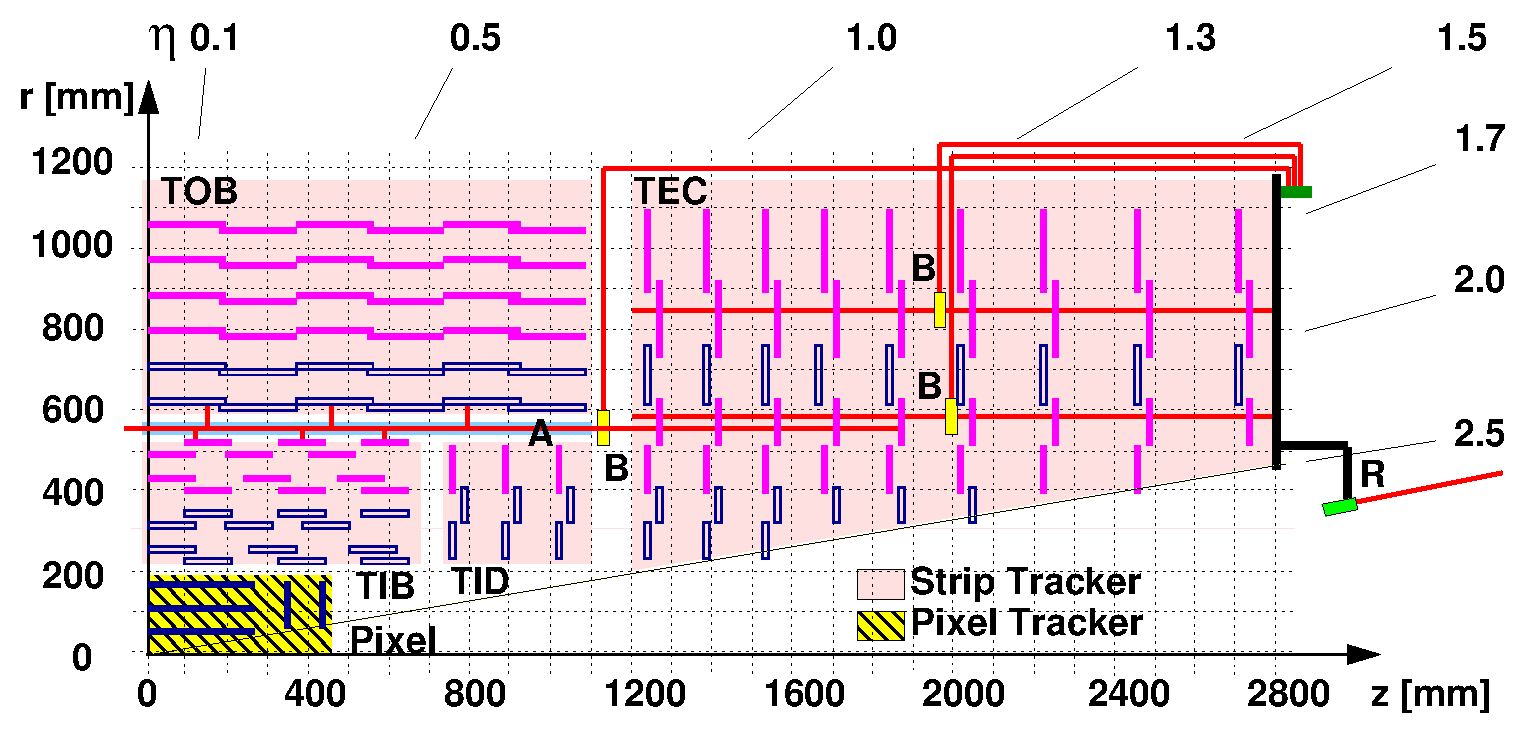
\includegraphics[width=.8\linewidth]{Experiment/figures/TrackerSystemLAS.eps}
\caption[Geometry of the Tracker System]{Tracker cross-section (1/4 of the $z$ view). The pixel tracker is located at the innermost radii of the detector and is labeled in striped yellow. The strip tracker is composed of four regions: Tracker Inner Barrel (TIB), Tracker Outer Barrel (TOB), Tracker End Cap (TEC), and Tracker Inner Disks (TID). The blue pieces are double-sided modules while magenta are single-sided. In addition to the silicon sensors, an infrared laser alignment system is used to provide coarse calibration for the tracker.}
\label{fig:TrackerSystem}
\end{center}
\end{figure}

\begin{figure}[htbp]
\begin{center}
\includegraphics[width=.45\linewidth]{Experiment/figures/MuonTrackEfficiency.pdf}
\includegraphics[width=.45\linewidth]{Experiment/figures/PionTrackEfficiency.pdf}
\caption[Global Track Reconstruction Efficiency at CMS]{Global track reconstruction efficiency of muons (left) and pions (right) for transverse momenta of 1, 10, and 100 $\rm{GeV}/c$. Overall efficiency decreases for smaller $p_T$ and near the edges of the detectable region.}
\label{fig:TrackEfficiency}
\end{center}
\end{figure}

As the tracker subsystem is the only one that can reconstruct vertices, great care is taken to affirm that the numerous pieces of the tracker are aligned to very high precision (ideally smaller than the hit resolution, so $\lesssim10\mu\rm{m}$). After construction, a laser alignment system is used to calibrate the tracker, as well as other subsystems, to account for shifts in orientation. However, this method primarily accounts for large scale misalignments and not individual modules. In sum, there are 9.6 million strips and 66 million silicon pixels spread across over 16000 modules, where the position and orientation of each must be tracked independently both before and during operation of CMS. The only way to get the desired detector position resolution is to use track-based alignment.

After measuring the positions of the various devices during construction and utilizing the laser alignment system, trajectories can be used to further the alignment. Since trajectories should be continuous, small misalignments of the modules will appear as discontinuities in the tracks and measuring their pull. In 2008, when the detector was fully constructed but the beam was not yet running, millions of cosmic muons were tracked through the detector. Computationally, to find the individual corrections, it is equivalent to minimizing a matrix equation for $O(10^5)$ degrees of freedom. Nevertheless, using a combined method of algorithms to find global and local correlations, the positions of the modules were determined to an average precision of 3-4 $\mu$m in the barrel and 3-14 $\mu$m in the endcap in the most sensitive coordinate~\cite{}. Since environmental conditions of operation can cause deviations, similar alignment strategies are used by CMS during data collection.

\subsection{Particle Identification}
\label{sec:ParticleID}

During operation, when the beams collide, all of the subsystems work in tandem to identify different particles by what portions they interact with. Muons and electrons will both record hits in the tracker, but the muon will move through the muon system while electrons stop in the ECAL. Fig.~\ref{fig:CMSSliceWithTracks} shows a diagram with the expected interactions from a sample set of particles. In theory, it seems like this should be simple categorization: only electrons and photons should interact with the ECAL, hadrons will interact with the HCAL, etc. Although it can be this simple, in practice, it is more nuanced. There are roughly 20-30 collisions per crossing and each can have multiple decay products which could deposit energies at similar locations; if a photon strikes the ECAL near an electron, how does CMS disentangle the two? Moreover, the lines between subdetectors aren't quite as strict. For example, neutral pions will commonly decay to two photons and thus could mimic a photon in the ECAL. Alternatively, decay in the ECAL can leak into the HCAL. CMS accounts for these \textit{fake rates} and makes proper identifications by using the \textit{particle-flow algorithm}~\cite{}. 

\begin{figure}[htbp]
\begin{center}
\includegraphics[width=.9\linewidth]{Experiment/figures/CMSSliceWithTracks.png}
\caption[Trajectories and Decays for Particle Identification in CMS]{Transverse slice of CMS with sample trajectories and decays from expected SM particles. Photons (dashed blue) and electrons will deposit their energy in the Electromagnetic Calorimeter, while both neutral (dashed green) and charged hadrons (green) deposit in the Hadronic Calorimeter. Muons (blue) will move through the muon system. All charged particles will interact with the tracker, leaving curved trajectories.}
\label{fig:CMSSliceWithTracks}
\end{center}
\end{figure}

Particle-flow links the output from the different subdetectors to iteratively identify particles. For charged particles, there will be tracks that would align with energy deposits in the calorimeters or the muon system. The hits in the calorimeters are clustered by looking for local maxima and associating nearby elements that are above threshold. In some cases, additional information can be used with the clustering. For example, in the ECAL, electrons will spread energy over a larger area that converted photons. These clusters (or trajectories in the muon system) are then matched to trajectories in the tracker system. Starting with a very tight cut between the two elements, matched particles and their associated hits in the subdetectors are removed from consideration and the algorithm repeats with a looser constraint.

This algorithm removes elements in a particular order\footnote{This is roughly in order of resolution for the expected particle, where each identification has little influence on successive identifications.}, starting with global muons, then electrons and photons, and finishing with jets. Once all particles are reconstructed, the missing transverse energy can be calculated. Finally, isolation can be used to indicate whether a given reconstructed particle is a \textit{prompt}, meaning that it comes from initial interaction. These reconstructed particles form the basic framework of all analyses at CMS. 

\subsection{Triggers}
\label{sec:Triggers}

As specified in Sec.~\ref{sec:LHC}, the intended number of collisions is on the order of 1 billion per second. However, only about 100 events per second can be stored for analysis, so nearly all of the events need to be rejected. Instead of arbitrarily taking data every hundredth of a second, a trigger system is designed so that only potentially interesting events can be captured. To determine what is interesting, data is temporarily stored and filtered by custom electronics. For the first trigger, Level-1, events are only accepted if they either have i) primitive objects from subdetectors that pass $p_T$ or $E_T$ thresholds or ii) global $E_T$ or missing transverse energy ($E_T^{miss}$ or MET). The detector elements with fast time resolution, like the RPCs in the muon system (see Sec.~\ref{sec:MuonSystem}), define these primitive objects. Altogether, the Level-1 trigger procedure, including data transfer and decision making, is designed to be completed within 3.2 $\mu\rm{s}$ and reduces the rate of events to approximately 100 kHz.

After passing the Level-1 trigger, high level triggers (HLTs) apply additional processing are used to further reduce the throughput. Where the Level-1 triggers use primitive objects, HLT cuts on approximately reconstructed objects, applying thresholds for observables like $p_T$, relative isolation in the calorimeters and/or tracker, or $|\eta|$ of the particle. Although a primary purpose of the HLT cuts is to bring the event rate to 100 Hz, these cuts are tuned to be broadly applicable to different analyses, being maximally inclusive to the intended signal while minimizing backgrounds. Each analysis group can then choose from the data that pass the appropriate high level triggers to make a high precision measurement, exclude a theoretical model, or discover a new as-yet undetected particle.

\section{Summary}
\label{sec:expt_summary}

In 2008, after 25 years of construction, the LHC began operation. Within another two years, the combined energy of the beams reached 7 $\rm{TeV}$. In 2011, over 5 $\mathrm{fb}^{-1}$ was collected for 7 $\rm{TeV}$. After increasing the energy to 8 $\rm{TeV}$ in 2012, nearly another 20 $\mathrm{fb}^{-1}$ was collected. This was sufficient to confirm the existence of a Higgs-like boson, appearing to achieve one of the most elusive discoveries in particle physics. This chapter has reviewed the intricacies of the detector itself, explaining the mechanism used to extract relevant information from the decays of trillions of high energy proton collisions. But how exactly was the new particle found in this mountain of data and can we measure its properties? Put bluntly, is this really the Higgs we've been looking for?
\chapter{Higgs Phenomenology at the LHC}
\label{sec:pheno}
\chaptermark{Higgs Phenomenology at the LHC}

\section{Summary}
\label{sec:pheno_summary}
\chapter{Higgs Discovery in $ZZ\rightarrow4l$}
\label{sec:discovery}
\chaptermark{Discovery}

\begin{center}
\begin{footnotesize}
\textit{\textbf{Vladimir}: That passed the time.\\
\textbf{Estragon}: It would have passed in any case.\\
\textbf{Vladimir}: Yes, but not so rapidly.}\\
Samuel Beckett, ``Waiting for Godot"
\end{footnotesize}
\end{center}

\section{Object Definitions}
\label{sec:zz4lObjects}

As specified in Sec.~\ref{sec:HiggsDecay}, $H\rightarrow ZZ \rightarrow 4l$ should be ideal for Higgs discovery. In this channel, we need four good lepton tracks for kinematic decay reconstruction, any relevant radiated photons for proper energy measurements, and a collection of any jets to examine the production of any resonance. Although rough reconstructions were defined in Sec.~\ref{sec:ParticleID}, our objects must be explicitly defined to examine the certainty of any results. To do so, we need four\footnote{Although the tau is also a lepton, it decays quickly and tends to appear more like a jet making the mass resolution of a $H\rightarrow ZZ \rightarrow 2l2\tau$ worse than a $4l$ event. For this reason, taus are not considered in the $H\rightarrow ZZ \rightarrow 4l$ analyses in this thesis.} objects: electrons, muons, photons, and jets.

\subsection{Electrons}
\label{sec:zz4lElectrons}

Electrons are geometrically constrained such that $|\eta^e|<2.5$, with a $p_T^e>7$ $\rm{GeV}$ cut is applied to maintain reasonable reconstruction efficiency while preserving capability to find low mass Higgs candidates. As referenced in Sec.~\ref{sec:ParticleID}, to reconstruct an electron, usually clusters of energy deposits in the ECAL are used as seeds to match to tracks from the silicon tracker (``outside-in" approach). However, to improve efficiency of low $p_T$ electrons, the opposite approach is also taken where trajectories are used to find clusters in the ECAL (``inside-out"). As electrons pass through the tracker volume, there will be some energy loss via bremsstrahlung which is modeled and fit using a gaussian sum filter. More details on the reconstruction algorithm is found in \cite{,,}. The expected energy resolution for prompt and isolated (see Sec.~\ref{sec:zz4lIsolation}) electrons is found in Fig.~\ref{fig:ElectronEnergyResolution}.

\begin{figure}[htbp]
\begin{center}
\includegraphics[width=.6\linewidth]{HiggsDiscovery/figures/effRMSbarrel_withregression_new.pdf}
\caption[Expected Energy Resolution for Electrons]{Expected energy resolution for prompt and isolated electrons in the ECAL barrel as a function of the initial energy. The effective resolution is better in the tracker (open blue squares) for low energy electrons, while the ECAL has better resolution for high energy electrons (open red circles). This encourages the use of both outside-in and inside-out techniques. The effective resolution (solid black circles) is $\lesssim 4\%$ of the initial energy. }
\label{fig:ElectronEnergyResolution}
\end{center}
\end{figure}

For identification, a Boosted Decision Tree\footnote{BDTs are a subset of the broader machine learning technique, decision tree learning, which utilizes multiple decision trees to classify data.} (BDT) multivariate technique \cite{} is trained using observables for electrons, such as the amount of energy radiated via bremsstrahlung during flight, matching between trajectories and ECAL clusters, and shower shapes in the ECAL. This method improves the resolution by $\sim 10\%$ per electron compared to cut-based techniques.

Lastly, to validate the momentum scale of the electrons in the $4l$ channel, invariant mass distributions of data from well-known SM particles that decay to $e^+e^-$ are compared to analytical distributions. In the left plot of Fig.~\ref{fig:ElectronMassResolutionAndBias}, electrons with $p_T\gtrsim35$ $\rm{GeV}$ show a bias in the reconstructed mass within $\sim0.3\%$ across three different decays\footnote{$J/\Psi$ is a meson made of $c\bar{c}$ with mass $m_{J/\Psi}=3.1$ $\rm{GeV}$ while $\Upsilon$ is a meson made of $b\bar{b}$ with mass $m_{\Upsilon}=9.6$ $\rm{GeV}$. Along with the $Z$, they have masses greater than $2m_e$ or $2m_\mu$, so they can be used as references to validate mass reconstruction.} ($Z$, $J/\Psi$, $\Upsilon$) for multiple pseudorapidity ranges. A small mass shift appears for lower $p_T$ electrons, accounted for as a systematic in the signal mass scale. The effective mass resolution in $Z\rightarrow e^+e^-$, found in  the right plot of Fig.~\ref{fig:ElectronMassResolutionAndBias}, is below $4\%$ for the full range of the ECAL.

\begin{figure}[htbp]
\begin{center}
\includegraphics[width=.45\linewidth]{HiggsDiscovery/figures/scale-ptdep-8TeV.pdf}
\includegraphics[width=.45\linewidth]{HiggsDiscovery/figures/electron_resolution.pdf}
\caption[Mass Resolution and Bias from Di-electron Decays]{Mass Bias and Resolution between Data and MC Simulation for di-electron decays at $8$ $\rm{TeV}$. For bias measurement (left), $Z\rightarrow e^+e^-$ (blue: solid circles in barrel, open diamonds in $0.8<|\eta|<1.5$, open squares in endcaps) shows little mass bias for higher $p_T$ electrons For lower $p_T$ electrons, $Z\rightarrow e^+e^-$, $J/\Psi\rightarrow e^+e^-$ (solid red circles), and $\Upsilon\rightarrow e^+e^-$ (solid green circles) show a small bias, accounted for as a systematic the signal mass scale. The instrumental mass resolution (right) using $Z\rightarrow e^+e^-$ is less than $4\%$ across the full ECAL range. Electrons are categorized by location and quality of reconstructed electron (B is ECAL Barrel, E for ECAL Endcap. G are the highest quality electron reconstructions, S is for lower quality reconstructions in multiple clusters or with a large amount of bremsstrahlung).}
\label{fig:ElectronMassResolutionAndBias}
\end{center}
\end{figure}

\subsection{Muons}
\label{sec:zz4lMuons}

Muons are reconstructed similar to electrons, except that the matching is done between the inner tracker and the muon system. As with electrons, matching can be ``outside-in" starting with hits in the muon system or ``inside-out" starting with hits in the tracker. By geometric and efficiency constraints, reconstructed muons must have $|\eta^\mu|<2.4$ and $p_T^\mu>5$ $\rm{GeV}$ \cite{}. As muons primarily interact with the tracker and muon system, muons are identified using minimal requirements in the tracker systems to account for consistent trajectories while maintaining small energy deposits in the ECAL \cite{}. The momentum resolution for muons is $1.3-2.0\%$ in the barrel and up to $6\%$ in the endcaps.

Similar to electrons, the muon mass scale and resolution is found using $Z\rightarrow \mu^+\mu^-$, $J/\Psi \rightarrow \mu^+\mu^-$, and $\Upsilon \rightarrow \mu^+\mu^-$ data and MC mass distributions. Across all decays, no bias is seen between data and MC within $0.1\%$, see left plot in Fig.~\ref{fig:MuonMassResolutionandBias}. Muons in the endcaps for the $J/\Psi$ decay have slightly larger offsets, but this is a very unlikely kinematic region for $H\rightarrow ZZ \rightarrow 4l$ events. In the right plot of Fig.~\ref{fig:MuonMassResolutionandBias}, mass resolution is seen to be consistent between data and MC within about $5\%$ for the $Z$ di-muon decay.

\begin{figure}[htbp]
\begin{center}
\includegraphics[width=.45\linewidth]{HiggsDiscovery/figures/100_scale_mf.pdf}
\includegraphics[width=.45\linewidth]{HiggsDiscovery/figures/100_resolution_mf.pdf}
\caption[Mass Resolution and Bias from Di-muon Decays]{Mass Bias (left) and Resolution (right) between Data and MC Simulation for di-muon decays: $Z\rightarrow \mu^+\mu^-$ (blue solid circles), $J/\Psi\rightarrow e^+e^-$ (red: solid circles in barrel, open diamonds in $0.8<|\eta|<1.2$, open squares in endcaps), and $\Upsilon\rightarrow e^+e^-$ (green: solid circles in barrel, open squares in endcaps). Aside from high $p_T$ muonic decays through endcaps, no bias is observed within about $0.1\%$. Mass resolution between $Z$ decays are in agreement within $5\%$.}
\label{fig:MuonMassResolutionandBias}
\end{center}
\end{figure}

\subsection{Lepton Isolation and Photons}
\label{sec:zz4lIsolation}

After reconstruction and identification, leptons should be isolated to confirm that they are a primary decay product. For any given particle flow candidate, the idea of relative isolation is defined by looking at all particles in a cone around the candidate and finding the relative fraction of $p_T$ from particles coming from non-leptonic processes. This is simply affirming that the lepton is the highest momentum object within a given space of the detector. Explicitly, for a cone of size $\Delta R = \sqrt{(\eta^l-\eta^i)^2 + (\phi^l-\phi^i)^2} < 0.4$, where $\eta^l,\phi^l$ are the $\eta$ and $\phi$ of the lepton candidate, the isolation $R_{iso}^l$ is
\begin{equation}
\label{eqn:reliso}
R_{iso}^l \equiv \left( \sum p_T^{\rm{charged}} + \rm{MAX}\left[0, \sum p_T^{neutral} + \sum p_T^{\gamma} - \rho\times A_{\rm{eff}}\right] \right) / p_T^{l}.
\end{equation}

$\sum p_T^{\rm{charged}}$ is the sum of the transverse momentum of any charged hadrons coming from the primary vertex, where the primary vertex is the vertex with the highest $\sum p_T^2$ of constituent tracks. $\sum p_T^{neutral}$ and $\sum p_T^{\gamma}$ are the sums of neutral hadrons and photons that are not radiated by the lepton (see below). When considering particles in this cone, particles very close to the lepton are not considered to avoid double counting.

As stated in Sec.~\ref{sec:ParticleID}, in any event, there are roughly 20-30 different collisions. After identifying the lepton candidates, the subsystems will still have some occupancy from the remaining collisions, called \textit{pileup}. The maximum and the $\rho\times A_{\rm{eff}}$ term in Eqn.~\ref{eqn:reliso} come from mitigating these effects in the neutral components, as the elements of the subsystems will have an average energy density from unassociated processes \cite{}. All isolated leptons in this analysis must have $R_{iso}^l < 0.4$.

After reconstruction, identification, and isolation, the overall efficiencies of electrons and muons are measured using a ``tag and probe" technique \cite{}. Using the large $Z\rightarrow l^+l^-$ dataset, one lepton (either an electron or a muon, depending on what efficiency is being evaluated) that passes all trigger, identification, and selection requirements is used as the ``tag". The $Z\rightarrow l^+l^-$ with background mass shape is then fit using samples where the second lepton, the ``probe", passes or fails the selection cuts. By finding the ratio of efficiencies between data and MC distributions with all associated uncertainties, the simulations can be reweighted in bins of $p_T^{l}$ and $\eta^l$ to account for the overall efficiency. Seen in Fig.~\ref{fig:LeptonEfficiencies}, both electrons and muons have high efficiencies for high $p_T$ leptons ($\gtrsim85\%$ and $\gtrsim97\%$, respectively).

\begin{figure}[htbp]
\begin{center}
\includegraphics[width=.45\linewidth]{HiggsDiscovery/figures/electron_efficiency.pdf}
\includegraphics[width=.45\linewidth]{HiggsDiscovery/figures/muon_efficiency.pdf}
\caption[Overall Efficiencies of Electron and Muon Reconstruction and Selection in $4l$ Analysis]{Efficiencies of reconstruction and selection for electrons (left: circles in barrel, squares in endcaps) and muons (right: circles in barrel, squares in endcaps) as functions of $p_T$, found using the tag and probe technique on simulation and data of $Z\rightarrow l^+l^-$. }
\label{fig:LeptonEfficiencies}
\end{center}
\end{figure}


Although photons are not part of this final decay channel, a lepton that decayed from the $Z$ could radiate a photon in its flight through the detector. To properly reconstruct the full kinematics, these \textit{final state radiation} (FSR) photons must be accounted for. FSR photons, having radiated from a lepton, must be close to a lepton candidate and have sufficient momentum to be considered a significant correction. Photons are accepted as FSR if: i) they fall in similar geometric boundaries as leptons ($|\eta^\gamma|<2.4$) and ii) have $p_T>2$ $\rm{GeV}$ if within $\Delta R < 0.07$ of a lepton OR $p_T>4$ $\rm{GeV}$ if found isolated within $0.07 < \Delta R < 0.5$ of a lepton candidate. An isolated photon is defined, similar to Eqn.~\ref{eqn:reliso}, as $R_{iso}^{\gamma} = (\sum p_T^{charged} + \sum p_T^{neutral} + \sum p_T^{photons})/p_T^\gamma < 1$ where the sums the same except over a cone of $\Delta R < 0.3$.

\subsection{Jets}
\label{sec:zz4lJets}

Once any lepton and FSR photon candidates are determined, jet candidates are identified. Jets are found using the HCAL and tracker, where they are reconstructed using the anti-$k_T$ clustering algorithm\footnote{As stated in Sec.~\ref{sec:HadrCalo}, jets come from the hadronization and fragmentation of particles that interact via the strong force. Different clustering algorithms have been developed to group tracks and calorimeter hits inside cones into jet objects.} \cite{} with distance parameter $R=0.5$, implemented using the {\tt FASTJET} package \cite{}. Jet energy corrections as functions of $E_T$ and $\eta$ are applied to calibrate the energy of a detected jet with the expected true energy \cite{}. To separate jet candidates from pileup, a discriminant is built \cite{} via a multivariate analysis using BDTs where the number vertices, jet shapes, relative multiplicity of charged and neutral components, and fraction of low-$p_T$ components are used for training. The tracks of any selected jets must be compatible with the primary vertex, as true for lepton candidates. Finally, jets must also have sufficiently high momentum ($p_T>30$ $\rm{GeV}$) and separated from any leptons or FSR photons ($\Delta R = \sqrt{(\eta^{l/\gamma}-\eta^{jet})^2 + (\phi^{l/\gamma}-\phi^{jet})^2} > 0.5$).

\section{MC and Datasets}
\label{sec:ZZ4lMCandData}

With objects defined, MC samples are generated for both background and signal processes. These samples can establish optimal event selections and quantify uncertainties. The full list of MC Samples can be found in Table~\ref{tbl:MCSamples}. 

\begin{table}[htbp]
  \begin{center}
  \vspace*{0.3cm}
  \renewcommand{\arraystretch}{0.5}
    \begin{tabular}{lllll} 
\hline %---------------------------------------------------------------------------------------------------------------------------------------------------------------------------- 
\small      \bf{Process} 		& \small \bf{MC}			& \multicolumn{2}{c}{\small\boldmath{$\sigma_{(N)NLO} $}} & \small\bf{ Comments and sample name}  \\
     					& \small \bf{generator}			& \small $7$ $\rm{TeV}$ 	& \small $8$ $\rm{TeV}$        			  &		                          \\ 
\hline \hline %=====================================================================================================================================================================
%
         \multicolumn{5}{l}{\small  \bf{Higgs boson}   $H \rightarrow ZZ \rightarrow 4\ell$} \\
%     	      
\small         ${gg} \rightarrow H$ & \small{\tt POWHEG}  & \small [1-20] fb 	& \small [1.2-25] fb        & \small{\small $\mathrm{m_{H}=110}$-$1000$ $\rm{GeV}$}  \\ 
\small         $VV \rightarrow H$   & \small{\tt POWHEG}  & \small [0.2-2] fb 	& \small [0.3-25] fb        & \small{\small $\mathrm{m_{H}=110}$-$1000$ $\rm{GeV}$}  \\ 
\small         $V^{*} \rightarrow VH$   & \small{\tt PYTHIA}  & \small [] fb 	& \small [] fb        & \small{\small $\mathrm{m_{H}=110}$-$200$ $\rm{GeV}$}  \\ 
\small         $t\bar{t}H$   & \small{\tt PYTHIA}  & \small [] fb 	& \small [] fb        & \small{\small $\mathrm{m_{H}=110}$-$200$ $\rm{GeV}$}  \\ 
\hline %---------------------------------------------------------------------------------------------------------------------------------------------------------------------------- 
         \multicolumn{5}{l}{{\small   \bf ZZ continuum } } \\
\small    $ q\bar{q} \rightarrow ZZ \rightarrow 4e(4\mu,4\tau) $           
                                    	  & \small{\tt POWHEG}	& \small 66.09 fb	& \small 76.91 fb	    & \small{\small ZZTo4e(4mu,4tau)}  \\ 
\small	 $ q\bar{q} \rightarrow ZZ \rightarrow 2e2\mu  $           
                                    	  & \small{\tt POWHEG}	& \small 152 fb	& \small 176.7 fb	    & \small{\small ZZTo2e2mu}  \\ 
\small	 $ q\bar{q} \rightarrow ZZ \rightarrow 2e(2\mu)2\tau  $           
                                    	  & \small{\tt POWHEG}	& \small 152 fb	& \small 176.7 fb	    & \small{\small ZZTo2e(2mu)2tau}  \\ 
\small      ${gg} \rightarrow ZZ \rightarrow 2\ell 2\ell'$              
      					  & \small{\tt gg2ZZ}  	& \small 3.48 fb 	& \small 12.03  fb	    & \small{\small GluGluToZZTo2L2L} \\ 
\small      ${gg} \rightarrow ZZ \rightarrow 4\ell$                
         				  & \small{\tt gg2ZZ}  	& \small 1.74 fb 	& \small 4.8 fb	    & \small{\small GluGluToZZTo4L} \\  
					 \hline
         \multicolumn{5}{l}{{\small  \bf Other di-bosons} } \\
\small	 $WW\rightarrow 2\ell2\nu $   & \small{\tt Madgraph}  & \small 4.88 pb   	& \small 5.995 pb 	    & \small{\small WWJetsTo2L2Nu} \\ 
\small	 $WZ\rightarrow 3\ell\nu $    & \small{\tt Madgraph}  & \small 0.868 pb 	& \small 1.057 pb  	    & \small{\small WZJetsTo3LNu} \\  
\hline %---------------------------------------------------------------------------------------------------------------------------------------------------------------------------- 
         \multicolumn{5}{l}{\small   \boldmath{$t\bar{t}$ and single $t$ }} \\
\small   $t\bar{t} \rightarrow \ell^+\ell^- \nu\bar{\nu} b\bar{b}$ & \small{\tt POWHEG}		& \small 17.32 pb    & \small 23.64 pb 	& \small{\small TTTo2L2Nu2B} \\       
\small   $t$ ($s$-channel)   		& \small{\tt POWHEG} 		& \small 3.19 pb 	& \small 3.89 pb 			& \small{\small T\_TuneXX\_s-channel} \\        
\small   $\bar{t}$ ($s$-channel)   	& \small{\tt POWHEG} 		& \small 1.44 pb 	& \small 1.76 pb 			& \small{\small Tbar\_TuneXX\_s-channel} \\       
\small   $t$ ($t$-channel)   		& \small{\tt POWHEG} 		& \small 41.92 pb 	& \small 55.53 pb				& \small{\small T\_TuneXX\_t-channel} \\        
\small   $\bar{t}$ ($t$-channel)   	& \small{\tt POWHEG} 		& \small 22.65 pb 	& \small 30.00 pb				& \small{\small Tbar\_TuneXX\_t-channel} \\
\small   $t$ ($tW$-channel)   		& \small{\tt POWHEG} 		& \small 7.87 pb 	& \small 11.77 pb				& \small{\small T\_TuneXX\_tW-channel-DR} \\        
\small   $\bar{t}$ ($tW$-channel)   	& \small{\tt POWHEG} 		& \small 7.87 pb 	& \small 11.77 pb				& \small{\small Tbar\_TuneXX\_tW-channel-DR} \\ 
\hline %---------------------------------------------------------------------------------------------------------------------------------------------------------------------------- 
          \multicolumn{5}{l}{\bf{Z/W + jets ($q=d,u,s,c,b$)}} \\     
\small   $W$ + jets     			& \small{\tt MadGraph}		& \small 31314 pb         & \small 36257.2 pb			& \small{\small WJetsToLNu} \\
\small   $Z$ + jets, m$_{\ell\ell}>50$     		& \small{\tt MadGraph}		& \small 3048 pb           & \small 3503.7 pb			& \small{\small DYJetsToLL*M-50} \\ 
\small   $Z$ + jets, $10<m_{\ell\ell}<50$     	& \small{\tt MadGraph}		& \small 12782.63 pb    & \small 915   pb			& \small{\small DYJetsToLL*M-10To50} \\ 
\hline %---------------------------------------------------------------------------------------------------------------------------------------------------------------------------- 
%          \multicolumn{5}{l}{ \small  \bf{QCD inclusive multi-jets}, {\small binned  $\Hat{p}_T^{\rm min}$}} \\    
%{\small $b,c \rightarrow e + X$}   	& \small{\tt PYTHIA}		& \small		& \small				& \small {\small QCD\_Pt-XXtoYY\_BCtoE }   \\
%\small  EM-enriched   			& \small{\tt PYTHIA}		& \small		& \small				&\small {\small QCD\_Pt-XXtoYY\_EMEnriched } \\
%\small   MU-enriched   			& \small{\tt PYTHIA}		& \small 		& \small				& \small {\small QCD\_Pt-XXtoYY\_MuPt5Enriched }  \\ 
%\hline%---------------------------------------------------------------------------------------------------------------------------------------------------------------------------- 
   \end{tabular}
\caption[MC Samples for $H\rightarrow ZZ\rightarrow 4l$]{Full List of MC Samples generated for $H\rightarrow ZZ\rightarrow 4l$, with their respective processes, generators, cross-sections for $\rm{7}$ $\&$ $\rm{8}$ $\rm{TeV}$ at the generated order, and sample names.}
  \label{tbl:MCSamples}
  \end{center}
\end{table}

For signal samples, gluon-gluon fusion and vector boson fusion are generated at next-to-leading order using {\tt POWHEG} \cite{} up to masses of $m_H = 1000$ $\rm{GeV}$. Higgs produced via Higgsstrahlung ($WH$ or $ZH$) or associated production ($t\bar{t}H$) are generated using {\tt PYTHIA} \cite{} at LO. Since their expected cross sections are smaller for higher masses (see Fig.~\ref{fig:HXSWGProduction}), they are only generated up to $m_H=200$ $\rm{GeV}$.

There are two additional complications for the Higgs signal samples. First, for lower masses, the Higgs can be modeled to have approximately zero-width, that is the mass distribution in $m_{4l}$ will be a very narrow resonance. For a higher mass Higgs, the number of energetically viable decay modes increases, so this approximation breaks down\footnote{This approximation also isn't entirely valid for a lower mass Higgs, as we shall see in Sec.~\ref{sec:Width}.} around $m_H \approx 400$ $\rm{GeV}$, as seen in Fig.~\ref{fig:HiggsWidth}. To account for this, the mass shape uses the complex-pole scheme \cite{,,}. Second, gluon-fusion Higgs production with $4l$ decay has identical initial and final states as the $gg\rightarrow 4l$ background, so they will interfere (see Sec.~\ref{sec:FeynDiagrams}, diagrams with identical initial and final states can interfere). Below $2\times m_Z$, this effect is negligible, because the $gg\rightarrow 4l$ background is small, but it must be accounted for in high mass Higgs samples. Additionally, signal events are reweighted to the total $pp\rightarrow H$ cross section, including NNLO and next-to-next-to-leading log\footnote{Corrections from additional Feynman diagrams can also have logarithmic dependencies.} corrections for gluon fusion \cite{} and NNLO contributions for VBF \cite{}.

\begin{figure}[htbp]
\begin{center}
\includegraphics[width=.5\linewidth]{HiggsDiscovery/figures/HiggsWidth}
\caption[Higgs Width as a Function of $m_H$]{Higgs Width as a Function of $m_H$. The width of the mass shape for the Higgs depends on the available decay modes at a given mass. For $m_H > 2\times m_Z$, both bosonic decays will be on-shell (see Sec~\ref{sec:HiggsDecay}), drastically increasing the width compared to low $m_H$.}
\label{fig:HiggsWidth}
\end{center}
\end{figure}

We can categorize background into \textit{reducible} and \textit{irreducible} backgrounds. Reducible backgrounds come from large cross section SM processes where two prompt isolated leptons are generated and the remaining two, coming from secondary decays unrelated to the desired $ZZ\rightarrow 4l$ vertex, are misidentified leptons. $Z$ + jets, for example, can have two isolated leptons from the $Z$ but occasionally two $b$-jets will be produced which can be misidentified as leptons. Similarly, $t\bar{t}$ commonly decays to a state with $l^+l^-b\bar{b}$. $W/Z$ + jets samples are produced using {\tt MADGRAPH} \cite{}, while any $t$ samples are made using {\tt POWHEG}. As the name implies, a smart selection (see Sec.~\ref{sec:ZZ4lSelection}) can reduce this background substantially.

Irreducible backgrounds are SM processes that have identical decay channels as the intended Higgs signal events, arising from the $ZZ$ continuum background. The primary irreducible background is $q\bar{q}\rightarrow 4l$, as seen in the left diagram of Fig.~\ref{fig:IrreducibleBackFeyn}, generated at NLO using {\tt POWHEG}. $gg \rightarrow 4l$, in the right diagram of Fig.~\ref{fig:IrreducibleBackFeyn}, is the subdominant irreducible background as it requires one loop to be produced. It was generated using {\tt GG2ZZ} \cite{}.

\begin{figure}
\begin{center}
\unitlength=1mm
\subfloat{
\begin{fmffile}{HiggsDiscovery/figures/qqZZBackground}
\begin{fmfgraph*}(60,40)
  \fmfstraight
  \fmfleft{i1,i2}
  \fmfright{sp1,sp2,sp3,sp4}
  \fmf{fermion,label=$q$,label.side=left,tension=2}{i1,v1}
  \fmf{fermion}{v1,v2}
  \fmf{fermion,label=$\bar{q}$,label.side=left,tension=2}{v2,i2}
  \fmf{photon,label=$Z/\gamma$}{v1,vo1}
  \fmf{photon,label=$Z/\gamma$}{v2,vo2}
  \fmf{phantom}{vo1,vo2}
  \fmf{phantom,tension=2}{vo1,sp1}
  \fmf{phantom,tension=2}{vo2,sp4}
  \fmffreeze
  \fmf{fermion,label=$l^{+}$,label.side=left}{sp1,vo1}
  \fmf{fermion,label=$l^{-}$}{vo1,sp2}
  \fmf{fermion,label=$l^{+}$,label.side=left}{sp3,vo2}
  \fmf{fermion,label=$l^{-}$}{vo2,sp4}
\end{fmfgraph*}
\end{fmffile}
}
\subfloat{
\begin{fmffile}{HiggsDiscovery/figures/ggZZBackground}
\begin{fmfgraph*}(60,40)
  \fmfstraight
  \fmfleft{i1,i2} \fmfright{o1,o2,o3,o4}
  \fmf{gluon,label=$g$,tension=2}{i1,v1} \fmf{gluon,label=$g$,tension=2}{i2,v2}
  \fmf{fermion}{v1,v2}
  \fmf{fermion}{v3,v4}
  \fmf{fermion,label=$q$,tension=2}{v2,v3}
  \fmf{fermion,label=$\bar{q}$,tension=2}{v4,v1} 
  \fmf{phantom,tension=2}{v4,o1}
  \fmf{phantom,tension=2}{v3,o4}
  \fmffreeze
  \fmf{photon,label=$Z/\gamma$,l.s=right}{v4,vo1}
  \fmf{photon,label=$Z/\gamma$}{v3,vo2}
  \fmf{fermion,label=$l^{+}$,label.side=left,l.d=2}{o1,vo1}
  \fmf{fermion,label=$l^{-}$,label.side=left,l.d=2}{vo1,o2}
  \fmf{fermion,label=$l^{+}$,l.s=left,l.d=2}{o3,vo2}
  \fmf{fermion,label=$l^{-}$,l.s=left,l.d=2}{vo2,o4}
\end{fmfgraph*}
\end{fmffile}
}
\end{center}
\caption[Irreducible $ZZ$ Backgrounds in the $4l$ Channel]{Feynman Diagrams for the Irreducible Backgrounds in the $4l$ channel. $q\bar{q}\rightarrow 4l$ (left) is dominant, while $gg\rightarrow 4l$ (right) requires a loop and is subdominant.}
\label{fig:IrreducibleBackFeyn}
\end{figure}

All generated background and signal samples interface with {\tt PYTHIA} to produce hadronization and low-$p_T$ radiation effects. After this stage, every sample was processed through software built on {\tt GEANT4} \cite{} which simulates further decays and geometric acceptances in CMS, then reconstructs objects using the same algorithms applied on data, accounting for any pileup effects. For any LO generators, the PDF used for generation is {\tt CTEQ6L} \cite{}. For NLO generators, {\tt CT10} \cite{} is used. 

The datasets used are from the 2011 $7$ $\rm{TeV}$ and 2012 $8$ $\rm{TeV}$ runs, with luminosities of $5.1 fb^{-1}$ and $19.7 fb^{-1}$, respectively. Triggers that require at least a pair of leptons are used. For any double lepton trigger (di-electron, di-muon, or muon and electron), at least one lepton must have $p_T>17$ $\rm{GeV}$ and the other must have $p_T>8$ $\rm{GeV}$. A triple electron trigger is also used where the \textit{leading} (highest $p_T$) electron must have $p_T>15$ $\rm{GeV}$, the \textit{subleading} (second highest $p_T$) electron must have $p_T>8$ $\rm{GeV}$, and the third electron must have $p_T>5$ $\rm{GeV}$.

\section{Event Selection}
\label{sec:ZZ4lSelection}

After finding four prompt isolated leptons, most of the reducible background is already suppressed, but because the cross sections of the reducible processes are so large they should be minimized. For the $ZZ \rightarrow 4l$ decay, the $Z$ decays are prompt so all four leptons should appear to come from one common vertex. Upon reconstruction of a primary vertex, the three dimensional distance of closest approach for a trajectory is called the \textit{impact parameter}, which has an associated uncertainty of $\sigma_{\rm{IP}}$. To confirm a common vertex, a cut of $|\rm{SIP_{3D}}=\frac{\rm{IP}}{\sigma_{\rm{IP}}}|<4$ is applied. Leptons that fail either the $|\rm{SIP_{3D}}|<4$ cut or the earlier $R_{iso}^l<0.4$ cut are considered \textit{loose} leptons\footnote{Loose leptons also have relaxed constraints on electron or muon identification but must be separated by at least $\Delta R>0.02$.}, to be used in the estimate of the reducible backgrounds (see Sec.~\ref{sec:ZZ4lMassShape}). On top of the $p_T$ cuts from any triggers, the leading lepton must have $p_T > 20$  $\rm{GeV}$ and the subleading lepton must have $p_T > 10$ $\rm{GeV}$ to improve efficiency.

Next, we construct $Z$ candidates out of the available leptons. The pair of opposite charge and matching flavor leptons (e.g. $e^+e^-$ and $\mu^+\mu^-$) with an invariant mass closest to $m_Z$ is considered $Z_1$, such that $40< m_{Z1} < 120$ $\rm{GeV}$. This cut eliminates nearly all backgrounds that do not contain a leptonic $Z$ decay (e.g. $t\bar{t}$, $W$ + jets) as it is unlikely to get an invariant mass near $m_Z$ otherwise.

Out of the remaining isolated leptons, another pair of opposite charge matching flavor leptons form $Z_2$. For a lower mass Higgs, it's expected that one $Z$ would be on-shell while the other would be off-shell. To optimize for these low mass signals\footnote{For Higgs events with $m_H > 2m_Z$, both of the $Z$ candidates should be on-shell which is accounted for by restricting $m_Z1,2 < 120$ $\rm{GeV}$.}, $m_{Z2}$ has a looser mass cut such that $12 < m_{Z2} < 120$ $\rm{GeV}$. If there are multiple $Z_2$ candidates, as can be the case for five or more isolated leptons, the $Z_2$ candidate with the highest scalar sum of $p_T$ is chosen as these leptons should have the highest reconstruction efficiency. For both $Z_1$ and $Z_2$, if there are any FSR leptons associated with one of the constituent leptons, only those that bring $m_{Z1,2}$ closer to $m_Z$ are kept so long as $m_{ll\gamma}<100$ $\rm{GeV}$.

The requirement for $Z_2$ eliminates most of the remaining reducible $Z+X$ background for the same reason that the $Z_1$ cut eliminates other leptonic background. However, to avoid possible contamination from low-mass hadronic decays faking leptons, any opposite charge pairing of the selected four must have a sufficient invariant mass such that $m_{ll'} > 4$ $\rm{GeV}$. 

Finally, given the earlier direct exclusions from LEP (see Sec.~\ref{sec:findinghiggs}), a cut of $m_{4l} >100$ $\rm{GeV}$ is applied. After object definitions and selection cuts, the final efficiencies of signal detection as a function of the Higgs mass are seen in Fig.~\ref{fig:HiggsEffic}. In general, the $4\mu$ mode has the highest efficiency due to the quality of reconstruction compared to electrons. The relative increase in efficiency past $m_H \approx 200$ $\rm{GeV}$ comes from both $Z$ candidates being on-shell. Polynomial parameterizations are built for the MC signal mass points such that a full range of masses can be examined, as used in Sec.~\ref{sec:ZZ4lAnalysis}.

\begin{figure}[htbp]
\begin{center}
\includegraphics[width=.6\linewidth]{HiggsDiscovery/figures/Efficiency_ggH_8TeV.pdf}
\caption[Signal Efficiency of Gluon Fusion as a Function of $m_H$]{Signal detection efficiencies of ggF as functions of $m_H$, fit with polynomial curves estimated from MC simulation. $4\mu$ (red triangles) has the highest relative efficiency as muon have better selection efficiency, while $4e$ (green circles) has the lowest from electrons having worse efficiency. $2e2\mu$ (blue squares) is between the two. Efficiencies are produced for all production methods with similar results.}
\label{fig:HiggsEffic}
\end{center}
\end{figure}

\section{Likelihood Analysis}
\label{sec:ZZ4lAnalysis}

All observed events are split into tweleve different sub-categories: two for beam energy ($7$ or $8$ $\rm{TeV}$), three for final states ($4e$, $4\mu$, or $2e2\mu$), and two for jet categorization ($\geq2$ jets or $<2$ jets). The likelihood analysis is built on a three-dimensional model of observables: $m_{4l}$, $\mathcal{D}_{\rm{bkg}}^{\rm{kin}}$ and $p_T$ or $D_{jet}$, where the final observable is determined by the jet category. Instead of applying a full three-dimensional fit, the model is broken into three pieces which account for correlations. A probability distribution is defined for $m_{4l}$, while two-dimensional templates are defined for $(m_{4l},\mathcal{D}_{\rm{bkg}}^{\rm{kin}})$ and $(m_{4l},p_T$ or $D_{jet})$ where the respective templates are normalized for each slice of $m_{4l}$. The three-dimensional likelihood is therefore the product of the likelihood of a given mass and the likelihoods of a particular value of $\mathcal{D}_{\rm{bkg}}^{\rm{kin}}$ and $p_T$ or $D_{jet}$ given that mass. Explicitly, for each event:
\begin{equation}
\label{eqn:likelihoodXS}
\mathcal{L}_{3D}(m_{4l},\mathcal{D}_{\rm{bkg}}^{\rm{kin}},D_{jet})=\mathcal{L}(m_{4l}) \times \mathcal{L}(\mathcal{D}_{\rm{bkg}}^{\rm{kin}}|m_{4l}) \times \mathcal{L}(D_{jet}|m_{4l})
\end{equation}
where the first term defines the likelihood of the event having that $m_{4l}$, the second term defines the 2D template for the kinematic discriminant given $m_{4l}$, and the third term defines the 2D template for the production discriminant, either $p_T$ or $D_{jet}$, given $m_{4l}$. Each likelihood is detailed more explicitly in the following sections, where shape systematics are discussed for each component and common normalization systematics are detailed in Sec.~\ref{sec:ZZ4lSystematics}.

\subsection{Expected $m_{4l}$ Distributions}
\label{sec:ZZ4lMassShape}

To first order, any Higgs-like resonance should appear as an excess of events compared to what is expected from the SM background processes. To test different Higgs masses, the backgrounds must be well-defined across a wide range of $m_{4l}$. For the dominant $ZZ$ continuum backgrounds, the MC distributions are used as a baseline for the $m_{4l}$ shape. The cross sections of the $ZZ$ backgrounds are calculated to NLO using {\tt MCFM} \cite{}. These distributions are then fit with an analytic function to allow for a smooth distribution over the full range, where their normalizations are allowed to vary within uncertainties. Shape uncertainties are comparatively negligible.

For the reducible background, hereafter called $Z+X$, because most of the events from MC are eliminated by demanding four prompt leptons with two $Z$ objects, a data driven mass shape is used to account for all contributions. When MC simulations are sparsely populated, one can use a data driven technique by looking in a region of phase space adjacent to the signal region, typically called a \textit{control region}, to extrapolate back to the signal region. In the case of this analysis, using a dataset with $Z_1 + l_{\rm{loose}}$, construct $Z_2$ using same flavor lepton pairs where $m_{Z2} > 12$ $\rm{GeV}$ and $m_{4l} > 100$ $\rm{GeV}$. Two parallel methods are taken to estimate the reducible contribution with this sample, either the lepton pair that makes up $Z_2$ will have the same sign (SS) while passing all cuts or they are opposite sign (OS) but fail the selection cuts while passing the loose cuts. 

In the OS analysis, the mass of $Z_2$ is further constrained such that $|m_{Z2}-m_Z|<10$ $\rm{GeV}$. The dataset is then further split into two categories: after the two prompt leptons from $Z_1$ there are either no leptons passing the selection cuts (2P2F) or one lepton passing the selection cuts (3P1F). Unsurprisingly, the two categories largely correspond to the types of reducible background. $Z$ + jets and $t\bar{t}$ will tend to have two prompt leptons, while $WZ$ + jets will tend to have three with any other selection leptons coming from misidentified jets. To estimate the contribution from each category to the signal region, each event is reweighted by a factor that accounts for the misidentification of one or two nonsingular leptons. In the SS analysis, $Z_2$ is not as constrained with $|m_{Z2}-m_Z|<40$ $\rm{GeV}$. The extrapolation back to the signal region is then similar to 2P2F in the OS method, with an additional factor to account for the ratio of OS to SS control regions.

Both methods give similar expectations for the number of reducible background events in the signal region, with any uncertainties accounted for the final results. For the mass shape, the 2P2F and 3P1F events from the OS method are fit using analytical forms and combined to get the shape in Fig.~\ref{fig:ZXMassShapes}. This shape has an associated uncertainty coming from the choice of fit function and binning, seen as a yellow band.

\begin{figure}[htbp]
\begin{center}
\includegraphics[width=.6\linewidth]{HiggsDiscovery/figures/PredictedComponentsSR_withData_PAPER.pdf}
\caption[Reducible Background Mass Shapes]{$m_{4l}$ Distributions for Reducible Background. Contributions from $Z$ + jets, $Z+b\bar{b}$, and $t\bar{t}$ come from 2P2F category (solid green) of OS control region. $WZ$ and $Z\gamma$ + jets come from 3P1F category (dashed red). Each contribution is fit separately to form full prediction (blue curve with yellow band indicating total uncertainty) compared to data (black dots).}
\label{fig:ZXMassShapes}
\end{center}
\end{figure}

For signals, the nominal mass shapes for the expected masses are found via MC simulation. For each Higgs mass simulated, the mass distribution is fit with a relativistic Breit-Wigner distribution\footnote{The Breit-Wigner distribution is commonly used in particle physics, representing the probability of generating an unstable propagator, like the $Z$ or Higgs, at a given energy.} convoluted with a double-sided Crystal Ball function\footnote{The Crystal Ball is a function that is used to give a gaussian distribution a long-tail with power-law behavior. A double-sided Crystal Ball applies this long tail on both sides of the gaussian. In particle physics, this is useful to account for energy leakage in the tails of probability distributions.} \cite{}. For $m_H < 400$ $\rm{GeV}$, this function is fit for all production mechanisms, jet categories, decay modes, and beam energy, where the normalization will vary by the expected cross section for that production or categorization. These normalizations have associated systematics (see Sec.~\ref{sec:ZZ4lSystematics}), while any shape uncertainties are minimal since the experimental mass resolution of the detector being much larger than the expected widths. Sample distributions for the signal are found in Fig.~\ref{fig:LMHiggsShape}.

\begin{figure}[htbp]
\begin{center}
\includegraphics[width=.3\linewidth]{HiggsDiscovery/figures/fitM126_channel0.pdf}
\includegraphics[width=.3\linewidth]{HiggsDiscovery/figures/fitM126_channel1.pdf}
\includegraphics[width=.3\linewidth]{HiggsDiscovery/figures/fitM126_channel2.pdf}
\caption[Low Mass Higgs Signal Mass Shapes]{Sample Higgs signal $m_{4l}$ fits on MC simulation for $m_H=126$ $\rm{GeV}$ in ggF for $4\mu$ (left, red), $4e$ (middle, green), and $2e2\mu$ (right, blue) Each production method, beam energy, decay mode, and jet categorization has an independent fit for every mass point.}
\label{fig:LMHiggsShape}
\end{center}
\end{figure}

In the high mass region, $m_H \gtrsim 400$ $\rm{GeV}$, the mass shapes will change. As specified in Sec.~\ref{sec:ZZ4lMCandData}, the complex-pole scheme must be used and interference with the background is non-negligible, both of which enter into the signal $m_{4l}$ parameterizations via reweighting. After this reweighting, the Breit-Wigner constraint used for the lower masses is loosened by allowing the width to float such that it matches the MC distributions. Finally, instead of using the same mass shape for ggF and VBF, the shapes are found independently. The high mass $m_{4l}$ distributions have shape systematics arising from theoretical uncertainties in the applied corrections on top of any normalization systematics. Example high mass signal shapes with uncertainty bands are contained in Fig.~\ref{fig:HMHiggsShape}.

\begin{figure}[htbp]
\begin{center}
\includegraphics[width=.45\linewidth]{HiggsDiscovery/figures/H900_4mu_Reco_syst.pdf}
\includegraphics[width=.45\linewidth]{HiggsDiscovery/figures/VBFH900_4mu_Reco_syst.pdf}
\caption[High Mass Higgs Signal Mass Shapes]{Higgs signal $m_{4l}$ shapes for 900 $\rm{GeV}$ for ggF (left) and VBF (right). Dashed black line is shape directly from MC. Blue solid line accounts for complex-pole scheme reweighting and interference with backgrounds, where the red and green envelopes account for the uncertainty of reweighting.}
\label{fig:HMHiggsShape}
\end{center}
\end{figure}

These mass shapes can then be multiplied by the signal efficiencies, as discussed in Sec.~\ref{sec:ZZ4lSelection}, and the ratio for jet categorization, to be discussed in Sec.~\ref{sec:ZZ4lDjet}. This process gives the final yields for both the SM backgrounds and the Higgs signal as functions of $m_{4l}$ for any given Higgs mass to be evaluated.

\subsection{Kinematic Discriminant for Decay}
\label{sec:ZZ4lKD}

For any $4l$ event, the kinematic discriminant, $\mathcal{D}_{\rm{bkg}}^{\rm{kin}}$, can be constructed with the angular distributions of the decay. Eqn.~\ref{eq:MELADisc} defines the discriminant used, where the signal probability comes from the leading order {\tt JHUGen} matrix element and the background probability comes from the $q\bar{q}\rightarrow 4l$ LO matrix element found via {\tt MCFM}. Multiple sources for the matrix elements were tested with negligible differences. The relative normalization of the probabilities is tuned using a constant factor such that the total probability of signal plus background are equal above and below $\mathcal{D}_{\rm{bkg}}^{\rm{kin}} = 0.5$. No matrix element parameterization exists for $Z+X$, but the kinematic largely match those for $q\bar{q}\rightarrow 4l$ where a shape systematic is applied to account for any differences. Alternative methods using machine learning techniques, such as boosted decision trees or bayesian neural networks, show similar results to the matrix element approach. Two dimensional templates of $(m_{4l},\mathcal{D}_{\rm{bkg}}^{\rm{kin}})$ can be seen in Fig.~\ref{fig:MELATemplates}.

\begin{figure}[htbp]
\begin{center}
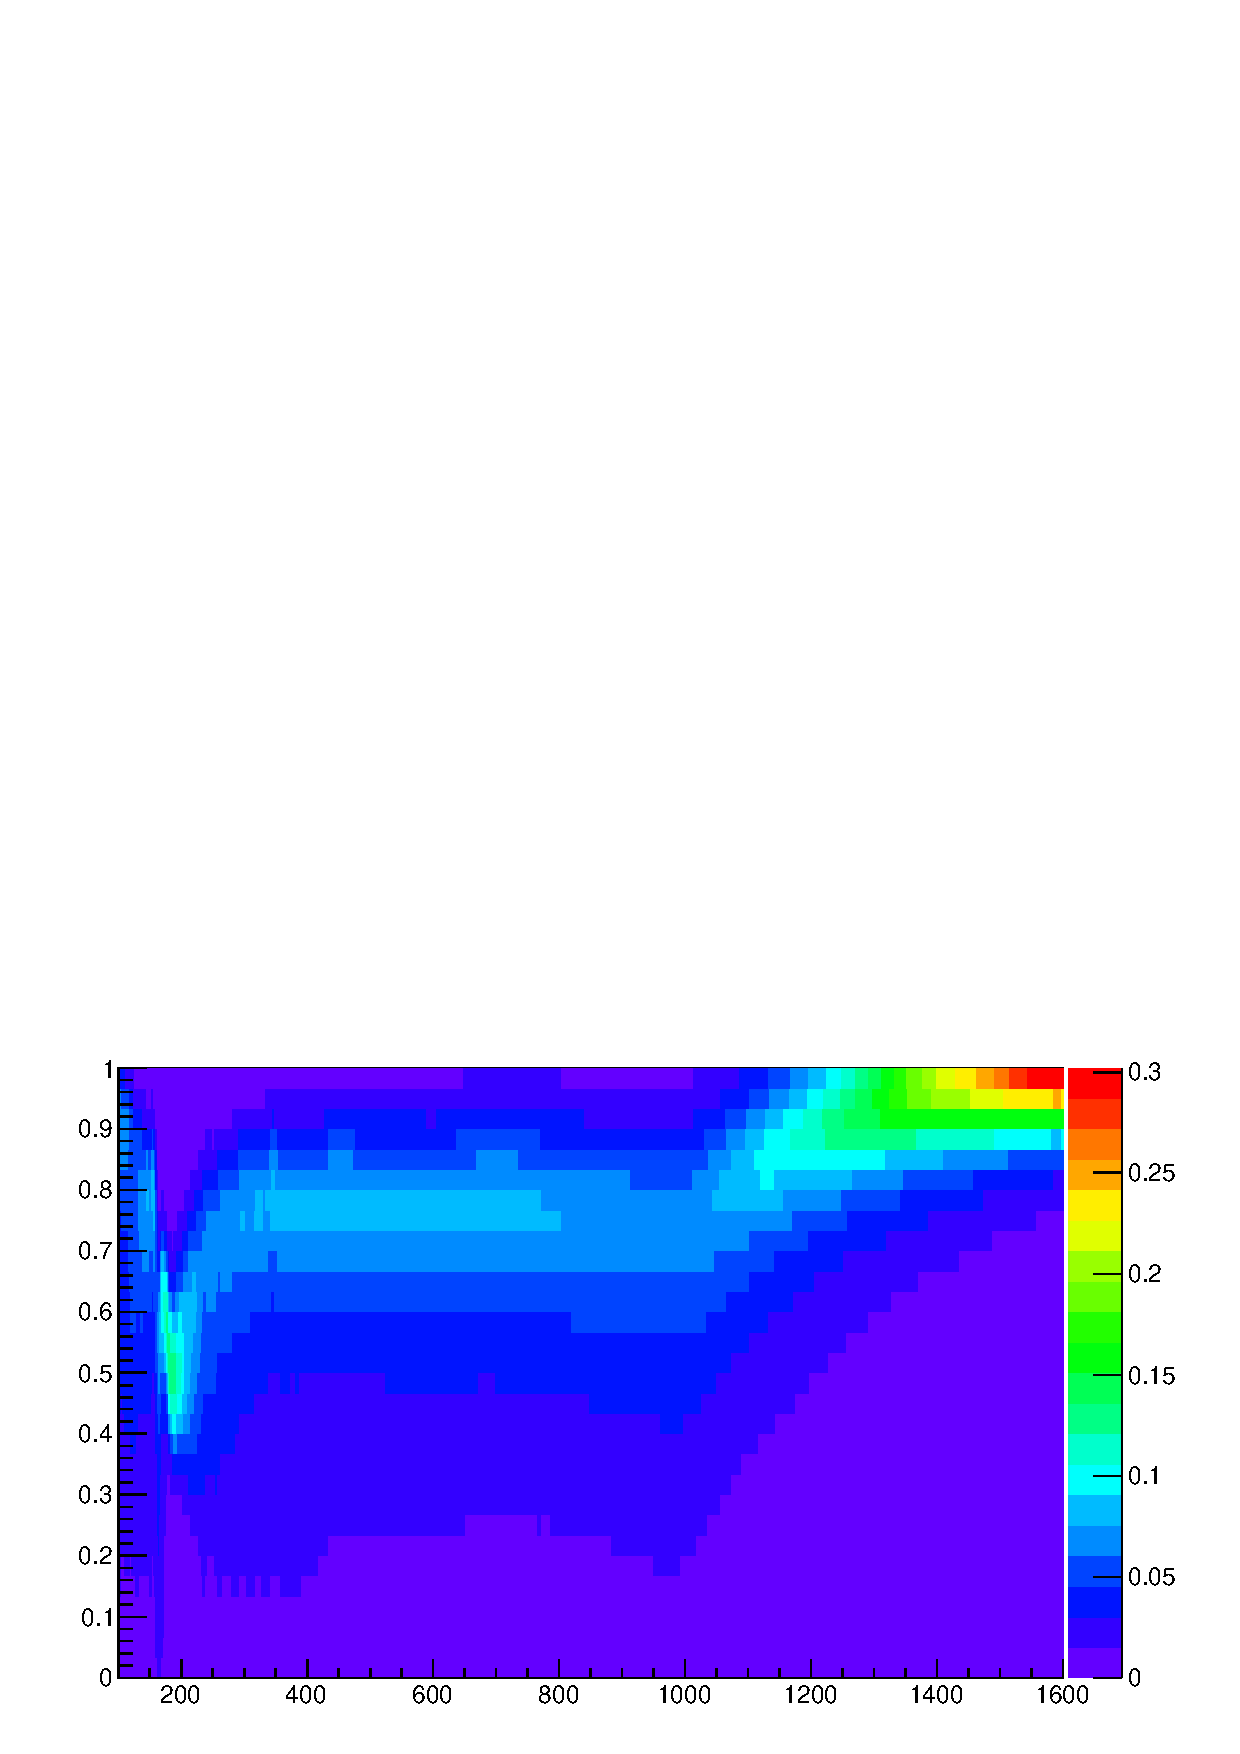
\includegraphics[width=.4\linewidth]{HiggsDiscovery/figures/Dsignal_2e2mu.pdf}
\includegraphics[width=.4\linewidth]{HiggsDiscovery/figures/Dbackground_qqZZ_2e2mu.pdf} \\
\includegraphics[width=.4\linewidth]{HiggsDiscovery/figures/Dbackground_ggZZ_2e2mu.pdf}
\includegraphics[width=.4\linewidth]{HiggsDiscovery/figures/Dbackground_ZX_2e2mu.pdf}
\caption[Templates of Kinematic Discriminant for $H \rightarrow ZZ \rightarrow 4l$]{Samples of $\mathcal{D}_{\rm{bkg}}^{\rm{kin}}$ v $m_{4l}$ templates for 8 $\rm{TeV}$ $2e2\mu$ Higgs signal(top left), $q\bar{q}\rightarrow ZZ$ (top right), $gg\rightarrow ZZ$ (bottom left), and $Z+X$ (bottom right) used in the analysis. Separate templates were made for $4e$, $4\mu$, and $2e2\mu$.}
\label{fig:MELATemplates}
\end{center}
\end{figure}

\subsection{Discriminating Production Mechanisms}
\label{sec:ZZ4lDjet}

As discussed in Sec.~\ref{sec:VBFVertex}, VBF events can be identified using the kinematics of the additional two jets over other production mechanisms or backgrounds. In that vein, after selection, events are categorized by their number of jets. The \textit{dijet} category encapsulates all events with at least two jets meeting the definitions in Sec.~\ref{sec:zz4lJets}. All other selected events fall into the \textit{non-dijet} category. On top of the signal selection efficiency, the dijet ratio is constructed as a function of $m_H$ (Figs.~\ref{fig:DijetRatioggHqqH} and~\ref{fig:DijetRatioAss}) to determine the expected number of expected signal and background events in a particular category and thus enters into the $m_{4l}$ distributions for each jet category.

\begin{figure}[htbp]
\begin{center}
\includegraphics[width=.3\linewidth]{HiggsDiscovery/figures/eff_ggH_4mu_ratio.pdf}
\includegraphics[width=.3\linewidth]{HiggsDiscovery/figures/eff_ggH_4e_ratio.pdf}
\includegraphics[width=.3\linewidth]{HiggsDiscovery/figures/eff_ggH_2e2mu_ratio.pdf} \\
\includegraphics[width=.3\linewidth]{HiggsDiscovery/figures/eff_qqH_4mu_ratio.pdf}
\includegraphics[width=.3\linewidth]{HiggsDiscovery/figures/eff_qqH_4e_ratio.pdf}
\includegraphics[width=.3\linewidth]{HiggsDiscovery/figures/eff_qqH_2e2mu_ratio.pdf}
\caption[Dijet Ratio of Gluon Fusion and Weak Vector Boson Fusion as Function of $m_H$]{Dijet ratio of ggF (top row) and VBF (bottom row) as functions of $m_H$. Left to right: $4\mu$, $4e$, $2e2\mu$. There should be very correlation between the Higgs final state and the dijet ratio, which is exactly what is seen.}
\label{fig:DijetRatioggHqqH}
\end{center}
\end{figure}

\begin{figure}[htbp]
\begin{center}
\includegraphics[width=.3\linewidth]{HiggsDiscovery/figures/eff_WH_2e2mu_ratio.pdf}
\includegraphics[width=.3\linewidth]{HiggsDiscovery/figures/eff_ZH_2e2mu_ratio.pdf}
\includegraphics[width=.3\linewidth]{HiggsDiscovery/figures/eff_ttH_2e2mu_ratio.pdf}
\caption[Dijet Ratio of Associated Production as Function of $m_H$]{Dijet ratio of WH (left), ZH (middle), and ttH (right). ttH inherently involves the production of two jets, so the ratio will be nearly 100\%.}
\label{fig:DijetRatioAss}
\end{center}
\end{figure}

Whether an event falls into the dijet or non-dijet category determines what observables are used for the analysis. In the non-dijet category, Higgs events, particularly those generated via other production mechanisms than ggF, will tend to have higher $p_T$ distributions, seen in Fig.~\ref{fig:HiggspT}. To aid in discrimination of production mechanisms, $p_T$ can be used as an observable in the non-dijet category.

For signal, $p_T$ distributions are found via analytic fits of MC simulation, with some reweighting for ggF high mass samples to account for theoretical limitations and to bring the LO $p_T$ distributions of associated Higgs production in agreement with NLO simulation. Shape systematics come from the choice of scales used theoretical predictions, top-mass approximation, and PDF uncertainties for ggF and VBF, while associated production methods have systematics from the reweighting procedure applied. For the irreducible $ZZ$ backgrounds, analytical fits come from MC reweighted to account for differences between data and MC \cite{}, where shape systematics are identical to VBF. $Z+X$, being data driven, is fit with a modified Tsallis function \cite{} where systematics come from uncertainty of the fit. Due to small differences in resolution based on $p_T$, there is a slight dependence of $\mathcal{D}_{\rm{bkg}}^{\rm{kin}}$ on $p_T$ which is accounted for in the shape systematics. Example 2D templates of $(p_T,m_{4l})$ to be used in the analysis are seen in Fig.~\ref{fig:pTTemplates}.

\begin{figure}[htbp]
\begin{center}
\includegraphics[width=.4\linewidth]{HiggsDiscovery/figures/pt_shape.pdf}
\caption[Transverse Momentum Shapes of Different Higgs Production Mechanisms]{$p_T$ distributions for ggF (hashed red), VBF (black), VH (blue), and the dominant $q\bar{q}$ background (hashed black). Subdominant production mechanisms have harder $p_T$ spectra than either ggF or the $q\bar{q}$ background, so it can used to discriminate production mechanisms.}
\label{fig:HiggspT}
\end{center}
\end{figure}

\begin{figure}[htbp]
\begin{center}
\includegraphics[width=.3\linewidth]{HiggsDiscovery/figures/ptrestricted_ggDefaultTemplate_8TeV.pdf}
\includegraphics[width=.3\linewidth]{HiggsDiscovery/figures/ptrestricted_vbfDefaultTemplate_8TeV.pdf}
\includegraphics[width=.3\linewidth]{HiggsDiscovery/figures/ptrestricted_zzDefaultTemplate_8TeV.pdf}
\caption[Templates of Transverse Momentum for $4l$ Signals and Background]{Samples of $p_T$ v $m_{4l}$ templates for 8 $\rm{TeV}$ ggF (left), VBF (middle), and $q\bar{q}\rightarrow ZZ$ (right) used in the analysis. Other templates were made and used for WH, ZH, and $gg\rightarrow ZZ$.}
\label{fig:pTTemplates}
\end{center}
\end{figure}

For any dijet event, the combined kinematics of the jets can be examined. In the initial discovery and property measurements of the Higgs, a matrix element technique was not yet developed so a linear discriminant \cite{} was built to optimize separation between VBF and ggF production mechanisms. Using the leading and subleading jets, $m_{JJ}$ and $\Delta\eta_{JJ}$ form the two variables for the discriminant. The optimal combination, trained on {\tt POWHEG} ggF and VBF samples, is
\begin{equation} \label{eq:HiggsFisher}
D_{jet} = 0.18\Delta\eta_{JJ} + 1.92\times10^{-4}m_{JJ}
\end{equation}
This formulation is then implemented for different MC samples (or control region for $Z+X$) to form the 2D $(m_{4l},D_{jet})$ templates. Shape systematics are applied for each template, coming from the largest deviations in available alternative shapes for the respective sample: choice of MC generator, choice of hadronization tuning, or jet energy scale corrections. Sample templates are seen in Fig.~\ref{fig:FisherTemplates}.

\begin{figure}[htbp]
\begin{center}
\includegraphics[width=.3\linewidth]{HiggsDiscovery/figures/deta_shape.pdf}
\includegraphics[width=.3\linewidth]{HiggsDiscovery/figures/mjj_shape.pdf}
\includegraphics[width=.3\linewidth]{HiggsDiscovery/figures/djet_shape.pdf} \\
\caption[Jet Kinematic Shapes of Different Higgs Production Mechanisms]{$\Delta\eta_{JJ}$ (left) and $m_{JJ}$ (middle) distributions for ggF (hashed red), VBF (black), VH (blue), and the dominant $q\bar{q}$ background (hashed black). These are used as input for the linear discriminant (right, defined in Eq.~\ref{eq:HiggsFisher}).}
\label{fig:HiggsFisher}
\end{center}
\end{figure}

\begin{figure}[htbp]
\begin{center}
\includegraphics[width=.3\linewidth]{HiggsDiscovery/figures/ggH_Fisher_2D.png}
\includegraphics[width=.3\linewidth]{HiggsDiscovery/figures/qqH_Fisher_2D.png}
\includegraphics[width=.3\linewidth]{HiggsDiscovery/figures/qqZZ_Fisher_2D.png} \\
\caption[Templates of $D_jet$ for Signals and Background]{Samples of $D_{jet}$ v $m_{4l}$ templates for ggF (left), VBF (middle), and $q\bar{q}\rightarrow ZZ$ (right) used in the analysis. Other templates were made and used for WH, ZH, $\rm{t\bar{t}H}$, $gg\rightarrow ZZ$, and $Z+X$. As there are no appreciable differences between decay mode (see Figs.~\ref{fig:DijetRatioggHqqH} and \ref{fig:DijetRatioAss}) nor beam energy, one 2D template is used for each production method or background.}
\label{fig:FisherTemplates}
\end{center}
\end{figure}

On top of any normalization or shape systematics applied, to account for the uncertainty of jet categorization, we used the suggestions of the JetMET group \cite{}. For ggF, a 15\% yield uncertainty is used for the non-dijet category and 30-50\% for the dijet category. Given that VBF inherently has two hard jets attached, the uncertainties used are lower: 10\% for the 0 jet category and 5\% for 1 or 2 jet categories.

\subsection{Systematics}
\label{sec:ZZ4lSystematics}

Broadly speaking, the systematics applied are split into two types: normalization uncertainties and shape uncertainties. Normalization uncertainties imply that there is an uncertainty on the overall number of events that will appear (e.g. for a particular decay mode, background). Shape uncertainties mean that there is uncertainty on how those events will appear, independent of the number (e.g. kinematics of the Higgs production, mass shape of the background). While shape systematics were discussed in earlier section with their respective shapes, Table~\ref{tbl:HZZ4lNormSyst} contains all common normalization systematics applied in this analysis for the $m_H = 126$ $\rm{GeV}$ mass point.

\begin{table}[htbp]
  \begin{center}
    \begin{tabular}{|lccccccc|}
      \hline
      Source         & \multicolumn{4}{c}{Signal ($m_H = 126$ $\rm{GeV}$)}  &  \multicolumn{3}{c|}{Backgrounds} \\
      \hline
      & ggF       & VBF     &  $VH$   &  $t\bar{t}H$ &  $q\bar{q}\rightarrow ZZ$  &  $gg\rightarrow ZZ$  & $Z+X$ \\
      \hline
      $\alpha_S$ + PDF ($gg$)           & 7.2\%         &  \NA      &   \NA                   &  7.8\%       &  \NA                     &  7.2\%            & \NA   \\
      $\alpha_S$ + PDF ($q\bar{q}$)    & \NA             &  2.7\%  &   3.5\%               &  \NA           &  3.4\%                 &  \NA                & \NA   \\
      Missing higher orders           & 7.5\%         &  0.2\%  &  0.4\%, 1.6\%         & 6.6\%        &  2.9\%                 &  24\%             & \NA   \\
      Signal acceptance               & \multicolumn{4}{c}{ 2\% }                                      &  \NA                     & \NA                 & \NA   \\
      BR($H\rightarrow ZZ$)              & \multicolumn{4}{c}{ 2\% }                                      &  \NA                     & \NA                 & \NA   \\
      Luminosity                      & \multicolumn{6}{c}{ 2.6\% }                                                                                 & \NA   \\
      Electron efficiency             & \multicolumn{6}{c}{ 10\% ($4e$),   4.3\% ($2e2\mu$)}                                                 & \NA   \\
      Muon efficiency                 & \multicolumn{6}{c}{ 4.3\% ($4\mu$), 2.1\% ($2e2\mu$)}                                                 & \NA   \\
      Control region                  & \NA             & \NA       & \NA                     & \NA            & \NA                      & \NA                 & 40\% \\
      \hline
    \end{tabular}
    \caption[Normalization Uncertainties in the $4l$ Discovery]{Normalization uncertainties for signal and background processes in $8$ $\rm{TeV}$ data for $m_H=126$ $\rm{GeV}$ in the non-dijet category. Values may change vary between mass points. $7$ $\rm{TeV}$ uncertainties are similar. Uncertainties on the same line are 100\% correlated except for missing higher orders which are uncorrelated and PDF ($gg$) for $t\bar{t}H$ which are anticorrelated.
      \label{tbl:HZZ4lNormSyst}}
  \end{center}
\end{table}

The parton distribution function (PDF), as discussed in Sec.~\ref{sec:HiggsProduction}, accounts for the production of different processes at hadronic colliders. Any uncertainty in the initial state can clearly impact the allowed processes, being one of the largest uncertainties for $gg$ production mechanisms. For all normalizations based on MC simulation (i.e. all but $Z+X$), the limitations of the order to which the cross section was calculated imparts an inherent uncertainty on the yields. For $Z+X$, this uncertainty comes instead from the fit of the control region, as discussed in Sec.~\ref{sec:ZZ4lMassShape}. In any Higgs decay, the acceptance and branching ratio have respective experimental and theoretical uncertainties. Lastly, the luminosity and lepton efficiencies have uncertainties that will affect any yield estimates from MC.

Given the importance of $m_{4l}$ to the likelihood of the analysis, per-event mass errors can be constructed. Each lepton that makes up a $4l$ event has an associated uncertainty, mostly determined by its momentum and location in the detector which were discussed in Sec.~\ref{sec:zz4lElectrons} and ~\ref{sec:zz4lMuons}. The per-event mass uncertainty comes from the product of the sum in quadrature of the four uncertainties and a calibration constant. Using data and simulation of high cross-section deletion decays ($Z$ for di-electron, $Z$ and $J/\Psi$ for di-muon), these per lepton uncertainties can be calibrated. Predicted and observed per-event mass errors show good agreement, within a systematic uncertainty of $\pm20\%$. A closure test of these errors between data and MC was shown to be in agreement using $Z\rightarrow ll$ events. The uncertainties and the closure test are shown in Fig.~\ref{fig:PerEventMassErrors}

\begin{figure}[htbp]
\begin{center}
\includegraphics[width=.45\linewidth]{HiggsDiscovery/figures/DmassValid_Z2l.pdf}
\includegraphics[width=.45\linewidth]{HiggsDiscovery/figures/Dmass_Z4l.pdf}
\caption[Calibration and Closure Test of Per-Event Mass Errors in $4l$]{default}
\label{fig:PerEventMassErrors}
\end{center}
\end{figure}


\section{Results}
\label{sec:ZZ4lResults}

After passing all selection cuts, the total number of observed events with $m_{4l} > 100$ $\rm{GeV}$ for $7$ $\&$ $8$ $\rm{TeV}$ data with background and sample signal estimates are seen in Table~\ref{tbl:ZZ4lEventsFullRange}. The total number of observed events is higher than expected from background alone. When looking at the mass distribution of the $4l$ events in Figures \ref{fig:m4lPlot} and \ref{fig:m4lPlotZoom}, there is a localized excess of events over background expectations near $125$ $\rm{GeV}$. Table~\ref{tbl:ZZ4lEventsNarrowRange} details the number of observed and expected events in this localized region, $121.5 < m_{4l} < 130.5$ $\rm{GeV}$. 

\begin{table}[htbp]
\begin{center}
\begin{tabular}{l|c|c|c|c}
\hline \hline
      Channel         & $4e$ & $2e2\mu$ & $4\mu$ & $4l$  \\
      \hline
      $ZZ$ background  & 77  $\pm$ 10    &  191  $\pm$  25  & 119  $\pm$  15     &  387  $\pm$ 31\\
      $Z + X$  background & 7.4 $\pm$ 1.5   & 11.5  $\pm$ 2.9  & 3.6  $\pm$ 1.5     &  22.6 $\pm$ 3.6  \\
      \hline
      All backgrounds        & 85 $\pm$ 11     & 202  $\pm$ 25    &  123  $\pm$ 15     &  410 $\pm$ 31 \\
      \hline
      $m_H =  500$ $\rm{GeV}$ &  5.2  $\pm$  0.6  & 12.2  $\pm$  1.4 &   7.1  $\pm$  0.8  &  24.5 $\pm$ 1.7  \\
      $m_H =  800$ $\rm{GeV}$ &  0.7  $\pm$  0.1  &  1.6  $\pm$  0.2 &   0.9  $\pm$  0.1  &  3.1  $\pm$ 0.2 \\
      \hline
      Observed  & 89 & 247 & 134 & 470\\
\hline \hline
\end{tabular}
\caption[Number of Observed $4l$ Events in $100 < m_{4l} < 1000$ $\rm{GeV}$]{Total number of observed and estimated events after all selection cuts for $m_{4l} > 100$ $\rm{GeV}$. Estimates for signal and irreducible $ZZ$ background come from Monte Carlo simulations. Irreducible $Z+X$ background estimates are data driven.
\label{tbl:ZZ4lEventsFullRange}}
\end{center}
\end{table}

\begin{figure}[htbp]
\begin{center}
\includegraphics[width=.7\linewidth]{HiggsDiscovery/figures/ZZMass_7Plus8TeV_70-1000_3GeV.pdf}
\caption[$m_{4l}$ Distributions of $4l$ Events]{Distribution of $m_{4l}$ for combined $7$  $\&$ $8$ $\rm{TeV}$ data, with expected distributions reducible $Z+X$ (green) and irreducible $Z\gamma^{*}/ZZ$ (blue) backgrounds for $70< m_{4l} < 1000$ $\rm{GeV}$. Peaks for $Z\rightarrow 4l$ and $ZZ\rightarrow 4l$ are observed. An excess of events appears near $m_{4l} = 126$ $\rm{GeV}$ (red).}
\label{fig:m4lPlot}
\end{center}
\end{figure}

\begin{figure}[htbp]
\begin{center}
\includegraphics[width=.7\linewidth]{HiggsDiscovery/figures/ZZMass_7Plus8TeV_70-180_3GeV.pdf}
\caption[$m_{4l}$ Distributions of $4l$ Events, $m_{4l}<180$ $\rm{GeV}$]{Distribution of $m_{4l}$ for combined $7$  $\&$ $8$ $\rm{TeV}$ data, with expected distributions reducible $Z+X$ (green) and irreducible $Z\gamma^{*}/ZZ$ (blue) backgrounds for $70< m_{4l} < 180$ $\rm{GeV}$. Peaks for $Z\rightarrow 4l$ and $ZZ\rightarrow 4l$ are observed. An excess of events appears near $m_{4l} = 126$ $\rm{GeV}$ (red).}
\label{fig:m4lPlotZoom}
\end{center}
\end{figure}

\begin{table}[htbp]
\begin{center}
\begin{tabular}{l|c|c|c|c}
\hline \hline
      Channel        & $4e$ & $2e2\mu$ & $4\mu$  & $4l$ \\
      \hline
      $ZZ$ background &  1.1  $\pm$  0.1  &  3.2  $\pm$  0.2  &  2.5  $\pm$  0.2  &  6.8 $\pm$ 0.3  \\
      $Z + X$ background &  0.8  $\pm$  0.2  &  1.3  $\pm$  0.3  &  0.4  $\pm$  0.2  &  2.6 $\pm$ 0.4 \\
      \hline
      All backgrounds            &  1.9  $\pm$  0.2   &  4.6  $\pm$ 0.4  & 2.9  $\pm$ 0.2  & 9.4  $\pm$ 0.5\\
      \hline
      $m_H =  125$ $\rm{GeV}$ &  3.0  $\pm$  0.4  &  7.9  $\pm$  1.0  &  6.4  $\pm$  0.7  & 17.3  $\pm$ 1.3 \\
      $m_H =  126$ $\rm{GeV}$ &  3.4  $\pm$  0.5  &  9.0  $\pm$  1.1  &  7.2  $\pm$  0.8  & 19.6  $\pm$ 1.5 \\
      \hline
      Observed  & 4 & 13 & 8 & 25 \\
\hline \hline
\end{tabular}
\caption[Number of Observed $4l$ Events in $121.5 < m_{4l} < 130.5$ $\rm{GeV}$]{Total number of observed and estimated events after all selection cuts for $121.5 < m_{4l} < 130.5$ $\rm{GeV}$. Estimates for signal and irreducible $ZZ$ background come from Monte Carlo simulations. Irreducible $Z+X$ background estimates are data driven.
\label{tbl:ZZ4lEventsNarrowRange}}
\end{center}
\end{table}

To test whether any deviation from the background is in agreement with the Higgs hypothesis and not just localized statistical fluctuations, we must evaluate the likelihood at different mass points. The unbinned distributions of the kinematics of $4l$ events that pass selection are examined at 187 different mass points between $100\leq m_{H} \leq 1000$ $\rm{GeV}$, where each mass point has a window optimized for the expected Higgs width at that mass and/or detector resolution. A simultaneous likelihood fit, following the procedure suggested by \cite{}, is used to compute exclusion limits and significance of any excess.

Using a modified frequentist construction\footnote{A Bayesian approach \cite{} is also consistent with all reported results.} $\mathrm{CL_s}$ \cite{} to report limits, the 95\% confidence level upper limit on the \textit{signal strength} ($\mu$), where $\mu=\sigma_{95\%}/\sigma_{SM}$: the ratio of the produced cross section to the SM-like cross section, is calculated for a large pseudo-dataset. This means that for expected $\mu>1$, the upper limit is higher than the SM-like cross section, so it is not possible to distinguish an excess. The corollary is that the region with expected $\mu\leq1$ is the \textit{expected exclusion range}. The median of this upper limit, with $\pm2\sigma$ bands, defines the range of expectations for the background-only hypothesis. Then, the upper-limit of the signal strength can be computed using the observed events. Any mass points within the range of expectations for the background-only hypothesis are in agreement and thus exclude the existence of a signal where $\mu\leq1$.

For the $4l$ events, the observed and excluded limits are seen in the left plot of Fig.~\ref{fig:ExclusionLimits}. A SM-like boson was expected to be excluded in the mass range $115< m_H <740$ $\rm{GeV}$. The observed 95\% CL exclusion limit is the mass ranges $114.5<m_H<119.0$ $\rm{GeV}$ and $129.5<m_H<832.0$ $\rm{GeV}$. In regions where a signal is not excluded, the standard cutoff used to consider an excess a discovery is a local probability $5\sigma$ above\footnote{Any substantial lack of events would be considered a mismodeling of the background.} the background-only median. The reason for the stringent limit is the \textit{look-elsewhere effect}: the mass of the Higgs is unknown, so when probing more mass points, the odds of any one point having an excess over $2\sigma$ increases. In the right plot of Fig.~\ref{fig:ExclusionLimits}, a local significance of $6.8\sigma$ occurs at $m_H=125.7$ $\rm{GeV}$. For a Higgs-like boson at that mass, the expected significance is $6.8\sigma$.

\begin{figure}[htbp]
\begin{center}
\includegraphics[width=.45\linewidth]{HiggsDiscovery/figures/UpperLimit_ASCLS_7p8TeV_wholeMass_Final2_2l2tau.pdf}
\includegraphics[width=.45\linewidth]{HiggsDiscovery/figures/Pvals_PLP_lowMass_1D2D3D_Final3_no2l2tau_7p8sep.pdf}
\caption[Exclusion Limits and Local Probabilities for $4l$ Events]{On left, expected and observed 95\% CL upper limits on signal strength as functions of $m_{H}$, using $7\&8$ $\rm{TeV}$ data. Dashed black line is the expected limit with 68\% and 95\% ranges of expectation in green and yellow bands, respectively. Observed limit is solid black line, where the excluded range is $114.5<m_H<119.0$ $\rm{GeV}$ and $129.5<m_H<832.0$ $\rm{GeV}$. On right, the expected (dashed) and observed (solid) local probability values for $110<m_{H}<180$ $\rm{GeV}$. Black lines indicate full 3D likelihoods, red and blue are cross checks using 1D $m_{4l}$ and 2D $(m_{4l},D_{\rm{bkg}}^{\rm{kin}})$ likelihoods, respectively. Horizontal dashed lines reinterpret probability in terms of number of $\sigma$. An observed (expected) local significance of $6.8\sigma$ $(6.7\sigma)$ occurs at $m_H=125.7$ $\rm{GeV}$.}
\label{fig:ExclusionLimits}
\end{center}
\end{figure}

To emphasize the discovery, the distributions of the events for $D_{\rm{bkg}}^{\rm{kin}}$ and $p_T$ or $D_{jet}$ are plotted over expectations. For the decay kinematics, as seen in Fig.~\ref{fig:Dbkg_2D_Results}, the $4l$ events are plotted over heat maps of background-only $D_{\rm{bkg}}^{\rm{kin}}$ distributions. In Fig.~\ref{fig:Dbkg_2D_Results_Peak}, a number of events near $m_{4l}=126$ $\rm{GeV}$ have higher values of $D_{\rm{bkg}}^{\rm{kin}}$ in agreement with the expected distribution of background plus $m_H=126$ $\rm{GeV}$ signal. In Fig.~\ref{fig:pT_Results}, the $p_T$ distribution of the events in the low mass region are plotted over the expected distributions, where the events appear to have slightly higher $p_T$ than expected. In Fig.~\ref{fig:Fisher_Results}, nearly all dijet events occur around $m_{4l}=126$ $\rm{GeV}$.

\begin{figure}[htbp]
\begin{center}
\includegraphics[width=.45\linewidth]{HiggsDiscovery/figures/KD_vs_m4l_lowMass_Back.pdf}
\includegraphics[width=.45\linewidth]{HiggsDiscovery/figures/KD_vs_m4l_highMass_Back.pdf}
\caption[Observed $D_{\rm{bkg}}^{\rm{kin}}$ Distributions for $4l$ Events]{$D_{\rm{bkg}}^{\rm{kin}}$ v $m_{4l}$ distributions for $4e$ (triangles), $4\mu$ (circles), and $2e2\mu$ (squares) events with $115 < m_{4l} < 180$ $\rm{GeV}$ (left) and $180 < m_{4l} < 800$ $\rm{GeV}$ (left). Events have per event mass errors. Heat maps correspond to expected distributions for background only.}
\label{fig:Dbkg_2D_Results}
\end{center}
\end{figure}

\begin{figure}[htbp]
\begin{center}
\includegraphics[width=.45\linewidth]{HiggsDiscovery/figures/KD_vs_m4l_lowMass_Signal.pdf}
\includegraphics[width=.45\linewidth]{HiggsDiscovery/figures/KDPeak.pdf}
\caption[Observed $D_{\rm{bkg}}^{\rm{kin}}$ Distributions for Low Mass $4l$ Events With Signal Expectations]{On left, $D_{\rm{bkg}}^{\rm{kin}}$ v $m_{4l}$ distributions for $4e$ (triangles), $4\mu$ (circles), and $2e2\mu$ (squares) events with $115 < m_{4l} < 180$ $\rm{GeV}$. Events have per event mass errors. Heat map corresponds to expected distributions for background and $m_H = 126$ $\rm{GeV}$ signal. On right, projection of $D_{\rm{bkg}}^{\rm{kin}}$ for events and background expectations in $121.5 < m_{4l} < 130.5$ $\rm{GeV}$ range.}
\label{fig:Dbkg_2D_Results_Peak}
\end{center}
\end{figure}

\begin{figure}[htbp]
\begin{center}
\includegraphics[width=.45\linewidth]{HiggsDiscovery/figures/M4l_vs_pT_all.pdf}
\includegraphics[width=.45\linewidth]{HiggsDiscovery/figures/PT01JetPeak.pdf}
\caption[Observed $p_T$ Distributions for Low Mass $4l$ Events With Signal Expectations]{On left, $p_T$ v $m_{4l}$ distributions for $4e$ (triangles), $4\mu$ (circles), and $2e2\mu$ (squares) events with $115 < m_{4l} < 180$ $\rm{GeV}$. Events have per event mass errors. Heat map corresponds to expected distributions for background and $m_H = 126$ $\rm{GeV}$ signal. On right, projection of $p_T$ for events and background expectations in $121.5 < m_{4l} < 130.5$ $\rm{GeV}$ range. Expected signal is split into fermionic (ggF and $t\bar{t}H$) and bosonic (VBF + VH) couplings.}
\label{fig:pT_Results}
\end{center}
\end{figure}

\begin{figure}[htbp]
\begin{center}
\includegraphics[width=.45\linewidth]{HiggsDiscovery/figures/M4l_vs_Fisher_all.pdf}
\includegraphics[width=.45\linewidth]{HiggsDiscovery/figures/FisherPeak.pdf}
\caption[Observed $D_{jet}$ Distributions for Low Mass $4l$ Events With Signal Expectations]{On left, $D_{jet}$ v $m_{4l}$ distributions for $4e$ (triangles), $4\mu$ (circles), and $2e2\mu$ (squares) events with $115 < m_{4l} < 180$ $\rm{GeV}$. Events have per event mass errors. Heat map corresponds to expected distributions for background and $m_H = 126$ $\rm{GeV}$ signal. On right, projection of $D_{jet}$ for events and background expectations in $121.5 < m_{4l} < 130.5$ $\rm{GeV}$ range. Expected signal is split into fermionic (ggF and $t\bar{t}H$) and bosonic (VBF + VH) couplings.}
\label{fig:Fisher_Results}
\end{center}
\end{figure}

The most pressing properties of the discovered particle to be measured are its mass and its signal strength. If it is the SM Higgs, as we have seen in Sec.~\ref{sec:pheno} the mass determines many of its other properties. In the region near $m_{4l}=125$ $\rm{GeV}$, a different 3D likelihood is built using the same $m_{4l}$ distributions and two-dimensional $(m_{4l},\mathcal{D}_{\rm{bkg}}^{\rm{kin}})$ templates, but replacing the production templates with templates for the per-event mass errors\footnote{Similar to other 2D templates, a distribution from MC (or control region for $Z+X$), was fit using an analytic function.} using a discriminant $\mathcal{D}_{\rm{m}}=\sigma_{4l}/m_{4l}$. The likelihood scan using this technique can be seen in Fig.~\ref{fig:MassLikelihood}. The measured mass is $m_H = 125.6 \pm 0.4(\rm{stat}) \pm 0.2(\rm{syst})$ $\rm{GeV}$ where the errors refer to the statistical and systematic uncertainties, respectively.

\begin{figure}[htbp]
\begin{center}
\includegraphics[width=.45\linewidth]{HiggsDiscovery/figures/obs_1d_likelihood_mass_3Dbase_sys.pdf}
\caption[Mass Measurement of the Discovered Particle]{Negative log likelihood scan of $m_H$ of the discovered particle. Scans were run independently for $4e$ (green), $4\mu$ (red), and $2e2\mu$ (blue) events with per-event mass errors. Combined observation (black) has minimum value at $m_H=125.6$ $\rm{GeV}$.}
\label{fig:MassLikelihood}
\end{center}
\end{figure}

The signal strength of the discovered particle can then be found by evaluating $\mu$ at $m_H=125.6$ $\rm{GeV}$. The observed value at this mass is $\mu = 0.93^{+0.26}_{-0.23}(\rm{stat}) ^{+0.13}_{-0.09}(\rm{syst})$, in agreement with the expected signal strength at $m_H=125.6$ $\rm{GeV}$, $\mu = 1.00^{+0.31}_{-0.26}$. Given the earlier jet categorization, this signal strength can be split into $\mu_{\rm{non-dijet}}=0.83^{+0.31}_{-0.25}$for the non-dijet category and $\mu_{\rm{dijet}} = 1.45^{+0.89}_{-0.62}$ for the dijet category, shown visually in the left plot of Fig.~\ref{fig:SignalStrengths}. By using the relative yields of each production mechanism in each jet category, the signal strength can also be reinterpreted into the fermionic and bosonic signal strengths, $\mu_{F}$ and $\mu_{V}$ respectively. For the SM Higgs, these values should both be 1 and a two-dimensional expected likelihood contours can be produced. In the right plot of Fig.~\ref{fig:SignalStrengths}, the observed values of $\mu_F = 0.80^{+0.46}_{-0.36}$ and $\mu_V=1.7^{+2.2}_{-2.1}$ are in agreement with the SM Higgs prediction.

\begin{figure}[htbp]
\begin{center}
\includegraphics[width=.45\linewidth]{HiggsDiscovery/figures/mu_bestfit_bycategory.pdf}
\includegraphics[width=.45\linewidth]{HiggsDiscovery/figures/RVRF.pdf}
\caption[Signal Strengths of the Discovered Particle Split By Jet Categorization and Production Mechanism]{Signal strengths of the discovered particle split by jet categorization (left) and production mechanism (right). For jet categorization, expected (black) and observed (blue, with $\pm1\sigma$ green bands) combined signal strengths agree. Points are split signal strengths with red bars for $\pm1\sigma$ uncertainty. For production mechanism, a 2D expected contour of fermionic ($\mu_{\rm{ggH,t\bar{t}H}}\equiv\mu_F$) and bosonic ($\mu_{\rm{VBF,VH}}\equiv\mu_V$) signal strengths is plotted with 68\% and 95\% confidence levels. Best fit of (0.80,1.7) is in agreement with SM expectation within uncertainties.}
\label{fig:SignalStrengths}
\end{center}
\end{figure}

\section{Summary}
\label{sec:discovery_summary}

On July 4, 2012, CMS and ATLAS announced the existence of a newly discovered Higgs-like particle, observed through multiple decay channels expected for the Standard Model Higgs. The ``golden" $H \rightarrow ZZ \rightarrow 4l$ channel was the most sensitive channel in the combined measurement for detection and, along with $H\rightarrow \gamma\gamma$, recorded its mass to be near $m_H=125$ $\rm{GeV}$. Across all decay modes, the observed signal strengths were in agreement with theoretical predictions. Although promising, this did not mean that the new Higgs-like boson could be deemed \textit{the} Standard Model Higgs boson. What if a \textit{second} Higgs-like boson was sitting at a higher mass, as predicted by many BSM theories? What if, contrary to SM, the Higgs had an anomalous spin-parity that could explain the CP-violation in the early universe? Does it appear to decay to other as-of-yet undiscovered particles? In Sec.~\ref{sec:properties}, each of these questions will be discussed further. Discovery was only the first step.

\chapter{Higgs Properties in $ZZ\rightarrow4l$}
\label{sec:properties}
\chaptermark{Properties}

\begin{center}
\begin{footnotesize}
\textit{1 The world is all that is the case. \\
1.1 The world is the totality of facts, not things.\\
1.2 The world divides into facts.}\\
Ludwig Wittgenstein, ``Tractatus Logico-Philosophicus"
\end{footnotesize}
\end{center}

\section{Prelude to Property Measurements}
\label{sec:Prelude}

With a Higgs-like resonance discovered, we analyzed and quantified many properties of the new particle, each of which will be covered in the following sections. Each property measurement uses the same base analysis (i.e. same data, same object definitions, same selection cuts, etc.) as in Sec.~\ref{sec:discovery}, with small additions or modifications as needed. Anything that has changed will be listed explicitly. Each of the following property measurements\footnote{Except Sec.~\ref{sec:SpinParity}, where a paper is moving through the approval process at the time of this thesis.} is based on a published paper, cited for further reference. Where applicable, the following measurements were combined with other decay channels. The final results of those combinations will be discussed briefly in each instance.

In Sec.~\ref{sec:HighMass}, a search for additional Higgs bosons was performed \cite{Khachatryan:2015cwa}, which requires a few modifications to how a signal would appear compared to the exclusion limit set for a Standard Model Higgs. In Sec.~\ref{sec:SpinParity}, the spin-parity of the new resonance was tested against alternative spin states \cite{Khachatryan:2014kca}. In Sec.~\ref{sec:Width} we reinterpreted the high mass region into a search for an off-shell enhancement to the Higgs boson $m_{4l}$ shape \cite{Khachatryan:2014iha}. As we will see, this equates to an upper bound on the width of the new particle, which constrains its ability to decay to yet-unobserved physics. Lastly, in Sec.~\ref{sec:OffShellAnom}, the width measurement can be utilized to set a limit on the last anomalous coupling not covered in Sec.~\ref{sec:SpinParity}.

\section{High Mass Higgs Search}
\label{sec:HighMass}

In light of the exclusion limits set in Sec.~\ref{sec:ZZ4lResults}, where the SM Higgs was excluded in the range $129.5<m_H<832.0$ $\rm{GeV}$, why repeat the search? As discussed in Chapter 13 of \cite{HXSWG_Properties}, although there is a Higgs-like resonance at $125.6$ $\rm{GeV}$, if its signal strength was below the expectations of the Standard Model it may not fully explain the mass generation of other particles. In this instance, an additional higher mass particle would be required to complete this picture. One such model is called the \textit{Electroweak Singlet model}\footnote{So named by the necessity of a new scalar field that would couple to the electroweak sector and acquire a non-zero vacuum expectation energy, similar to the Higgs.} (EWS). Although both CMS and ATLAS observe a Higgs boson near $125$ $\rm{GeV}$, signal strengths of $\mu<1$ are not excluded so this model is not unreasonable. Additionally, any observed particle in the high mass region would instantly become a very promising candidate for dark matter.

In the EWS model, both the observed $125.6$ $\rm{GeV}$ Higgs boson and any high mass partner would couple to fermions and bosons in the same way as the SM Higgs mechanism, but with modified signal strengths compared to SM predictions. To account for this in the search, the signal line shape used in the high mass region ($140-1000$ $\rm{GeV}$ for this analysis) is altered slightly from what is defined in Sec.~\ref{sec:ZZ4lMassShape}. The heavier particle, hereafter called $H$ where $h$ is the $125.6$ $\rm{GeV}$ particle, adopts different parameters to correct for the lower signal strength and to account for new decay channels\footnote{Consider the case where $m_{H} > 2\times m_{h}$. In this case, $H\rightarrow hh$ may be possible.}. Defining $C$ and $C'$ as the scale factors compared to the SM signal strengths for $h$ and $H$ respectively, the total signal strength agrees with the standard model by construction: $C^2 + C'^2 = 1$. Then, the signal strength and width of $H$ become
\begin{align}
\mu' &\equiv \mu_{H} = C'^2 (1-\mathcal{B}_{\rm{new}}) \\
\Gamma' &\equiv \Gamma_{H} = \Gamma_{SM}\frac{C'^2}{1-\mathcal{B}_{\rm{new}}}
\end{align} 
where $\mathcal{B}_{\rm{new}}$ is the branching ratio of $H$ to new decay channels.

As discussed in Sec.~\ref{sec:ZZ4lMassShape}, Higgs signal shapes below $400$ $\rm{GeV}$ have sufficiently small widths that the shape can be embodied by just a Briet-Wigner function convoluted with a Double Crystal Ball whereas shapes for masses above $400$ $\rm{GeV}$ must be treated with the Complex Pole Scheme. This remains true in the high mass search, but there is the additional complication of non-negligible interference between the signal and background \cite{Passarino:2012ri} requiring explicit modifications to the signal shape\footnote{Because the interference is non-negligible at high masses, this means that signal-only shapes for $H\rightarrow 4l$ are limited approximations and thus non-physical, even for $m_{H}<400$ $\rm{GeV}$. However, as the effects of this interference only become relevant for $m_{4l} > 2\times m_{Z} \gg 125.6$ $\rm{GeV}$, this does not weaken the discovery.}. Unfortunately, at the time of this analysis, though there were MC generators to make signal-only samples at NLO, MC generators that account for the combined effects of signal, background, and interference only existed at LO.

For ggF, {\tt GG2VV} was used to generate signal-only (S), background-only (B), and combined signal and background with interference samples (BSI). By generating a background sample plus a combined sample and a signal sample for the same $m_H$, the shape of interference can be found at LO via subtraction: (Signal+Background+Interference) - (Signal) - (Background) will give the Interference if all samples are weighted by their respective cross sections. But, this interference is only LO, while cross sections are known for signal up to NNLO. To account for this, as discussed in \cite{HXSWG_Properties}, a scale factor can be introduced to rescale interference to NNLO, but there is disagreement as to what should be rescaled. One method scales the leading order signal distribution up to NNLO by itself while background and interference are left at LO (\textit{additive method}). Alternatively, the combination of the leading order signal and interference could be scaled by a factor related to the NNLO signal (\textit{multiplicative method}). Instead, this analysis uses an intermediate method for the nominal shape, while the additive and multiplicative methods are used as shape systematics.

To find these interference shapes, it is too computationally intensive to make the signal-only and BSI sample for every mass point, so an analytic shape is built to model interference for different values of $m_{H}$ and $C'^2$ which is then applied to the modified Breit-Wigner $m_{4l}$ shapes discussed in Sec.~\ref{sec:ZZ4lMassShape}. For the EWS $m_{4l}$ shapes, this interference is assumed to scale based on the modified coupling such that $(\mu + I)_{\rm{BSM}} = \mu_{\rm{SM}}C'^2 + I_{\rm{SM}}C'$. Lastly, a double-sided Crystal Ball function is again convoluted with these $m_{4l}$ shapes to account for resolution effects. 

The same process for ggF is pursued for VBF $m_{4l}$ shapes, including interference, with the caveat that the LO generator {\tt Phantom} cannot generate a signal-only VBF samples. Instead, two BSI samples are generated: one with $\mu=\mu_{SM}$ and another with $\mu=5\times\mu_{SM}$. While the signal scales linearly with the signal strength, the interference scales as the square root, that is $BSI_{5\times\mu_{SM}} = 25\times S_{SM} + 5\times I_{SM} + B_{SM}$. With these two samples and a background-only sample, interference can be extracted for reweighting.

There is one last modification from the analysis of Sec.~\ref{sec:discovery}. As VBF becomes increasingly important for higher masses (see Sec.~\ref{sec:HiggsProduction}), so instead of using a linear discriminant for the dijet category, a full matrix element approach, \textit{vbfMELA}, is used to separated VBF from gluon fusion with two radiated jets (see Sec.~\ref{sec:VBFVertex}). The new discriminant is 
\begin{equation}
\mathcal{D}_{\rm{jet}}=\frac{\mathcal{P}_{\rm{VBF}}}{\mathcal{P}_{\rm{VBF}} + c(m_{4l}\times \mathcal{P}_{\rm{H+jj}})}
\end{equation}
where the $\mathcal{P}_{\rm{VBF}}$ and $\mathcal{P}_{\rm{H+jj}}$ are probabilities coming from JHUGen matrix elements and $c(m_{4l})$ is used to equalize the total probability above and below $\mathcal{D}_{jet}=0.5$, similar to $\mathcal{D}_{\rm{bkg}}^{\rm{kin}}$ in Sec.~\ref{sec:ZZ4lKD}. This vbfMELA discriminant has a relative improvement of 25-30\% over the earlier linear discriminant of Eqn.~\ref{eq:HiggsFisher}, seen in the efficiency curves of Fig.~\ref{fig:vbfMELAROC}. Performance of this discriminant was shown to be in agreement with a BDT technique trained over the same production variables.

\begin{figure}[htbp]
\begin{center}
\includegraphics[width=.6\linewidth]{HiggsProperties/figures/BDTROC_vbf.pdf}
\caption[Improvement of the $\mathcal{D}_{\rm{jet}}$ Discriminant Using MELA Techniques]{Efficiency curves showing the relative performance of the linear discriminant (in dashed blue, labeled Fisher), the vbfMELA discriminant (black) constructed from the production angles, and a BDT (red) trained on the same production variables. The vbfMELA discriminant shows improved performance over the linear discriminant and the BDT method shows similar performance as vbfMELA.}
\label{fig:vbfMELAROC}
\end{center}
\end{figure}

Otherwise, the statistical analysis is largely identical to Sec.~\ref{sec:ZZ4lAnalysis}. Two-dimensional templates of $(\mathcal{D}_{\rm{jet}},m_{4l})$, such as those seen in Fig.~\ref{fig:vbfMELATemplates}, are made using their respective MC samples (or control region for $Z+X$). For ggF, MINLO is now used to populate the templates as it is known to have more accurate jet kinematics. For VBF, newer samples from {\tt POWHEG} 1.5 which account for the Complex Pole Scheme are used. A new background sample from VBF processes generated via {\tt Phantom}. The decay of this sample approximately matches the dominant $q\bar{q}\rightarrow ZZ$ background while the $p_{T}$ matches VBF, used in the 0 and 1 jet categories respectively. All other monte carlo samples are identical to Sec.~\ref{sec:ZZ4lMCandData}.

\begin{figure}[htbp]
\begin{center}
\includegraphics[width=.3\linewidth]{HiggsProperties/figures/qqH_Djet_template.pdf}
\includegraphics[width=.3\linewidth]{HiggsProperties/figures/ggH_Djet_template.pdf}
\includegraphics[width=.3\linewidth]{HiggsProperties/figures/qqZZ_Djet_template.pdf}
\caption[Templates of $\mathcal{D}_{\rm{jet}}$ Using vbfMELA]{Templates of $(\mathcal{D}_{\rm{jet}},m_{4l})$ using vbfMELA for VBF (left), ggF (middle), and dominant $q\bar{q}\rightarrow 4l$ background (right). These templates replace those seen in Fig.~\ref{fig:FisherTemplates} and described in Sec.~\ref{sec:ZZ4lDjet}.}
\label{fig:vbfMELATemplates}
\end{center}
\end{figure}

For the new $(\mathcal{D}_{\rm{jet}},m_{4l})$ templates, the largest shape variations are used from the set of alternate shapes listed in Sec.~\ref{sec:ZZ4lDjet}. Other than the shape systematics applied for the mass shape reweighting, all systematics for this high mass analysis are identical to Sec.~\ref{sec:ZZ4lSystematics}. 

This procedure was combined with other $WW$ and $ZZ$ decay states to put limits on the mass of any SM-like heavy Higgs boson or EWS resonance. For the former, a Higgs boson with SM-like couplings was excluded across the full combined search range of $145 < m_{H} < 1000$ $\rm{GeV}$, as seen in Fig.~\ref{fig:HMExclusion}. For any BSM resonance, exclusions will change depending on the values of $C'$ and $\mathcal{B}_{\rm{new}}$ used. As $C'$ becomes arbitrarily small, the number of expected events for a given resonance will tend to zero, so the entire range of possibilities cannot be excluded. As seen in Fig.~\ref{fig:EWSExclusions}, the observed limits on these parameters largely agree with the background only expectations. In sum, from the current data and analysis, the data does not support a high mass Higgs-like resonance in the $WW$ nor the $ZZ$ channels.

\begin{figure}[htbp]
\begin{center}
\includegraphics[width=.75\linewidth]{HiggsProperties/figures/combinedSM_def.pdf}
\caption[Combined Expected and Observed Exclusion Limits for High Mass Higgs Search]{Exclusion limits on a Higgs-like high mass resonance in the range $145 < m_{H} < 1000$ $\rm{GeV}$. On left, the combined and individual limits from all contributing decay channels. For masses below $\lesssim 500$ $\rm{GeV}$, $ZZ\rightarrow 4l$ is the most sensitive channel while $ZZ\rightarrow 2l2\nu$ is the most sensitive at higher masses. On right, the individual contributions for $WW$ and $ZZ$ decay modes show no significant excesses, leading to an observed exclusion of the full range.}
\label{fig:HMExclusion}
\end{center}
\end{figure}

\begin{figure}[htbp]
\begin{center}
\includegraphics[width=.75\linewidth]{HiggsProperties/figures/combined_BRnewContours.pdf}
\caption[Limits on $C'^2$ for Different Values of $\mathcal{B}_{\rm{new}}$ in the EW Singlet Extension to the Standard Model]{Upper Limits at 95\% CL for $C'^2$ for different values of $\mathcal{B}_{\rm{new}} = 0.0$ (black), 0.2 (red), and 0.5 (blue). For $\mathcal{B}_{\rm{new}} = 0.5$, the dash-dotted blue line at $C'^2 = 0.5$ corresponds to where the width of the high mass resonance is the same as a SM-like Higgs boson - which has been excluded across this range.}
\label{fig:EWSExclusions}
\end{center}
\end{figure}

\section{Higgs Spin-Parity}
\label{sec:SpinParity}

Based on the calculations from Sec.~\ref{sec:HVVDecay}, we utilized the decay kinematics of the $4l$ state to separate the SM Higgs signal from the dominant $q\bar{q}\rightarrow 4l$ background. When searching for the Higgs, this was ideal for discovery. However, now that we have a Higgs boson, what can we say about its spin-parity? It turns out that we can use similar techniques to separate the SM Higgs from different BSM hypotheses and even make measurements as to how tightly this Higgs boson agrees with the Standard Model expectations.

Using the same MELA methods and decay angular distributions, we modify the statistical analysis of Sec.~\ref{sec:ZZ4lAnalysis} by building new discriminants tuned to separate the SM Higgs production from alternative spin-parity models. The LO matrix elements for different spin-parity states are produced using JHUGen while background matrix elements are still generated using {\tt MCFM}. Both are implemented in the MELA package \cite{Chatrchyan:2012ufa,Gao:2010qx,Bolognesi:2012mm,Anderson:2013afp}. All of the following results were confirmed using the MEKD package \cite{Avery:2012um}, based on {\tt MadGraph}, {\tt FeynRules} \cite{Christensen:2008py}, and analytical parameterizations \cite{Chen:2012jy,Chen:2014pia,Chen:2014gka}. Dedicated MC samples for each alternative spin-parity state were produced using JHUGen. Observed kinematic distributions in data and expected distributions from MC simulations are seen in Fig.~\ref{fig:SPKinDistributions}. A list of alternative spin-parity states that were considered are found in Table~\ref{tbl:JPStates}.

\begin{figure}[htbp]
\begin{center}
\includegraphics[width=.3\linewidth]{HiggsProperties/figures/cCompare_DataMC_AllTeV_helcosthetaZ1_SignalEnriched.pdf}
\includegraphics[width=.3\linewidth]{HiggsProperties/figures/cCompare_DataMC_AllTeV_Z1Mass_SignalEnriched.pdf}
\includegraphics[width=.3\linewidth]{HiggsProperties/figures/cCompare_DataMC_AllTeV_Z2Mass_SignalEnriched.pdf}
\caption[Kinematic Distributions for SM and Alternative Spin-Parity States near $125.6$ $\rm{GeV}$ Resonance]{Distributions of $\cos\theta_1$, $m_{Z1}$, and $m_{Z2}$ for $121.5<m_{4l}<130.5$ $\rm{GeV}$. SM Higgs (solid red) is compared to a pure-pseudoscalar (dotted red) and $f_{\Lambda 1}=0.5$ (dashed magenta) expectations. SM Background distributions for irreducible $ZZ$ (blue) and reducible $Z+X$ (green) also shown.}
\label{fig:SPKinDistributions}
\end{center}
\end{figure}

\begin{table}[htbp]
\begin{center}
\begin{tabular}{lcclcclccl}
\hline
\hline
\multicolumn{2}{c}{Spin-0} & \multicolumn{2}{c}{Spin-1} & \multicolumn{2}{c}{Spin-2} \\
\hline
$J^P$ & Description & $J^P$ & Description & $J^P$ & Description \\
\hline
$0^+$ & SM Higgs & $1^+$ & Exotic vector & $2_b^+$ & KK Graviton \\
$0^-$ & Pseudoscalar & $1^-$ & Exotic pseudovector & $2_h^+$ & BSM tensor \\
$0_h^+$ & BSM Scalar & & & $2_h^-$ & BSM pseudotensor \\
\hline
\end{tabular}
\caption[List of Alternative Spin-Parity States for $125.6$ $\rm{GeV}$ Resonance]{Sample list of alternative models used in the spin-parity analysis. For spin-0, if the observed boson is close to the Standard Model expectations, limits can be set on the fractional components of these states, see Eqn.~\ref{eqn:fai}. Spin-1 and 2 states were also examined for production dependence. Additional spin-2 states were tested.}
\label{tbl:JPStates}
\end{center}
\end{table}

There are five potentially interesting probabilities to be used:
\begin{align}
& {\mathcal{P}}_{\rm SM} \equiv {\mathcal{P}}^{\rm kin}_{\rm SM} (\vec\Omega, m_1, m_2|m_{4l}) \times {\mathcal{P}}^{\rm mass}_{\rm sig} (m_{4l}|m_H) \nonumber \\
& {\mathcal{P}}_{\rm J^P} \equiv {\mathcal{P}}^{\rm kin}_{\rm J^P} (\vec\Omega, m_1, m_2|m_{4l}) \times {\mathcal{P}}^{\rm mass}_{\rm sig} (m_{4l}|m_H) \nonumber \\
& {\mathcal{P}}^{\rm kin}_{\rm interf} \equiv \left({\mathcal{P}}^{\rm kin}_{\rm SM + J^P}(\vec\Omega, m_1, m_2|m_{4l}) - g_{J^P}{\mathcal{P}}^{\rm kin}_{\rm J^P}(\vec\Omega, m_1, m_2|m_{4l}) - {\mathcal{P}}^{\rm kin}_{\rm SM}(\vec\Omega, m_1, m_2|m_{4l}
) \right) \nonumber \\
& {\mathcal{P}}^{\rm kin}_{\rm interf \perp} \equiv \left({\mathcal{P}}^{\rm kin}_{\rm SM + J^P \perp}(\vec\Omega, m_1, m_2|m_{4l}) - g_{J^P}{\mathcal{P}}^{\rm kin}_{\rm J^P}(\vec\Omega, m_1, m_2|m_{4l}) - {\mathcal{P}}^{\rm kin}_{\rm SM}(\vec\Omega, m_1, m
_2|m_{4l}) \right) \nonumber \\
& {\mathcal{P}}_{q\bar{q}ZZ} \equiv {\mathcal{P}}^{\rm kin}_{q\bar{q}ZZ} (\vec\Omega, m_1, m_2|m_{4l}) \times {\mathcal{P}}^{\rm mass}_{q\bar{q}ZZ} (m_{4l}) \nonumber
\end{align}
where the superscript ``kin" implies that the probability is computed from matrix elements that use the decay kinematics and the superscript ``mass" utilizes $4l$ mass parameterizations to determine the probability that an event of that signal or background exists at a given $4l$ mass. ${\mathcal{P}}_{\rm SM}$ and ${\mathcal{P}}_{q\bar{q}ZZ}$ refer to the probabilities associated with the SM Higgs and $q\bar{q}ZZ$ backgrounds respectively and are identical to what was used in Sec.~\ref{sec:ZZ4lKD}. To discriminate between other pure models, ${\mathcal{P}}_{\rm J^P}$ refers to the probability associated with a particular spin-parity state ($J^P$, $J$ referring to the spin and $P$ signifying whether a state is CP-even [+] or CP-odd [-]). Lastly, for mixed spin-parity states, there will be interference between the two states which necessitates the remaining two interference probabilities\footnote{There are two unfamiliar terms in these interference probabilities: ${\mathcal{P}}^{\rm kin}_{\rm SM + J^P}$ or ${\mathcal{P}}^{\rm kin}_{\rm SM + J^P \perp}$ and $g_{J^P}$. The probability term comes from a 50\%-50\% mix between the SM and another $J^P$ state. $g_{J^P}$ is a correction factor.}.

With these probabilities, we again build discriminants:
\begin{align}
& {\mathcal{D}}_{\rm bkg} = \frac{{\mathcal{P}}^{\rm }_{\rm SM} }{{\mathcal{P}}^{\rm }_{\rm SM} +c\times{\mathcal{P}}^{\rm }_{\rm bkg} }=
\left[1+c(m_{4l})\times\frac{{\mathcal{P}}^{\rm kin}_{\rm bkg} (m_1, m_2, \vec\Omega | m_{4l})\times {\mathcal{P}}^{\rm mass}_{\rm bkg} (m_{4l})  }
{{\mathcal{P}}^{\rm kin}_{\rm SM} (m_1, m_2, \vec\Omega | m_{4l}) \times {\mathcal{P}}^{\rm mass}_{\rm sig} (m_{4l}|m_H) } \right]^{-1} \nonumber \\
& {\mathcal{D}}^{\rm kin}_{J^P} = \frac{{\mathcal{P}}^{\rm kin}_{\rm SM} }{{\mathcal{P}}^{\rm kin}_{\rm SM} +c_{J^P}\times{\mathcal{P}}^{\rm kin}_{J^P} }=
\left[1+c_{J^P}\times\frac{{\mathcal{P}}^{\rm kin}_{J^P} (m_1, m_2, \vec\Omega | m_{4l}) }
{{\mathcal{P}}^{\rm kin}_{\rm SM} (m_1, m_2, \vec\Omega | m_{4l}) } \right]^{-1} \nonumber \\
& {\mathcal{D}}_{\rm Interf} = \frac{ \left({\mathcal{P}}^{\rm kin}_{\rm SM + J^P} - g_{J^P}{\mathcal{P}}^{\rm kin}_{\rm J^P} - {\mathcal{P}}^{\rm kin}_{\rm SM}\right)}{{\mathcal{P}}^{\rm kin}_{\rm SM} +c_{J^P}\times{\mathcal{P}}^{\rm kin}_{J^P} } \nonumber
\end{align}
where ${\mathcal{D}}_{\rm bkg}$ is very similar to ${\mathcal{D}}_{\rm bkg}^{\rm kin}$ used in Sec.~\ref{sec:ZZ4lKD} but the probability for the mass is also included. ${\mathcal{D}}^{\rm kin}_{J^P}$ is calculated for each alternative $J^P$ hypothesis and ${\mathcal{D}}_{\rm Interf}$ accounts for interference between the alternative $J^P$ shape and the SM shape. As with other discriminants, the constants $c_x$ are used to shift the relative normalizations such that the integrated probability below and above 0.5 are equal. These discriminants are used to populate binned templates for the statistical analysis.

The likelihood analysis changes depending on the spin being examined. As the Higgs boson is expected to be spin-0 from the Standard Model, the analysis is built to quantify any anomalous coupling parameters that would indicate a small deviation from the SM. Following the formalism from Sec.~\ref{sec:HVVDecay}, we aim to extract the parameters from the set $\vec{\xi} = (f_{a2}, \phi_{a2}, f_{a3}, \phi_{a3},f_{\Lambda 1}, \phi_{\Lambda 1})$. For $n_{sig}$ expected signal events and $n_{bkg}$ expected background events, we find the likelihood for N candidate events to be
\begin{equation}
{{\mathcal{L}}} =  \exp\left( - n_{\rm sig}(\vec{\xi})-n_{\rm bkg}  \right) \prod_i^{N} \left( n^{SM}_{\rm sig} \times{\mathcal{P}}_{\rm sig}(\vec{x}_{i};~\vec{\xi})  +n_{\rm bkg} \times{\mathcal{P}}_{\rm bkg}(\vec{x}_{i}) \right)
\end{equation}
where the probability distribution functions come from the appropriate templates for a particular anomalous coupling measurement. In principle, ${\mathcal{P}}_{\rm sig}$ depends on all values in $\vec{\xi}$, however we reduce our measurements to only be one or two-dimensional and fix all other parameters to the SM values. For 1D measurements, ${\mathcal{P}}_{\rm sig}$ becomes
\begin{equation}
\begin{split}
{\mathcal{P}}_{\rm sig}(\vec{x}_i;f_{i},\phi_{i}) &= (1-f_i) \mathcal{P}_{0^+}(\vec{x}_i) + f_{i} \mathcal{P}_{BSM}(\vec{x}_i) \\ &+\sqrt{f_i (1-f_i)}[\mathcal{P}_{\rm interf}(\vec{x}_i)\cos(\phi_i) + \mathcal{P}_{\rm interf \perp}(\vec{x}_i)\sin(\phi_i)]
\end{split}
\end{equation}
For 2D measurements, we have
\begin{equation}
\begin{split}
{\mathcal{P}}_{\rm sig}(\vec{x}_i;f_{i},f_{j}) &= (1-f_i-f_j) \mathcal{P}_{0^+}(\vec{x}_i) + f_{i} \mathcal{P}_{BSM_1}(\vec{x}_i) + f_{j} \mathcal{P}_{BSM_2}(\vec{x}_i)\\ &+\sqrt{f_i (1-f_i-f_j)}[\mathcal{P}_{\rm interf}^{0^+,BSM_1}(\vec{x}_i)\cos(\phi_i) + \mathcal{P}_{\rm interf \perp}^{0^+,BSM_1}(\vec{x}_i)\sin(\phi_i)] \\
& + \sqrt{f_j (1-f_i-f_j)}[\mathcal{P}_{\rm interf}^{0^+,BSM_2}(\vec{x}_i)\cos(\phi_j) + \mathcal{P}_{\rm interf \perp}^{0^+,BSM_2}(\vec{x}_i)\sin(\phi_j)] \\
& + \sqrt{f_if_j}[\mathcal{P}_{\rm interf}^{BSM_1,BSM_2}(\vec{x}_i)\cos(\phi_i-\phi_j) + \mathcal{P}_{\rm interf \perp}^{BSM_1,BSM_2}(\vec{x}_i)\sin(\phi_i - \phi_j)]
\end{split}
\end{equation}
where $f_i,\phi_i$ come from $\vec{\xi}$ and the $BSM_x$ subscript or superscript refers to the relevant spin-0 model(s).

For Spin-1 and Spin-2, we use the log-likelihood test to separate the SM Higgs hypothesis from any alternative spin-parity state. Explicitly, we define the test statistic $q = -2 \ln \frac{\mathcal{L}_X}{\mathcal{L}_{0^+}}$ where the likelihoods are for all events, coming from probability distributions either the SM Higgs ($\mathcal{L}_{0^+}$) or the alternative hypothesis ($\mathcal{L}_{X}$). To quantify the separations, we calculate the probability that the alternative hypothesis has $q$ at the median of the SM expectation. For Spin-1, these likelihoods come from 3D probability distributions built from three discriminants, $({\mathcal{D}}_{1^+},{\mathcal{D}}_{1^-},{\mathcal{D}}_{\rm bkg})$. For Spin-2, the distributions are 2D built from $({\mathcal{D}}_{J^P},{\mathcal{D}}_{\rm bkg})$.

The results of this analysis shows that the Higgs is widely in agreement with the Standard Model expectations of a spin-0 CP-even particle. In Fig.~\ref{fig:Spin1Exclusions}, all combinations of spin-1 states are excluded. In Fig.~\ref{fig:Spin2Exclusions}, all tested spin-2 states are excluded, many beyond $3\sigma$. All observed anomalous fractions agree with the Standard Model expectations, as seen in Table~\ref{tbl:Spin0Exclusions}. These results, similar to Sec.~\ref{sec:HighMass}, were combined \cite{Khachatryan:2014kca} with the $WW$ decay channel to get the limits on anomalous couplings for the $HVV$ vertex, as seen in Fig.~\ref{fig:Spin0Exclusions_Combined}.

\begin{figure}[htbp]
\begin{center}
\includegraphics[width=.6\linewidth]{HiggsProperties/figures/summary_PI.pdf}
\caption[Exclusion Limits on Mixed Spin-1 State in $4l$ for $125.6$ $\rm{GeV}$ Higgs Boson]{Exclusion limit on the fraction of a mixed spin-1 vector and pseudovector state, $f_{b2}$. Central values of $q = -2 \ln \frac{\mathcal{L}_X}{\mathcal{L}_{0^+}}$ for SM expectations (red squares) and $J^P$ expectations (blue triangles) with $\pm1\sigma$ and $\pm2\sigma$ uncertainty bands. Observed points exclude all values of $f_{b2}$ beyond 95\% CL.}
\label{fig:Spin1Exclusions}
\end{center}
\end{figure}

\begin{figure}[htbp]
\begin{center}
\includegraphics[width=.9\linewidth]{HiggsProperties/figures/JP_SummaryPlot.pdf}
\caption[Summary of Spin-2 Exclusion Limits in $4l$ for $125.6$ $\rm{GeV}$ Higgs Boson]{Summary of all tested alternative spin-2 hypotheses in $4l$ channel. Orange bands correspond to $\pm1\sigma$, $\pm2\sigma$, and $\pm3\sigma$ uncertainty bands around SM Expectations. Blue bands are for each alternative spin-state. Spin-2 particles have different proportions of production methods, so exclusions were set using $gg$-only, $q\bar{q}$-only, and decay-only discriminants. All tested spin-2 hypotheses are excluded at or above 95\% CL.}
\label{fig:Spin2Exclusions}
\end{center}
\end{figure}

\begin{center}
\begin{table}[htbp]
\begin{tabular}{|c|cc|cc|} 
\hline%--------------------------------------------------------------------------------
\hline%--------------------------------------------------------------------------------
	\multicolumn{5}{|c|}{Allowed 95\%~CL intervals}   \\
\hline%--------------------------------------------------------------------------------
\hline%--------------------------------------------------------------------------------
Parameter ($\phi_{ai}=0$ or $\pi$)                &  \multicolumn{2}{c|}{Observed} &  \multicolumn{2}{c|}{Expected} \\
\hline%--------------------------------------------------------------------------------
$f_{\Lambda1}\cos(\phi_{\Lambda1})$        & \multicolumn{2}{c|}{$ [-0.25,0.37] $}          & \multicolumn{2}{c|}{$ [-1.00,0.27] \cup [0.92,1.00] $}                                            \\
$f_{a2}\cos(\phi_{a2})$         & \multicolumn{2}{c|}{$ [-0.66, -0.57] \cup  [-0.15,1.00]$}     & \multicolumn{2}{c|}{$ [-0.18,1.00]$}            \\
$f_{a3}\cos(\phi_{a3})$         & \multicolumn{2}{c|}{$ [-0.40,0.43] $} & \multicolumn{2}{c|}{$ [-0.70,0.70] $}  \\
\hline%----------------------------------------------------------------------------------
\hline%----------------------------------------------------------------------------------
\end{tabular}
\caption[Summary of Allowed Intervals for Anomalous Spin-0 Couplings in $4l$ for $125.6$ $\rm{GeV}$ Higgs Boson]{
Summary of allowed intervals for real values of anomalous spin-0 couplings. $f_i$ values are defined between $[-1.0,1.0]$, by their definitions in Sec.~\ref{sec:HVVVertex}.
}
\label{tbl:Spin0Exclusions}
\end{table}
\end{center}

\begin{figure}[htbp]
\begin{center}
\includegraphics[width=.9\linewidth]{HiggsProperties/figures/Summary_spin0.pdf}
\caption[Summary of Allowed Intervals for Anomalous Spin-0 $HVV$ Couplings for $125.6$ $\rm{GeV}$ Higgs Boson]{Combined limits on real anomalous spin-0 coupling fractions for $HVV$ in CMS. Black points are the best fit values for observations with $\pm1\sigma$ uncertainty. Black hatched regions are excluded at 95\% CL. Green and yellow bands refer to expected regions for SM Higgs at 68\% and 95\% CL, respectively.}
\label{fig:Spin0Exclusions_Combined}
\end{center}
\end{figure}

\section{Higgs Width}
\label{sec:Width}

Using the results of Sec.~\ref{sec:ZZ4lResults}, we can reinterpret the mass measurement to put a constraint on the width of the resonance. While the mass measurement assumed a narrow-width resonance, profiling the mass along with the signal strength gives the result in Fig.~\ref{fig:DirectHiggsWidth}. The measured width is $\Gamma_{H} = 0.0^{+1.3}_{-0.0}$ $\rm{GeV}$ with an observed upper limit of $3.4$ $\rm{GeV}$ at the 95\% CL. For $m_H = 125.6$ $\rm{GeV}$, the expected width is $4.15$ $\rm{MeV}$, about 800 times smaller than this direct measurement. Detector resolution places limits on direct measurements of the Higgs width and additional statistics will have negligible impact on this limit. Unfortunately, a potential sign of new physics is a significant deviation from the Standard Model expectations for the width as it would imply that there are decay channels not included in the calculations. Although direct measurements are limited by the resolution, there is another method to measure the width.

\begin{figure}[htbp]
\begin{center}
\includegraphics[width=.7\linewidth]{HiggsProperties/figures/width_3D.pdf}
\caption[Direct Measurement of Higgs Width in $4l$ Decay Channel]{Likelihood scans of expected (dashed) and observed (solid) widths obtained using 3D fit for mass measurement. Horizontal lines correspond to 68\% and 95\% CL upper limits.}
\label{fig:DirectHiggsWidth}
\end{center}
\end{figure}

\subsection{Finding the Width in the Off-Shell Region}
\label{sec:OffShellPheno}

As argued in Sec.~\ref{sec:ZZ4lMassShape} and Sec.~\ref{sec:HighMass}, for Higgs searches where $m_H \lesssim 400$ $\rm{GeV}$, the narrow-width approximation can be used to model the behavior near the on-shell peak. However, this is approximation is not universally valid. For $H\rightarrow VV$ decays, there will be a substantial off-shell enhancement in the region $m_{VV} > 2\times m_{V}$ due to the $2\times m_{V}$ threshold\footnote{Recal the possible decay channels in Sec.~\ref{sec:HiggsDecay}, specifically the branching ratio plots of Fig.~\ref{fig:HXSWGDecay}. After passing the $2\times m_{V}$ threshold, bosonic decays become much more likely. This leads to an off-shell enhancement for $H\rightarrow VV$ decays.} and a further enhancement at the $2\times m_{t}$ threshold\footnote{$gg\rightarrow H$ production requires a fermionic loop, dominated by the contribution from the top quark. When $m_H > 2\times m_{t}$, there will be an additional enhancement, as expected via the branching ratios of Fig.~\ref{fig:HXSWGDecay}.}; nearly 10\% of the total cross section for $H\rightarrow ZZ$ will be above $2\times m_{Z}$ \cite{Kauer:2012hd,Kauer:1305.2092}. When applying the kinematic selection of the $4l$ channel, this increases to about 20\% of the total cross section. 

By measuring the off-shell contribution simultaneously with the on-shell, we can make a direct measurement of the total width of the Higgs boson \cite{CaolaMelnikov:1307.4935}. Generally, the differential cross section of the Higgs boson as a function of $m_{4l}$ is 
\begin{equation}
\frac{d\sigma_{gg\rightarrow H\rightarrow ZZ\rightarrow 4l}}{dm^2_{4l}} = \frac{1}{\pi} \sigma_{gg\rightarrow H} \frac{m_{4l}^2}{(m_{4l}^2-m_{H}^2)^2+m_H^2\Gamma_{H}^2}\frac{\Gamma_{H\rightarrow 4l}(m_{4l})}{m_{4l}}
\label{eqn:DiffCrossSection}
\end{equation}
where $\sigma_{gg\rightarrow H}$ is the cross section of the Higgs boson produced via gluon-gluon fusion, $\Gamma_{H}$ is the total width of the Higgs boson, and $\Gamma_{H\rightarrow 4l}$ is the partial width\footnote{If the total width accounts for all possible decay channels, then the partial width comes only from the branching to a particular decay channel.} of the Higgs for the $ZZ\rightarrow 4l$ decay channel. The zero width approximation (ZWA) finds the on-shell cross section by integrating over a number of widths near the peak, covering a narrow $m_{4l}$ window:
\begin{equation}
\begin{split}
\sigma_{gg\rightarrow H\rightarrow 4l}^{\rm on-shell} &\approx \sigma_{gg\rightarrow H}m_{H}\Gamma_{H\rightarrow 4l}(m_{H})\int_{m_H-n\Gamma_H}^{m_H+n\Gamma_H} \frac{1}{\pi}\frac{1}{(m_{4l}^2-m_{H}^2)^2 + m_H^2\Gamma_H^2}dm_{4l}^2 \\
&\approx \sigma_{gg\rightarrow H}m_{H}\Gamma_{H\rightarrow 4l}(m_{H})\frac{1}{m_H\Gamma_H} = \sigma_{gg\rightarrow H}\frac{\Gamma_{H\rightarrow 4l}}{\Gamma_H}
\end{split}
\end{equation}
Using an explicit definition\footnote{We know from Sec.~\ref{sec:LHC} that the cross section can be thought of as the likelihood of a certain process occurring. When we look at the total cross section $\sigma_{gg\rightarrow H}$, we can find the cross section just for $gg \rightarrow H \rightarrow ZZ \rightarrow 4l$ by multiplying the total cross section by the branching ratio found via the ratio of widths: $\sigma_{gg\rightarrow H \rightarrow ZZ \rightarrow 4l} = \sigma_{gg\rightarrow H} \frac{\Gamma_{H \rightarrow 4l}}{\Gamma_{H}}$.} of $\sigma_{gg\rightarrow H}\times\Gamma_{H\rightarrow 4l} = \left(\kappa_g\kappa_Z\right)^2(\sigma\cdot BR)_{SM}\Gamma_{H}^{SM}$, with the $\kappa$ notation introduced in \cite{Higgs4lLegacy:2013} where $\kappa_g = g_{ggH}/g_{ggH}^{SM}$ and $\kappa_Z = g_{HZZ}/g_{HZZ}^{SM}$, we can rewrite the on-shell cross section as
\begin{equation}
\sigma_{gg\rightarrow H\rightarrow 4l}^{\rm on-shell} = \frac{\kappa_g^2\kappa_Z^2}{\Gamma_{H}}\Gamma_{H}^{SM}(\sigma\cdot BR)_{SM} \equiv \mu(\sigma\cdot BR)_{SM} 
\label{eqn:DiffCrossSection_OnShell}
\end{equation}
which is ultimately what is measured in the on-shell results previously discussed. There clearly is a degeneracy in this measurement: if the couplings ($\kappa_g^2\kappa_Z^2$) and total width of the Higgs boson ($\Gamma_H$) scale appropriately, $\mu$ will remain unchanged.

This degeneracy can be broken by also looking off-shell. When $m_{4l}>2\times m_{Z}$, the $(m_{4l}^2-m_{H}^2)^2 \approx m_{4l}^4$ term in Eqn.~\ref{eqn:DiffCrossSection} will dominate the denominator. Further, for higher values of $m_H$ it has been shown \cite{Bredenstein:2006rh} that $\Gamma_{H\rightarrow 4l}(m_{4l}) \propto m_{4l}^3$. This reduces Eqn.~\ref{eqn:DiffCrossSection} to
\begin{equation}
\begin{split}
\frac{d\sigma_{gg\rightarrow H\rightarrow ZZ\rightarrow 4l}^{\rm off-shell}}{dm^2_{4l}} &= \frac{1}{\pi} \sigma_{gg\rightarrow H} \frac{m_{4l}^2}{(m_{4l}^2-m_{H}^2)^2+m_H^2\Gamma_{H}^2}\frac{\Gamma_{H\rightarrow 4l}(m_{4l})}{m_{4l}} \\
&\approx \frac{1}{\pi} \sigma_{gg\rightarrow H} \frac{m_{4l}^2}{m_{4l}^4}\frac{m_{4l}^3}{m_{4l}} = \frac{1}{\pi} \sigma_{gg\rightarrow H}
\end{split}
\label{eqn:DiffCrossSection_OffShell}
\end{equation}
meaning that just past the $2\times m_{Z}$ threshold, the differential cross section is approximately constant, causing an off-shell enhancement in this mass range. Using the high mass approximation, we also find
\begin{equation}
\begin{split}
\frac{d\sigma_{gg\rightarrow H\rightarrow ZZ\rightarrow 4l}^{\rm off-shell}}{dm^2_{4l}} &= \frac{1}{\pi} \sigma_{gg\rightarrow H} \frac{m_{4l}^2}{(m_{4l}^2-m_{H}^2)^2+m_H^2\Gamma_{H}^2}\frac{\Gamma_{H\rightarrow 4l}(m_{4l})}{m_{4l}} \\
&\approx \kappa_g^2\kappa_Z^2 \cdot \frac{1}{\pi} \sigma_{gg\rightarrow H}^{SM} \frac{m_{4l}^2}{(m_{4l}^2-m_{H}^2)^2}\frac{\Gamma_{H\rightarrow 4l}^{SM}(m_{4l})}{m_{4l}} \\
&= \kappa_g^2\kappa_Z^2 \cdot \frac{d\sigma_{gg\rightarrow H\rightarrow ZZ\rightarrow 4l}^{{\rm off-shell},SM}}{dm^2_{4l}}.
\end{split}
\end{equation}
That is, contrary to the on-shell region, the differential cross section \textit{only} depends on the couplings. If we combine this with the on-shell relation of Eqn.~\ref{eqn:DiffCrossSection_OnShell}, we arrive at a measurement that can provide the total width of the Higgs boson:
\begin{equation}
\frac{d\sigma_{gg\rightarrow H\rightarrow ZZ\rightarrow 4l}^{\rm off-shell}}{dm^2_{4l}} = \mu r \frac{d\sigma_{gg\rightarrow H\rightarrow ZZ\rightarrow 4l}^{{\rm off-shell},SM}}{dm^2_{4l}}
\label{eqn:OffShellMeasurement}
\end{equation}
where $r=\Gamma_{H}/\Gamma_{H}^{SM}$. Explicitly, for a given value of $\mu$, a measurement of the off-shell cross-section of $m_{4l}$ is equivalent to a direct measurement of the total width.

\subsection{Off-Shell $4l$ Analysis}
\label{sec:OffShellAnalysis}

The strategy to examine the width is to combine the on-shell analysis with a similar analysis in the higher mass off-shell region. Largely, the analyses are similar: the same datasets and MC samples (Sec.~\ref{sec:ZZ4lMCandData}) are used with identical selection cuts (Sec.~\ref{sec:ZZ4lSelection}). But, there are two additional complications when looking at high masses, which were already encountered in Sec.~\ref{sec:HighMass}: interference from sub-dominant backgrounds and the increased role of VBF production.

For interference, we need to expand Eqn.~\ref{eqn:OffShellMeasurement} to account for the $gg\rightarrow ZZ$ background. As discussed in Sec.~\ref{sec:HighMass}, the interference term will scale as the square root of the signal strength, so Eqn.~\ref{eqn:OffShellMeasurement} becomes:
\begin{equation}
\frac{d\sigma_{gg\rightarrow 4l}}{dm_{4l}} = \mu r \frac{d\sigma_{gg\rightarrow H \rightarrow 4l}}{dm_{4l}} + \sqrt{\mu r} \frac{d\sigma_{\rm interference}}{dm_{4l}} + \frac{d\sigma_{gg\rightarrow ZZ \rightarrow 4l}}{dm_{4l}}
\label{eqn:OffShellDiff_ZZ}
\end{equation}
To find the $m_{4l}$ shapes needed for each component, samples for $gg\rightarrow 4l$ were generated at LO using both {\tt GG2VV 3.1.5} and {\tt MCFM 6.7} with $m_H=125.6$ $\rm{GeV}$. Sample $m_{4l}$ shapes generated from {\tt GG2VV} are shown in Fig.~\ref{fig:gg2VVDiffXSec}. Strong agreement between {\tt GG2VV} and {\tt MCFM} samples can be seen in Fig.~\ref{fig:gg2VVMCFMComparison}.

\begin{figure}[htbp]
\begin{center}
\includegraphics[width=.5\linewidth]{HiggsProperties/figures/gg2VV.pdf}
\caption[Differential Cross Section at LO from gg2VV for Off-shell Region]{Differential cross sections for different processes in $2l2l'$ final state and 8 $\rm{TeV}$ beam energy found at LO from {\tt GG2VV}. Off-shell signal only (solid green circles) shows enhancement for $m_{4l} \gtrsim 2\times m_Z$ with additional enhancement around $2\times m_{t}$. Compared to background only (black crosses) and the unphysical sum of the background and signal (blue open circles), the physical background and signal combination (solid red squares) shows destructive interference.}
\label{fig:gg2VVDiffXSec}
\end{center}
\end{figure}

\begin{figure}[htbp]
\begin{center}
\includegraphics[width=.5\linewidth]{HiggsProperties/figures/gg2VVvsMCFM.pdf}
\caption[Comparison of Off-shell Differential Cross Section between gg2VV and MCFM]{Comparison of off-shell signal only $m_{4l}$ shapes between {\tt GG2VV} (blue lines) and {\tt MCFM} (black dots) generators. When both generators use the same running factorization and renormalization scale (solid blue is fixed scale, dashed blue is running scale), the generators show very good agreement in the off-shell region.}
\label{fig:gg2VVMCFMComparison}
\end{center}
\end{figure}

For VBF off-shell production, as was done in Sec.~\ref{sec:HighMass}, {\tt PHANTOM} was used to generate the off-shell samples with the same caveat that signal-only shapes cannot be produced directly so linear combinations of different widths can be used to model the signal and interference contributions. Comparisons of VBF and gluon fusion off-shell processes are shown in right plot of Fig.~\ref{fig:VBFvggF_OffShell}.

\begin{figure}[htbp]
\begin{center}
\includegraphics[width=.45\linewidth]{HiggsProperties/figures/ggFvVBF_log_fix.eps}
\includegraphics[width=.45\linewidth]{HiggsProperties/figures/vbf2.png}
\caption[Comparisons Between VBF and ggF Productions for Off-Shell Region]{On left, differential cross sections for ggF (signal-only [solid blue] and signal plus background with interference [solid green] both from {\tt MCFM}) and VBF (signal-only shape [dashed blue] from {\tt MadGraph}, signal plus background with interference [dashed green] from {\tt Phantom}). As $m_{4l}$ increases, the VBF contributions become more dominant, seen in the ratio between the total signal samples in the right plot.}
\label{fig:VBFvggF_OffShell}
\end{center}
\end{figure}

Since these background samples are produced at leading order, we need to apply a scale factor to bring the effective cross section to NNLO. As discussed in Sec.~\ref{sec:HighMass}, the scale factor for the Higgs boson signal sample is known to NNLO-NNLL, but no such scale exists for the background or the interference. However, contrary to the High Mass search, the interference is not rolled directly into the signal mass shape and the scale factor could be independent. Fortunately, a paper \cite{Bonvini:1304.3053} found that the same soft-colinear approximation\footnote{Moving to a higher order requires accounting for both additional loops and radiated particles. It has been shown \cite{Kramer:1998} that for gluon fusion, the radiative corrections alone are a good approximation to move to a higher order.} that largely explains the corrections for the signal is also a good description for NNLO effects on the background. By this logic, we can apply the same scale factor uniformly to background, signal, and interference mass distributions. The scale factor applied, as a function of $m_{4l}$, is seen in Fig.~\ref{fig:KFactorggF}. Because of the limited theoretical knowledge, a systematic uncertainty of 10\% is applied to this scale factor. In the on-shell analysis needed for the width measurement, this scale factor has a small impact on the $gg\rightarrow ZZ$ background, but it is applied for consistency. For VBF, an $m_{4l}$ independent scale factor is applied to add NNLO QCD corrections of 6\%.

\begin{figure}[htbp]
\begin{center}
\includegraphics[width=.5\linewidth]{HiggsProperties/figures/kfactorpassa.pdf}
\caption[NNLO/LO Scale Factor at 8 $\rm{TeV}$ for ggF Signal]{Scale factor used to move from LO to NNLO for ggF 8 $\rm{TeV}$ signal. This factor is identical for signal, background, and interference. The scale factor was also calculated for 7 $\rm{TeV}$, where the shape is the same but with a magnitude about 0.79 times smaller.}
\label{fig:KFactorggF}
\end{center}
\end{figure}

To conduct the off-shell analysis, the statistical analysis also needs to be modified from Sec.~\ref{sec:ZZ4lAnalysis} or Sec.~\ref{sec:HighMass} as we are no longer looking for localized resonances but broad excesses over the high mass region. Each high mass event ($m_{4l}\geq220$ $\rm{GeV}$) is assigned a likelihood for the probability that it belongs to a particular signal (ggF or VBF), background, or interference:
\begin{equation}
\mathcal{L}_{\rm off-shell} = N_{ggZZ}\mathcal{P}_{\rm sig+bkg+int}^{ggZZ} + N_{VBF}\mathcal{P}_{\rm sig+bkg+int}^{VBF} + N_{q\bar{q}ZZ}P_{bkg}^{q\bar{q}} + N_{ZX}\mathcal{P}_{bkg}^{ZX}
\label{eqn:GenOffShellLikelihood}
\end{equation}
where $N_{x}$ refers to the number of expected events and $\mathcal{P}^{x}$ is the associated normalized probability distribution function for a each process. For $N_{x}$, it is computationally expensive to generate MC samples for every value of $r$. Instead, we use the relation of Eqn.~\ref{eqn:OffShellDiff_ZZ} for the number of total $gg/VV \rightarrow 4l$ events in terms of the SM signal, background, and interference contributions,
\begin{equation}
N_{\rm tot} = r \times N_{\rm sig} + \sqrt{r}\times N_{\rm int} + N_{\rm bkg}. 
\label{eqn:NOffShell}
\end{equation}
The left plot of Fig.~\ref{fig:NOffShell} shows that the analytic model is in very good agreement with the sample points generated for different values of $r$. This allows $N_{\rm tot}$, and therefore the likelihood, to be determined for an arbitrary value of $r$. An additional closure test using Eqn.~\ref{eqn:OffShellDiff_ZZ} on the differential cross sections from generated MC samples is shown in the right plot of Fig.~\ref{fig:NOffShell}.

\begin{figure}[htbp]
\begin{center}
\includegraphics[width=.45\linewidth]{HiggsProperties/figures/yield.pdf}
\includegraphics[width=.45\linewidth]{HiggsProperties/figures/closuretestNHetNI.pdf}
\caption[Modeling of Off-Shell Normalizations in $4l$]{On left, an analytic model, Eqn.~\ref{eqn:NOffShell} (red), for the total number of signal + background + interference events for $gg$ or $VV\rightarrow 4l$ as a function of the width compares very well to five points generated via MC. On right, a closure test where the differential cross sections from MC (solid) is compared against calculated shapes from other samples (dashed). Good agreement is seen both in the shape for the signal + background with interference (magenta) and isolated interference (green) for $r=25$.}
\label{fig:NOffShell}
\end{center}
\end{figure}

In the on-shell analysis, we used three dimensions $(m_{4l},\mathcal{D}_{bkg},\mathcal{D}_{jet})$ via an analytic $m_{4l}$ shape and two 2D templates to build these probability distributions. In principle, the same observables could be used here. However, as we are trying to isolate any $gg\rightarrow 4l$ process\footnote{Recall that for the decay kinematics, there should be nearly no difference between VBF and ggF.} from the $q\bar{q}\rightarrow 4l$ background, we should build a different discriminant to separate these two distributions.  

Using the MELA approach outlined in Sec.~\ref{sec:HVVDecay}, we build two probabilities for our discriminant:
\begin{align}
\mathcal{P}_{gg,a}(\vec{\Omega},m_1,m_2|m_{4l},m_{H}) &= a\times\mathcal{P}_{sig}^{gg} + \sqrt{a}\times\mathcal{P}_{int}^{gg} + \mathcal{P}_{bkg}^{gg} \\
\mathcal{P}_{q\bar{q}}(\vec{\Omega},m_1,m_2|m_{4l},m_{H}) &= \mathcal{P}_{bkg}^{q\bar{q}}
\end{align}
where each probability $\mathcal{P}$ depends on the standard set of decay kinematics and masses $(\vec{\Omega},m_{4l},m_H)$ used in Sec.~\ref{sec:ZZ4lKD} with $m_H=125.6$ $\rm{GeV}$. The parameter $a$ corresponds to the effective signal strength where the Standard Model expectations give $a=1$. These probabilities are calculated using the MELA package, based on JHUGen and MCFM matrix elements. Then, the new discriminant for the off-shell analysis is:
\begin{equation}
\mathcal{D}_{gg,a} \equiv \frac{\mathcal{P}_{gg,a}}{\mathcal{P}_{gg,a}+\mathcal{P}_{q\bar{q}}} = \left[1 + \frac{\mathcal{P}_{bkg}^{q\bar{q}}}{a\times\mathcal{P}_{sig}^{gg} + \sqrt{a}\times\mathcal{P}_{int}^{gg} + \mathcal{P}_{bkg}^{gg}}\right]^{-1}
\end{equation}
where, following the usual procedure, a correction factor $c(m_{4l})$ is included in $\mathcal{P}_{bkg}^{q\bar{q}}$ such that the sum of the probabilities above and below $\mathcal{D}_{gg,a}=0.5$ are equal. For this discriminant, the value of $a$ must be optimized and should be near the target exclusion of $r$. Initial studies indicated that $r=10$ sensitivity is possible and that the results do not change substantially when $a$ is varied up or down by a factor of 2, so we set $a=10$ and adopt the shorthand $\mathcal{D}_{gg} \equiv \mathcal{D}_{gg,10}$.

For the probabilities in Eqn.~\ref{eqn:GenOffShellLikelihood}, we use this discriminant in 2D templates of $(m_{4l},\mathcal{D}_{gg})$ in the off-shell analysis, found via MC\footnote{The {\tt Phantom} samples were not fully simulated by the time of this analysis, so two methods were used to build the VBF templates: reweighting the {\tt MCFM} samples using the right plot of Fig.~\ref{fig:VBFvggF_OffShell} and momentum smearing of the unsimulated {\tt Phantom} samples to mimic detector effects. The variation between these two methods become the dominant shape systematic in the VBF templates.} (or control region for $Z+X$). The on-shell analysis maintains the same 3D distributions as before. We could use $\mathcal{D}_{jet}$ as well for the off-shell analysis to separate the production mechanisms of any observed off-shell signal events. As the first measurement of width using the off-shell region, we are primarily looking for an excess of Higgs boson-like events which have similar decay kinematics, so to simplify computation we do not use $\mathcal{D}_{jet}$ in this study, but we will revisit the production mechanism in Sec.~\ref{sec:OffShellAnom}. Sample templates of $(m_{4l},\mathcal{D}_{gg})$ are seen in Fig.~\ref{fig:2DWidthTemplates}.

\begin{figure}[htbp]
\begin{center}
\includegraphics[width=.3\linewidth]{HiggsProperties/figures/2DtemplateggH.pdf}
\includegraphics[width=.3\linewidth]{HiggsProperties/figures/2Dtemplateinterf.pdf}
\includegraphics[width=.3\linewidth]{HiggsProperties/figures/2DtemplateggZZ.pdf} \\
\includegraphics[width=.3\linewidth]{HiggsProperties/figures/2DtemplatevbfH.pdf}
\includegraphics[width=.3\linewidth]{HiggsProperties/figures/2Dtemplateinterfvbf.pdf}
\includegraphics[width=.3\linewidth]{HiggsProperties/figures/2DtemplatevbfZZ.pdf}
\caption[2D $(m_{4l},\mathcal{D}_{gg})$ Templates for Off-Shell $4l$ Analysis]{$(m_{4l},\mathcal{D}_{gg})$ templates for ggF (top row) and VBF (bottom row). Left templates are for signal, middle templates are for interference between signal and background, right templates are for background. The interference is destructive, as indicated by the color negative values in the templates. Additional templates are made for the $q\bar{q}\rightarrow4l$ and $Z+X$ backgrounds.}
\label{fig:2DWidthTemplates}
\end{center}
\end{figure}

Thus, the probabilities for VBF and ggF processes in Eqn.~\ref{eqn:GenOffShellLikelihood} take the form:
\begin{equation}
\mathcal{P}_{\rm sig+bkg+int}^{\rm prod} = \left[r\mu\times\mathcal{P}_{\rm sig}^{\rm prod} + \sqrt{r\mu}\times\mathcal{P}_{\rm int}^{\rm prod} + \mathcal{P}_{\rm bkg}^{\rm prod} \right]
\end{equation}
where the probability distributions are the constructed $(m_{4l},\mathcal{D}_{gg})$ templates. Crucially, the interference template will be negative to account for destructive interference. However, negative probabilities are non-physical, so the full probability $\mathcal{P}_{\rm sig+bkg+int}^{\rm prod}$ is normalized to be 1 for $r\mu=1$ so it is positive-definite. Given these details, the likelihood of Eqn.~\ref{eqn:GenOffShellLikelihood} can be rewritten as
\begin{equation}
\begin{split}
\mathcal{L}_{\rm off-shell} &= N_{ggZZ}\left[r\mu_{F}\times\mathcal{P}_{\rm sig}^{gg} + \sqrt{r\mu_{F}}\times\mathcal{P}_{\rm int}^{gg} + \mathcal{P}_{\rm bkg}^{gg}\right] \\
&+ N_{VBF}\left[r\mu_{V}\times\mathcal{P}_{\rm sig}^{VBF} + \sqrt{r\mu_{V}}\times\mathcal{P}_{\rm int}^{VBF} + \mathcal{P}_{\rm bkg}^{VBF}\right] \\
&+ N_{q\bar{q}ZZ}P_{bkg}^{q\bar{q}} + N_{ZX}\mathcal{P}_{bkg}^{ZX}
\end{split}
\end{equation}
where $\mu_V$ and $\mu_F$ are the bosonic and fermionic signal strengths, respectively.

Aside from the aforementioned changes, there are a few minor modifications to the systematics listed in Sec.~\ref{sec:ZZ4lSystematics}. For the $q\bar{q}ZZ$ background, NLO electroweak corrections \cite{Baglio:1307.4331,Bierweiler:1312,Gieseke:2014gka} not available in the earlier analysis of Sec.~\ref{sec:ZZ4lMCandData} are applied in the nominal $q\bar{q}ZZ$ mass distribution, seen in Fig.~\ref{fig:qqZZEWKCorrections}. The interplay between the electroweak corrections and QCD corrections is not known theoretically, so following \cite{kasprzikpriv}, we implement an uncertainty equal to the product of the two corrections. The factorization, normalization, and signal scale factors were allowed to vary up and down by a factor of 2, where the scale factor uncertainty comes from \cite{Passarino:2013bha} and the other variations come from the {\tt MCFM} and {\tt GG2VV} generators. For the 2D templates, alternative shapes were built using different PDF sets and the NLO QCD scale variations. Lastly, any systematics that should affect both on-shell and off-shell regions (e.g. normalization) are set to be 100\% correlated.

\begin{figure}[htbp]
\begin{center}
\includegraphics[width=.5\linewidth]{HiggsProperties/figures/EWKcorr_ratio.pdf}
\caption[NLO Electroweak Corrections for $q\bar{q}\rightarrow ZZ$ Background]{NLO electroweak corrections for the $q\bar{q}\rightarrow ZZ$ background as a ratio of the uncorrected background in terms of $m_{4l}$. The shape used in on-shell analysis (Sec.~\ref{sec:ZZ4lMassShape}) was not corrected (red) as it was published before these corrections were available. A new nominal $q\bar{q}\rightarrow ZZ$ shape was built using the ratio these corrections to the uncorrected shape (black) and $\pm1\sigma$ uncertainty bands (blue), coming from correlations between QCD and electroweak corrections.}
\label{fig:qqZZEWKCorrections}
\end{center}
\end{figure}

With this analysis in place, we first will look for any large excesses of Higgs boson-like events in the off-shell region that would indicate an anomalously large width. Then, using those results, we can simultaneously maximize the likelihoods of the on-shell and off-shell regions to measure the width in the case of an excess or set an upper limit if no excess is observed.

\subsection{Width Measurement Using Off-shell Analysis}
\label{sec:WidthResults}

Utilizing the analysis defined in Sec.~\ref{sec:OffShellAnalysis}, the distribution of $7$ and $8$ $\rm{TeV}$ events over the full $m_{4l}$ range is shown in Fig.~\ref{fig:Width4l_Full} with a table of the expected and observed numbers of events are in Table~\ref{tbl:OffShell4lYields}. There appears to be a slight excess of events near the $2\times m_{Z}$ peak, but there are no broad excesses that would indicate an anomalously large width. Given that the off-shell Higgs mass shape plateaus for $m_{4l} > 2\times m_{Z}$ and that these signal events would have larger values of $\mathcal{D}_{gg}$, we plot the distributions for $m_{4l}>330$ $\rm{GeV}$ and $\mathcal{D}_{gg}>0.65$ in Fig.~\ref{fig:Width4l_SignalEnriched}, where the yields in this signal-enriched region are in the rightmost column of Table~\ref{tbl:OffShell4lYields}.

\begin{figure}[htbp]
\begin{center}
\includegraphics[width=.8\linewidth]{HiggsProperties/figures/fig2_new.pdf}
\caption[$m_{4l}$ Distributions of Expected and Observed $4l$ Events in the On-Shell and Off-Shell Regions]{Observed $4l$ events (black points) for on-shell and off-shell regions, $100<m_{4l}<800$ $\rm{GeV}$, with expected distributions with SM-like Higgs boson. $gg + VV \rightarrow ZZ$ distributions (red) account for signal, background, and interference for ggF and VBF production methods. $q\bar{q}\rightarrow ZZ$ (blue) and $Z+X$ (green) are the dominant and sub-dominant backgrounds for the width measurement. The inlaid plot is a narrow region near the Higgs boson peak, $100<m_{4l}<160$ $\rm{GeV}$, where only observed and expected events for $\mathcal{D}_{bkg}>0.5$ are plotted. No broad excesses indicative of an anomalously large width are observed.}
\label{fig:Width4l_Full}
\end{center}
\end{figure}

\begin{table}[htbp]
\begin{center}
\begin{tabular}{l|c|c|c|c|c}
\hline
Final state & 4e  &  2e2$\mu$  & 4$\mu$  & All & Enriched \\
\hline
$gg$ signal (SM) &  $0.50^{+0.07}_{-0.06}$ & $1.19^{+0.13}_{-0.14}$ &  $0.70^{+0.09}_{-0.09}$ &  $2.39^{+0.17}_{-0.19}$ & $1.32^{+0.09}_{-0.10}$ \\
$gg$ background &  $7.5^{+1.4}_{-1.1}$  & $17.9^{+2.8}_{-3.0}$  & $10.8^{+1.6}_{-1.6}$ &  $36.2^{+3.4}_{-3.6}$ & $2.17\pm 0.23$ \\
Total $gg$ (SM) & $7.1^{+1.2}_{-1.2}$ & $17.0^{+2.5}_{-2.6}$ & $9.9^{+1.4}_{-1.6}$ & $34.0^{+3.0}_{-3.1}$ & $1.82^{+0.17}_{-0.18}$ \\
\hline
VBF signal (SM) & $0.048$ & $0.115$ & $0.065$ & $0.228$ & $0.119$ \\                                                                       
VBF background & $0.49$ & $1.17$ & $0.67$ & $2.33$ & $0.34$ \\                                                                             
Total VBF (SM) & $0.43$ & $1.03$ & $0.59$ & $2.05$ & $0.23$ \\
\hline
$q\bar{q}$ & $36.2\pm 4.0$  & $87.9\pm 6.4$  & $53.0\pm 3.6$  & $177.1\pm 8.1$ & $9.5\pm 0.5$  \\
Reducible & $2.2\pm 0.5$ & $1.7\pm 0.4$ & $0.6\pm 0.2$ & $4.5\pm 0.7$ & $0.54\pm 0.09$ \\
\hline
All contributions (SM) & $45.9\pm 4.3$  & $107.6\pm 7.1$ & $64.1^{+3.9}_{-4.0}$  & $217.6\pm 9.5$ & $12.0\pm 0.6$ \\
\hline
Observed  & $41$ & $122$ & $60$ & $223$ & $10$ \\
\hline
\end{tabular}
\caption[Expected and Observed $4l$ Yields in Off-Shell Region]{Expected and observed number of events with $m_{4l}\geq 220$ $\rm{GeV}$ for each channel and the sum of $4e$, $4\mu$, and $2e2\mu$ channels. Listed expectations are for the Standard Model ($\mu=1$). Total observed events agree with SM expectations within uncertainty. The ``Enriched" column are the number of expected and observed events for the signal-enriched region where $m_{4l}\geq 330$ $\rm{GeV}$ and $\mathcal{D}_{gg}>0.65$. No excess is observed for this region.}
\label{tbl:OffShell4lYields}
\end{center}
\end{table}

\begin{figure}[htbp]
\begin{center}
\includegraphics[width=.45\linewidth]{HiggsProperties/figures/fig3a_new.pdf}
\includegraphics[width=.45\linewidth]{HiggsProperties/figures/fig3b_new.pdf}
\caption[$m_{4l}$ and $\mathcal{D}_{gg}$ Distributions of Expected and Observed $4l$ Events in the Off-Shell Signal-Enhanced Region]{Observed $4l$ events with SM expectations in signal-enriched region. Expectations for $gg+VV\rightarrow 4l$, including signal, background, and interference for a SM-like ($r=1$) Higgs boson width, are in filled red. Expectations for $gg+VV\rightarrow 4l$ with $r=10$ are plotted in dashed red. Irreducible $q\bar{q}\rightarrow 4l$ (blue) and reducible $Z+X$ (green) backgrounds are also plotted. On left, $m_{4l}$ distribution shows that there are few high mass events in signal-enriched region. On right, $\mathcal{D}_{gg}$ distribution shows that what high mass events exist are typically at lower values of $\mathcal{D}_{gg}$.}
\label{fig:Width4l_SignalEnriched}
\end{center}
\end{figure}

As there are no observed broad excesses, we can set an upper limit on the width of the Higgs boson. Letting $\mu_V$ and $\mu_F$ float, the expected exclusion limit at 95\% CL is $\Gamma_{H}<41.9$ $\rm{MeV}$. With all systematic uncertainties included, the observed exclusion limit is $\Gamma_{H} < 33.3$ $\rm{MeV}$. This result was further combined with an off-shell analysis in the $ZZ \rightarrow 2l2\nu$ channel\footnote{The $ZZ \rightarrow 2l2\nu$ channel has considerably worse mass resolution than $4l$ because of the missing energy of the neutrinos, but when combined with on-shell information from $4l$ its comparatively higher cross section (see Fig.~\ref{fig:HXSWGDecay}) leads to a powerful off-shell analysis.} to find a combined expected limit of $\Gamma_{H} < 33$ $\rm{MeV}$ at 95\% CL compared to the observed limit of $\Gamma_{H} < 22$ $\rm{MeV}$. These individual and combined limits can be seen in Fig.~\ref{fig:WidthLimits}. The combined best fit value for the Higgs width is $\Gamma_{H} = 1.8^{+7.7}_{-1.8}$ $\rm{MeV}$, in agreement with the Standard Model width of $4.15$ $\rm{MeV}$ for $m_{H}=125.6$ $\rm{GeV}$. These limits are substantially stronger than the $\Gamma_H < 3.4$ $\rm{GeV}$ measurement made only using on-shell information.

\begin{figure}[htbp]
\begin{center}
\includegraphics[width=.8\linewidth]{HiggsProperties/figures/fig5_new.pdf}
\caption[Expected and Observed Limits on Higgs Width]{Expected (dashed) and observed (solid) likelihood scans for Higgs boson width for $m_{H}=125.6$ $\rm{GeV}$ using the full $4l$ mass range (dark red), the $2l2\nu$ channel off-shell mass range with $4l$ on-shell (light red), and combined (blue). In both channels, a dearth of events is observed leading to a tighter observed limit at 95\% CL, $\Gamma_{H} < 22$ $\rm{MeV}$, than the expected $\Gamma_{H} < 33$ $\rm{MeV}$.}
\label{fig:WidthLimits}
\end{center}
\end{figure}

\section{Off-Shell Anomalous Coupling}
\label{sec:OffShellAnom}

The width analysis using the off-shell region in Sec.~\ref{sec:Width} relies on two small theoretical assumptions: i) the observed Higgs boson has standard model couplings and ii) the coupling ratios between on-shell and off-shell are well modeled. The first assumption appears to be valid given current measurements. As shown in the results of Sec.~\ref{sec:SpinParity}, the Higgs boson is observed to be in agreement with a scalar. The second assumption implies that the fermionic loop of gluon-gluon fusion is dominated by the top quark and there are no BSM particles that contribute to its production. In Sec.~\ref{sec:HighMass}, no Higgs-like resonances were observed in the high mass region and no search \cite{Agashe:2014kda} for fermions beyond the top-mass has found a higher mass particle.

For the couplings, although anomalous couplings do not have a substantial effect on the on-shell normalization, they do alter the overall cross section seen in the off-shell region. Using {\tt MCFM}, simulations of anomalous couplings, seen in Fig.~\ref{fig:MCFMOffShellBSM}, will tend to give higher off-shell yields than the Standard Model, which would lead to an even tighter limit on the width. In particular, $f_{\Lambda Q}$, defined in Eqn.~\ref{eqn:fLQ}, is the most extreme off-shell enhancement and represents the scale of BSM physics that modifies the $HVV$ vertex. Furthermore, this anomalous coupling can \textit{only} be measured through this off-shell enhancement as all kinematic distributions become identical to the SM. By modifying the off-shell analysis of Sec.~\ref{sec:OffShellAnalysis}, we can simultaneously measure the final anomalous coupling of Eqn.~\ref{eq:scalarAmpl_wformfactors} and loosen the assumptions in the width measurement.

\begin{figure}[htbp]
\begin{center}
\includegraphics[width=.7\linewidth]{HiggsProperties/figures/cCanvas_MCFMBSM_GenLevel.pdf}
\caption[Simulated Off-shell Enhancements in the $4l$ Channel from Anomalous $HVV$ Couplings]{Compared to the SM off-shell yields in $4l$ (total $gg\rightarrow 4l$ in filled blue, background only in dotted black), anomalous couplings will tend to give considerable enhancements. Modeled using {\tt MCFM}, $f_{\Lambda Q}=1$ (green), $f_{a3}=1$ (red), $f_{a2}=1$ (blue), and $f_{\Lambda 1}=1$ (magenta) were generated for demonstration of these effects. Arbitrary anomalous couplings can be generated and $f_{\Lambda Q}=1$ is the most extreme enhancement compared to SM.}
\label{fig:MCFMOffShellBSM}
\end{center}
\end{figure}

Because $f_{\Lambda Q}\neq0$ will have the same kinematic distributions as $f_{\Lambda Q}=0$, the off-shell analysis can be adapted simply by modifying the $m_{4l}$ distributions of the $(m_{4l},\mathcal{D}_{gg})$ templates to reflect the value of $f_{\Lambda Q}$. This reweighting can be done using the following equations:
\begin{align}
{\mathcal P}_{\rm sig}^{\rm gg} &= \left|\sqrt{1-f_{\Lambda Q} } - \sqrt{f_{\Lambda Q}} \,e^{i\phi_{\Lambda Q}} \cdot \frac{m_{ZZ}^2}{m_{H}^2}\right|^2\cdot {\mathcal P}_{\rm sig}^{\rm gg}(\rm SM) \notag \\
{\mathcal P}_{\rm int}^{\rm gg} &= Re \left(\sqrt{1-f_{\Lambda Q} } - \sqrt{f_{\Lambda Q} } \,e^{i\phi_{\Lambda Q}} \cdot \frac{m_{ZZ}^2}{m_{H}^2}\right) \cdot {\mathcal P}_{\rm int}^{\rm gg}(\rm SM) \notag \\
{\mathcal P}_{\rm sig}^{\rm VBF} &= \left|\sqrt{1-f_{\Lambda Q} } - \sqrt{f_{\Lambda Q} } \,e^{i\phi_{\Lambda Q}} \cdot \frac{m_{ZZ}^2}{m_{H}^2}\right|^4\cdot {\mathcal P}_{\rm sig}^{\rm VBF}(\rm SM) \notag \\
{\mathcal P}_{\rm int}^{\rm VBF} &= \left|\sqrt{1-f_{\Lambda Q} } - \sqrt{f_{\Lambda Q} } \,e^{i\phi_{\Lambda Q}} \cdot \frac{m_{ZZ}^2}{m_{H}^2}\right|^2\cdot {\mathcal P}_{\rm int}^{\rm VBF}(\rm SM) \notag
\label{eqn:fLQOffShellFormula} 
\end{align}
Note that for VBF, because there are two $HVV$ vertices -- one in production and one in decay -- the $f_{\Lambda Q}$ enhancement is two powers stronger for VBF signal than ggF signal. For large values of $m_{ZZ}$, the $\sqrt{f_{\Lambda Q}}$ term will dominate unless $f_{\Lambda Q}$ is very small. This implies that we should expect a very narrow limit on $f_{\Lambda Q}$ as no $4l$ event is observed for $m_{4l} > 800$ $\rm{GeV}$.

For the earlier width measurement, the limit was set using the total number of off-shell events with a separation of Higgs signal from background using decay kinematics. With the stronger off-shell enhancement being for VBF, we should again implement production separation in the off-shell region. In Sec.~\ref{sec:ZZ4lDjet}, the on-shell likelihood implemented a jet categorization to determine which production discriminant to use on a given event. For the off-shell region, instead of using the jet categorization, we implement a new categorization built on vbfMELA. Looking at the $\mathcal{D}_{jet}$ distributions of VBF against either ggF or $q\bar{q}ZZ$ in Fig.~\ref{fig:vbfMELATemplates}, we categorize events by their value of $\mathcal{D}_{jet}$ with one category for events with $\mathcal{D}_{jet}\geq0.5$ and the other category with $\mathcal{D}_{jet}<0.5$ or having less than two jets. The full list of observables and categories for the on-shell and off-shell regions is in Table~\ref{tbl:OffShellCatsAndObervs}.

\begin{table}[htb]
\begin{center}
\begin{tabular}{cccccc}
\hline
Category & $m_{4l}$ & Jets & \multicolumn{3}{c}{Observables $\vec{x}$} \\
\hline
\hline
On-shell Dijet & $105.6<m_{4l}<140.6$ $\rm{GeV}$ & $N_{\rm jet}\ge2$ & $m_{4l}$ & ${\mathcal D}^{\rm kin}_{\rm bkg}$ & ${\mathcal{D}}_{\rm jet}$ \\
On-shell Non-Dijet & $105.6<m_{4l}<140.6$ $\rm{GeV}$ & $N_{\rm jet}<2$ & $m_{4l}$ & ${\mathcal D}^{\rm kin}_{\rm bkg}$ & ${p}_{\rm T}$ \\
Off-shell Dijet & $220<m_{4l}<1600$ $\rm{GeV}$ & ${\mathcal{D}}_{\rm jet}\geq0.5$ & $m_{4l}$ & $\mathcal{D}_{gg}$ &  \\
Off-shell Non-Dijet & $220<m_{4l}<1600$ $\rm{GeV}$ & ${\mathcal{D}}_{\rm jet}<0.5$ or $N_{\rm jet}<2$ & $m_{4l}$ & $\mathcal{D}_{gg}$ &  \\
\hline
\end{tabular}
\caption[Categorizations and Observables Used in On-shell and Off-shell Regions of $f_{\Lambda Q}$ Measurement]{On-shell and off-shell jet categorizations and observables used for likelihood analysis. On-shell region is identical to method of Sec.~\ref{sec:ZZ4lAnalysis} near $m_{H}=125.6$ $\rm{GeV}$ except that vbfMELA is used for $D_{jet}$ as in Sec.~\ref{sec:HighMass}. Off-shell region is identical to method used in Sec.~\ref{sec:OffShellAnalysis}, with added jet categorization based on $D_{jet}$.}
\label{tbl:OffShellCatsAndObervs}
\end{center}
\end{table}

The $D_{jet}\geq0.5$ category will be remarkably pure in VBF, where less than 5\% of ggF or background events pass this threshold compared to 35\% of VBF events, as seen in the ratios of Fig.~\ref{fig:DjetRatios}. Given that these ratios are very small for all but VBF, the $(m_{4l},\mathcal{D}_{gg})$ templates for each category are built using the full MC or control region are then scaled by analytic $m_{4l}$ fits of the $D_{jet}>0.5$ ratio to give the appropriate normalization. VBF has sufficient statistics in each category to build separate templates from each subset of simulated events.

For VBF and $q\bar{q}$, the nominal $\mathcal{D}_{jet}$ ratios come from the respective MC samples that were used in the earlier off-shell analysis. For ggF, as discussed in Sec.~\ref{sec:HighMass}, the jet kinematics of {\tt MINLO} is more accurate than {\tt POWHEG} or other LO generators, so the nominal ratio used for categorization is found from {\tt MINLO}. In implementing the $\mathcal{D}_{jet}>0.5$ selection, we studied the effects of using alternative MC for the purpose of adding a yield systematic for the jet categorization. For VBF, {\tt Phantom} and {\tt JHUGen} at LO were compared to {\tt POWHEG} at NLO. The relative uncertainty in the yield of the $\mathcal{D}_{jet}>0.5$ category is about 5\%. Similar studies were done in ggF ({\tt MCFM} and {\tt GG2VV} at LO, {\tt POWHEG} and {\tt MINLO} at NLO) and $q\bar{q}ZZ$ ({\tt POWHEG} at NLO and {\tt MadGraph} for an inclusive sample with up to 2 jets), where relative yield uncertainties were found to be 15\% and 25\%, respectively. $Z+X$ is data driven, so the nominal shape comes from the control region with a conservative 100\% uncertainty on the dijet yield. These new yield uncertainties\footnote{The considered shape uncertainties of $\mathcal{D}_{jet}$ in Sec.~\ref{sec:ZZ4lDjet} can be reinterpreted as yield uncertainties for the $\mathcal{D}_{jet}>0.5$ categorization. The largest available deviations come from different MC generators.} are 100\% anti-correlated between the non-dijet and dijet categorizations to maintain the same total normalization.

\begin{figure}[htbp]
\begin{center}
\includegraphics[width=.7\linewidth]{HiggsProperties/figures/DjetCutShapeOverlay_8TeV_Sig+Bkg_all.eps}
\caption[$D_{jet}>0.5$ Ratios for Production Separation in $f_{\Lambda Q}$ Measurement]{Ratios of events that pass $\mathcal{D}_{jet}>0.5$ categorization over total number of events. VBF (blue) has the highest ratios, around 30-35\% over a wide $m_{4l}$ range. ggF (magenta), $Z+X$ (green), and $q\bar{q}ZZ$ (red) all have much lower ratios, sub 5\%. Aside from VBF, these ratios are fit analytically to build templates for each category.}
\label{fig:DjetRatios}
\end{center}
\end{figure}

Other than the new jet categorization using vbfMELA to isolate the elevated impact on VBF and the modification of the templates for values of $f_{\Lambda Q}$, there are only small changes from the analysis of Sec.~\ref{sec:OffShellAnalysis}. For VBF, the {\tt Phantom} samples were fully simulated by the time of this analysis, so they are used for creating the templates with a minor reweighting. VH is a small contribution (about 10-15\% relative to VBF for $m_{4l}\gtrsim200$ $\rm{GeV}$) in the off-shell region and these {\tt Phantom} samples include its contribution, but only when the associated $W$ or $Z$ decays hadronically. A small reweighting is applied to account for the additional leptonic decays.

With these changes in place, we still have the same $m_{4l}$ distributions as in Fig.~\ref{fig:Width4l_Full}, but we also plot the $m_{4l}$ distributions separately for each jet categorization. In the left plot of Fig.~\ref{fig:OffShell_Categorized}, we have applied a $\mathcal{D}_{gg} > 0.67$ selection to emphasize the signal-enriched region. As with Fig.~\ref{fig:Width4l_SignalEnriched}, there are few signal-like events in the off-shell region, which led to the upper limit measurement on the width. When $f_{\Lambda Q}$ is small, destructive interference will bring down the contribution of an anomalously large width. However, as $f_{\Lambda Q}$ increases, the number of signal-like events expected at very high masses ($m_{4l}>800$ $\rm{GeV}$) increases, most obviously in the $D_{jet}>0.5$ category in the right plot of Fig.~\ref{fig:OffShell_Categorized}.

\begin{figure}[htbp]
\begin{center}
\includegraphics[width=.45\linewidth]{HiggsProperties/figures/nonDjet_m4l_Enhanced_Dgg0p67.pdf}
\includegraphics[width=.45\linewidth]{HiggsProperties/figures/Djet_m4l.pdf}
\caption[$m_{4l}$ Distributions of Jet Categorized Expected and Observed $4l$ Events in the Off-Shell Region for $f_{\Lambda Q}$ Measurement]{Observed $4l$ events (black points) for off-shell regions, $220<m_{4l}<800$ $\rm{GeV}$ where the last bin of the histogram also includes yields for $800<m_{4l}<1600$ $\rm{GeV}$, with expected distributions with SM-like Higgs boson. $gg + VV \rightarrow 4l$ distributions (dark blue) account for signal, background, and interference for ggF and VBF production methods. $q\bar{q}\rightarrow ZZ$ (light blue) and $Z+X$ (green) are the dominant and sub-dominant backgrounds. Four BSM shapes are also shown: $\Gamma_H=10\times\Gamma_{SM}$ with $f_{\Lambda Q}=0$ (dashed red) and $f_{\Lambda Q}=2\times10^{-4}$ (dotted blue) show an enhancement just past the $2\times m_{Z}$ peak whereas for the $f_{\Lambda Q}$ close to the expected exclusion limits, $\Gamma_{H}=\Gamma_{SM}$ with $f_{\Lambda Q}=5\times10^{-3}$ (solid magenta) and $f_{\Lambda Q}\times\cos(\phi_{\Lambda Q})=-4.5\times10^{-4}$, the enhancement is almost entire in $m_{4l}>800$ $\rm{GeV}$. On left, $D_{jet}<0.5$ or $N_{jets}<2$. On right, $D_{jet}\geq0.5$.}
\label{fig:OffShell_Categorized}
\end{center}
\end{figure}

The impact of the destructive interference for small values of $f_{\Lambda Q}$ means that the width limit will loosen somewhat when $f_{\Lambda Q}$ is allowed to vary. This is exactly what is seen in Fig.~\ref{fig:WidthLimitsWithfLQ}, where the likelihood scans were run both using $f_{\Lambda Q}=0$ -- identical to Sec.~\ref{sec:WidthResults} -- and when we profile $f_{\Lambda Q}$. The expected and observed limits for $f_{\Lambda Q}=0$ are $\Gamma_H < 41$ $\rm{MeV}$ and $\Gamma_H < 26$ $\rm{MeV}$, respectively. When $f_{\Lambda Q}$ is profiled, the expected upper limit becomes $\Gamma_H < 73$ $\rm{MeV}$ with an observed upper limit of $\Gamma_H < 46$ $\rm{MeV}$, where all limits are at 95\% CL.

\begin{figure}[htbp]
\begin{center}
\includegraphics[width=.9\linewidth]{HiggsProperties/figures/width_1DScan_GGsm.pdf}
\caption[Expected and Observed Limits on Higgs Boson Width with Anomalous Coupling]{Likelihood scans for Higgs boson width for $m_{H}=125.6$ $\rm{GeV}$ with $f_{\Lambda Q}$ anomalous coupling. When $f_{\Lambda Q}=0$, the results are similar to Sec.~\ref{sec:WidthResults} with expected (dot dashed blue) limit of $\Gamma_H < 41$ $\rm{MeV}$ compared to an observed (dotted blue) limit of $\Gamma_H < 26$ $\rm{MeV}$. When $f_{\Lambda Q}$ is allowed to float unconstrained, the width limits loosen giving an observed (solid black) limit of $\Gamma_H < 46$ $\rm{MeV}$ compared to the expected (dashed black) limit of $\Gamma_H < 73$ $\rm{MeV}$. All limits listed at 95\% CL.}
\label{fig:WidthLimitsWithfLQ}
\end{center}
\end{figure}

Alternatively, for a given value of the Higgs width, we can set limits on $f_{\Lambda Q}$. In Fig.~\ref{fig:fLQLimits}, we set $\Gamma_{H}=\Gamma_{SM}$. The expected value of $f_{\Lambda Q}\cos(\phi_{\Lambda Q})$ is\footnote{For this analysis, $f_{\Lambda Q}$ is assumed to be real, though could in principle be complex.} $0 ^{+10.7}_{-4.5} \times 10^{-4}$ with an observed best fit of $f_{\Lambda Q}\cos(\phi_{\Lambda Q}) = 0.1 ^{+10.5}_{-3.7} \times 10^{-4}$, so the $\Lambda_{Q}$ anomalous coupling is in agreement with the Standard Model expectations. The observed allowed region at 95\% CL is $[-24,38]\times 10^{-4}$ compared to the expected region of $[-36,44] \times 10^{-4}$. A limit of $f_{\Lambda Q}$ where $\Gamma_H$ is allowed to float unconstrained cannot because the off-shell behavior disappears entirely as $\Gamma_{H}\rightarrow0$. However, the 2D likelihood scan of $(\Gamma_{H},f_{\Lambda Q})$ has been constructed, seen in Fig.~\ref{fig:2DWidthScan}.

\begin{figure}[htbp]
\begin{center}
\includegraphics[width=.9\linewidth]{HiggsProperties/figures/width_1DScan_fLQ.pdf}
\caption[Expected and Observed Limits on $f_{\Lambda Q}\cos(\phi_{\Lambda Q})$]{Expected (dashed) and observed (solid) likelihood scans for $f_{\Lambda Q}\cos(\phi_{\Lambda Q})$ where $\Gamma_{H}=\Gamma_{SM}$. Expected allowed region at 95\% CL is $[-36,44] \times 10^{-4}$ compared to observed allowed region of $[-24,38]\times 10^{-4}$. Observed best fit value of $f_{\Lambda Q}\cos(\phi_{\Lambda Q})=0.1 ^{+10.5}_{-3.7} \times 10^{-4}$ agrees with SM expectations.}
\label{fig:fLQLimits}
\end{center}
\end{figure}

\begin{figure}[htbp]
\begin{center}
\includegraphics[width=.9\linewidth]{HiggsProperties/figures/width_2DScan_obs_2lnL.pdf}
\caption[2D $(\Gamma_{H},f_{\Lambda Q})$ Observed Likelihood Scan]{2D $(\Gamma_{H},f_{\Lambda Q})$ observed likelihood scan. SM expectation is plotted at the $(\Gamma_{SM},0)$ with a red rhombus compared to the observed best fit value at the white cross. Contour limits corresponding to 2D $\pm1\sigma$ (dot dash line) and $\pm2\sigma$ (solid line) are also plotted. For small values of $\Gamma_H$, the limit on $f_{\Lambda Q}$ weakens because $\Gamma_H\rightarrow0$ gives no expected off-shell signal events to be modified by $f_{\Lambda Q}$.}
\label{fig:2DWidthScan}
\end{center}
\end{figure}

This off-shell anomalous coupling measurement finishes the set of couplings for the $HVV$ vertex, where all couplings are observed to be in agreement with the Standard Model. Since the other couplings would similarly provide off-shell enhancement (see Fig.~\ref{fig:MCFMOffShellBSM}), the technique opens up further extensions to the on-shell spin-parity measurements, both in how they affect the width measurement and to how they could further constrain the anomalous coupling limits set in the on-shell region.

\section{Summary}
\label{sec:properties_summary}

After the discovery of a Higgs-like boson near $125.6$ $\rm{GeV}$, the Standard Model provides predictions for a variety of other properties the Higgs boson must exhibit: it should be a spin-0 CP-even scalar; its width should be around $4$ $\rm{MeV}$; it should have a small off-shell enhancement in the $H\rightarrow VV$ decay channels. In each case, these properties were measured and no anomalous couplings or widths or extra resonances were observed. However, this does not mean that the Higgs boson at $125.6$ $\rm{GeV}$ is The Higgs Boson of the Standard Model, it only implies that nothing anomalous has been observed yet. What, if anything, can we say about future measurements? Can we probe any of these properties further to find a deviation that would disagree with SM expectations and imply new physics?
\chapter{Conclusions and Outlook}
\label{sec:conclusions}
\chaptermark{Conclusions}

Two of the overarching goals behind the construction of the LHC and its detectors were to search for any evidence of the Standard Model Higgs boson and to look for any signs of new physics beyond the Standard Model. Behind the work of hundreds of collaborators and centuries of combined experience, the first goal was achieved. In Sec.~\ref{sec:discovery}, using the $H\rightarrow ZZ\rightarrow 4l$ decay channel over the first run of data for CMS, a Higgs boson near $m_{H}=125.6$ $\rm{GeV}$ was observed to $~7\sigma$ global significance. The matrix element methods outlined in Sec.~\ref{sec:pheno} were crucial to its discovery. The second goal of the LHC, observations that indicate new physics, are a bit more nuanced. At the time of writing, the LHC has yet to observe additional resonances that would be indicative of any theoretical extension of the Standard Model. However, we do have a Higgs boson. If its properties disagree with the expectations of the Standard Model, then particle physicists may have a sign of what the next development will be.

As shown in Sec.~\ref{sec:properties}, the $m_{H}=125.6$ $\rm{GeV}$ Higgs boson appears to match many of the expectations of the Standard Model. In Sec.~\ref{sec:HighMass}, no additional Higgs-like resonances were found in the high mass region. The spin-parity of the Higgs boson should be a spin-0 CP-even particle. Looking at the results of Sec.~\ref{sec:SpinParity}, any spin-1 or spin-2 model is excluded, many at $\geq3\sigma$. From Sec.~\ref{sec:SpinParity} and \ref{sec:OffShellAnom}, the fractional measurements of the anomalous $HVV$ couplings are all in agreement with what should be expected for the Standard Model Higgs boson given current statistical and theoretical limitations. Finally, the total width of the resonance, if anomalously large, would be a strong sign of new physics. But as calculated in Sec.~\ref{sec:WidthResults} and \ref{sec:OffShellAnom} using the combined on-shell and off-shell regions, the width is in agreement with Standard Model expectations. Indeed, when looking at the combination result from all decay channels in CMS, the Higgs boson's signal strength agrees with the predictions, even when split by decay mode as in Fig.~\ref{fig:CombHiggsDecay} or when split by production mode\footnote{There is an excess in $t\bar{t}H$ production, coming largely from $H\rightarrow \gamma\gamma$ and $H\rightarrow WW$.} as in Fig.~\ref{fig:CombHiggsProd}.

\begin{figure}[htbp]
\begin{center}
\includegraphics[width=.45\linewidth]{Conclusions/figures/sqr_mlz_ccc_mH125_decay.pdf}
\includegraphics[width=.45\linewidth]{Conclusions/figures/sqr_m6summary_fitmu.pdf}
\caption[Higgs Boson Signal Strength for CMS Combination Split by Decay Channel]{On left, signal strengths for the combination (vertical black line, with green $\pm1\sigma$ uncertainty bands) and split via subcombinations of bosonic ($H\rightarrow \gamma\gamma$, $H\rightarrow ZZ$, $H\rightarrow WW$) and fermionic ($H\rightarrow \tau\tau$, $H\rightarrow b\bar{b}$) decay modes with horizontal red bars for $\pm1\sigma$ uncertainty around best fit value. On right, deviations of the Higgs boson coupling to fermions and bosons are plotted. Particle masses are taken from \cite{Agashe:2014kda}. Both plots are from \cite{Khachatryan:2014jba}.}
\label{fig:CombHiggsDecay}
\end{center}
\end{figure}

\begin{figure}[htbp]
\begin{center}
\includegraphics[width=.45\linewidth]{Conclusions/figures/sqr_mlz_ccc_mH125_prod.pdf}
\includegraphics[width=.45\linewidth]{Conclusions/figures/sqr_rvrf_scan_2d_all_68.pdf}
\caption[Higgs Boson Signal Strength for CMS Combination Split by Production]{On left, signal strengths for the combination (vertical black line, with green $\pm1\sigma$ uncertainty bands) and split via subcombinations of tags for different production mechanisms (VBF, VH, $t\bar{t}H$, and Untagged) with horizontal red bars for $\pm1\sigma$ uncertainty around best fit value. On right, comparison of signal strength for bosonic ($\mu_{\rm VBF,VH}$) vs fermionic ($\mu_{\rm ggH,ttH}$) couplings split by decay channel, with a cross and $1\sigma$ contour for each decay channel plotted alongside the SM expectations (red and yellow diamond). Both plots are from \cite{Khachatryan:2014jba}.}
\label{fig:CombHiggsProd}
\end{center}
\end{figure}

However, just because results currently agree with the expectations of the Standard Model does not imply that this Higgs boson is The Higgs Boson. The second run of the LHC at $13$ $\rm{TeV}$ is about to begin physics runs, do we have any expectations of what sensitivity we can reach in these property measurements?

For the total Higgs width, the limits are all driven by the modeling of the off-shell region. Improving the theoretical uncertainty in the off-shell region -- particularly in the scale factor for the $gg\rightarrow 4l$ channel -- would necessarily improve the measurement. However, this only goes so far. If the Higgs width is smaller than SM predictions, this could appear in the signal strengths of different decay channels. For large values of the Higgs width, the lack of signal-like events in the off-shell region provides a limit. But because the destructive off-shell interference is proportional to $\sqrt{\Gamma_{H}}$ while signal is proportional to $\Gamma_{H}$, when $\Gamma_{H}\approx\Gamma_{SM}$, this intermediate width region cannot be probed well using the off-shell analysis. No expectations for the total width using $13$ $\rm{TeV}$ simulation has been set, but the measurement is not expected to improved dramatically with more data.

However, the anomalous coupling measurements are statistically limited. In \cite{Anderson:2013afp}, we investigated the sensitivities for anomalous $HVV$ couplings within the lifetime of the LHC (both with and without the anticipated high lumionsity upgrade\footnote{The \textit{HL-LHC} is a high luminosity upgrade for the LHC intended to be built in the coming years. It would increase the lifetime integrated luminosity of the LHC by a factor of 10 \cite{ATLAS:2013hta,CMS:2013xfa,Dawson:2013bba}.}) and a range of considered energies for a future lepton colliders\footnote{Aside from the HL-LHC, there are plans being evaluated for future lepton colliders \cite{Behnke:2013xla,Koratzinos:2013ncw} which would require a choice of beam energy.}. Lepton colliders will have drastically different production preferences than Sec.~\ref{sec:HiggsProduction}, with VBF and VH being the dominant mechanisms. Furthermore, the ratios of production cross sections for an anomalous Higgs boson compared to the SM Higgs boson for VBF and VH will be considerably higher than ggF, so these production mechanisms are important to quantify at the LHC, in addition to $H\rightarrow ZZ$ and $H\rightarrow \gamma\gamma$ decays.

Using {\tt JHUGen} to generate $14$ $\rm{TeV}$\footnote{Run II for the LHC is set to $13$ $\rm{TeV}$, but the design energy of the LHC is $14$ $\rm{TeV}$.} signal MC samples and produce the matrix elements, we followed the discriminant framework outlined in Sec.~\ref{sec:SpinParity}. {\tt POWHEG} and {\tt MadGraph} were used to generate the background events ($q\bar{q}\rightarrow ZZ^{(*)}/Z\gamma^{(*)}/\gamma\gamma^{*}$ + jets for LHC, $e^+e^-\rightarrow ZZ$ for lepton colliders), scaled to account for all backgrounds in the respective production or decay. Then, with physics objects defined similarly as Sec.~\ref{sec:zz4lObjects} and after lepton momenta smearing as used in \cite{Gao:2010qx,Bolognesi:2012mm}, selection requirements were set similar to Sec.~\ref{sec:ZZ4lSelection} for $H\rightarrow ZZ\rightarrow 4l$ or \cite{Khachatryan:2014ira} for $H\rightarrow \gamma\gamma$. The total yields of each decay or production was set for the LHC at $300$ $\rm{fb}^{-1}$ and $3000$ $\rm{fb}^{-1}$ and different beam energies for lepton colliders.

The predicted sensitivities to the CP-odd cross section from these yields is found in Table~\ref{tbl:SnowmassCP} and Fig.~\ref{fig:SnowmassCP}. In summary, sensitivity to CP violation\footnote{In Table~\ref{tbl:SnowmassCP} and Fig.~\ref{fig:SnowmassCP}, the term $f_{CP}$ is used. The translation between $f_{CP}$ and $f_{a3}$ from Sec.~\ref{sec:HVVVertex} is not linear, but they represent the same information.} in the Higgs boson is expected to be on the order of $10^{-4}$ in the HL-LHC or future linear colliders, particularly from VBF and VH production mechanisms. The expected value of $f_{CP}$ for $H\rightarrow ZZ$ decay is very small, around $10^{-5}$ even for large pseudoscalar contributions.

\begin{sidewaystable}[t]
\centering
\footnotesize
\begin{tabular}{|ccc|cc|cc|cc|cc|c|c|c|}
\hline\hline
 &  &  &  \multicolumn{6}{c|}{ $HZZ / HWW$ } &   \multicolumn{2}{c|}{ $Hgg$} &  $HZ\gamma$  &    \multicolumn{2}{c|}{ $H\gamma\gamma$ } \\
\hline
Collider & Energy & ${\mathcal{L}}$ &  \multicolumn{2}{c|}{ $H\to VV^*$ } &  \multicolumn{2}{c|}{ $V^*\to V\!H$}  &  \multicolumn{2}{c|}{ $V^*V^*\to H$} 
                                &  \multicolumn{2}{c|}{  $gg\to H$}  &   $H\to Z\gamma$ & $\gamma\gamma\to H$ &  $H\to\gamma\gamma$  \\
%
       &  $\rm{GeV}$   & fb$^{-1}$ &  $f_{C\!P}$ & $\delta f_{C\!P}$ &  $f_{C\!P}$ & $\delta f_{C\!P}$ &  $f_{C\!P}$ & $\delta f_{C\!P}$ &  $f_{C\!P}$ & $\delta f_{C\!P}$ &   &  &   \\
\hline 
$pp$ & 14\,000   & 300 & 0.18 & 0.06 & $ 6\times\!10^{-4}$ & $4\times\!10^{-4}$ &  $18\times\!10^{-4}$ & $7\times\!10^{-4}$ & -- & 0.50   & ~~ & ~~  & ~~   \\
$pp$ & 14\,000   & 3\,000 & 0.06 & 0.02 & $3.7\times\!10^{-4}$ & $1.2\times\!10^{-4}$ &  $4.1\times\!10^{-4}$ & $1.3\times\!10^{-4}$ & 0.50& 0.16   & \checkmark  & ~~  &  \checkmark \\
$e^+e^-$ & 250   & 250 &  \multicolumn{2}{c|}{ \checkmark}  & $21\times\!10^{-4}$ & $7\times\!10^{-4}$ &   \multicolumn{2}{c|}{ \checkmark}   &  &   & ~~ & ~~  & ~~   \\
$e^+e^-$ & 350   & 350 &  \multicolumn{2}{c|}{ \checkmark}  & $3.4\times\!10^{-4}$ & $1.1\times\!10^{-4}$ &   \multicolumn{2}{c|}{ \checkmark}   &  &   & ~~ & ~~  & ~~   \\
$e^+e^-$ & 500   & 500 &  \multicolumn{2}{c|}{ \checkmark}  & $11\times\!10^{-5}$ & $4\times\!10^{-5}$ &   \multicolumn{2}{c|}{ \checkmark}   &  &   & ~~ & ~~  & ~~   \\
$e^+e^-$ & 1\,000   & 1\,000 &  \multicolumn{2}{c|}{ \checkmark}  & $20\times\!10^{-6}$ & $8\times\!10^{-6}$ &   \multicolumn{2}{c|}{ \checkmark}   &  &   & ~~ & ~~  & ~~   \\
$\gamma\gamma$  & 125 & & \multicolumn{2}{c|}{ \checkmark} &&&&&&&&  \checkmark & \\
\hline\hline
%
\end{tabular}
\caption[Projected Sensitivities for CP-Violating Anomalous Coupling of Higgs Boson at LHC and Future Colliders]{Projected sensitivities for $f_{CP}$ in $HVV$ couplings at $3\sigma$ significance with corresponding uncertainties. Current LHC lifetime projections were found using a beam energy of $14$ $\rm{TeV}$ and integrated luminosity of $300$ $\rm{fb}^{-1}$ or $3000$ $\rm{fb}^{-1}$ including the anticipated high luminosity upgrade. $e^+e^-$ and $\gamma\gamma$ refer to proposed future lepton or photon colliders. Numerical values are calculated for $Hgg$ and $HZZ/HWW$ decays. The $\checkmark$ indicates that a measurement could be done, but its projection was not calculated.}
\label{tbl:SnowmassCP}
\end{sidewaystable}

\begin{figure}[htbp]
\begin{center}
\includegraphics[width=.9\linewidth]{Conclusions/figures/summary_fcp}
\caption[Summary of Precisions for CP-Violating Anomalous Coupling in $HVV$ Vertex at LHC and Future Colliders]{Summary of $f_{CP}$ precisions on the $HVV$ vertex at the LHC (solid red) and proposed future colliders (open blue). VH (triangles) and VBF (square) production methods as well as $H\rightarrow VV$ decays (circles) are shown. Energies and luminosities are listed in the $x$-axis.}
\label{fig:SnowmassCP}
\end{center}
\end{figure}

At the time these sensitivities were projected, the off-shell measurement was not yet designed; these measurements are all from on-shell measurements. If we combine the off-shell anomalous coupling measurement techniques described in Sec.~\ref{sec:OffShellAnom}, the overall measurement of anomalous $HVV$ couplings can become even tighter, especially for VBF production. It is plausible that the sensitivity of $f_{CP}$ could become test some BSM theoretical predictions within the lifetime of the LHC. Until and unless the LHC observes new particles not predicted by the Standard Model, this technique and others like it can provide more concrete information concerning physics beyond the Standard Model.

By any standard, the searches and property measurements of the Higgs Boson should be considered a grand success, both for the Standard Model and the LHC. For their theoretical contribution, Higgs and Englert were jointly awarded the Nobel Prize in Physics in 2013. But the Higgs Boson was the last piece of the Standard Model which -- even with its immense predictive power and precision -- is known to be insufficient to explain all phenomena in particle physics. The next wave of searches, either through direct measurement of new particles or indirectly through precision Higgs boson properties, will aim to answer the current mysteries: What, exactly, is dark matter? What about dark energy? Why is there more matter than antimatter? In short, the question we must answer individually and cosmically: How did we get here and where are we going? That is the solitary goal of all particle physics, even physics in general. Through the LHC and the Higgs boson, we move closer to providing an answer.



%\include{appendix}

%% REFERENCES

% if you use BIBTEX
\bibliographystyle{IEEEtran}
\bibliography{thesis}

\pagebreak
\begin{cv}{{\large Ian Anderson}\\
    {\normalsize Johns Hopkins University, 
      Department of Physics and Astronomy\\
      Email: ianderso@pha.jhu.edu
      \hfill Phone: {\mdseries 717-580-4187} 
    }
}
\fancyhead[RE,LO]{CURRICULUM VITAE}
\newlength{\oldcvlabelwidth}
\newlength{\oldcvlabelsep}

\setlength{\oldcvlabelwidth}{\cvlabelwidth}
\setlength{\oldcvlabelsep}{\cvlabelsep}

\setlength{\cvlabelwidth}{1em}

\begin{cvlist}{Education}
\item \emph{B.S., Physics with Honors}\\
Carnegie Mellon University, September 2005 - June 2009
\item \emph{M.A., Physics}\\
Johns Hopkins University, 2011
\item \emph{Ph.D., Physics}, Expected May 2015\\
  Johns Hopkins University, September 2009 - present  
\end{cvlist}

\setlength{\cvlabelwidth}{0em}
\setlength{\cvlabelsep}{\labelsep}

\begin{small}

\begin{cvlist}{Research Experience}
\item
\begin{itemize}\itemsep=0.25em
	\item Graduate Research, Johns Hopkins University, CMS Collaboration, Fall 2011 - present
         \begin{itemize}
		\item Discovered Higgs boson to very high statistical significance ($\sim7\sigma$) with small number ($\sim 25$) out of billions of potential events
		\item Utilized grid computing and parallel processing over very large datasets ($> 1$ PB)
		\item Developed novel multivariate analyses to measure properties of Higgs production
		\item Produced and validated new Monte Carlo simulator used throughout LHC Experiment
		\item Interpreted data through statistical analysis
		\item Implemented technique to improve measurement of Higgs width by a factor of 200 over prior methods
	\end{itemize}
	\item Monte Carlo Convener for HZZ, CMS Collaboration, 2013 - 2014
	\begin{itemize}
		\item Led and coordinated Monte Carlo Simulation across 20+ research institutions from seven countries
		\item Defined, produced, and validated Monte Carlo Simulations for six different scientific publications
	\end{itemize}
	\item Research Assistant, INFN Bari, CMS Collaboration, Fall 2012
	\begin{itemize}
		\item Interfaced between INFN Bari and other international research institutions
		\item Developed analyses to produce consistency between multiple statistical frameworks
	\end{itemize}
	\item Research Assistant, Johns Hopkins University, USA, Summers 2010 \& 2011
	\begin{itemize}
		\item Implemented software for noise reduction of astronomical observations
	\end{itemize}
	\item Undergraduate Research Assistant, Indiana University, USA, Summer 2008
	\begin{itemize}
		\item Analyzed discrepancies between many-body discrete models and continuous approximations in particle accelerator design
	\end{itemize}
\end{itemize}
\end{cvlist}

\begin{cvlist}{Invited Positions}
\item
\begin{itemize}\itemsep=0.25em
	\item Instructor, CMS Data Analysis School, January 2013
	\begin{itemize}
		\item Created and Organized rigorous week long Data Analysis Exercise for Graduate Students in CMS Collaboration
		\item Taught data analysis techniques common to the $H\rightarrow ZZ$ subgroup of the CMS Experiment
	\end{itemize}
\end{itemize}
\end{cvlist}

\begin{cvlist}{Teaching Experience}
\item
\begin{itemize}\itemsep=0.25em
	\item Head Teaching Assistant, General Mechanics II, Spring 2015
	\item Teaching Assistant, Advanced Physics Lab, Springs 2013 \& 2014
	\begin{itemize}
		\item Designed and validated experimental procedures for upper-level undergraduate physics majors
		\item Taught statistical techniques including model building and error analysis
	\end{itemize}
	\item Teaching Assistant, General Physics II, Springs 2010, 2012, 2013
	\item Teaching Assistant, Special Relativity and Waves, Fall 2011
	\item Teaching Assistant, General Physics I, Falls 2009 \& 2012, Spring 2011
	\item Teaching Assistant, General Physics I Lab, Falls 2009 \& 2012, Springs 2010 \& 2011
\end{itemize}
\end{cvlist}

\begin{cvlist}{Presentations and Talks}
\item
\begin{itemize}\itemsep=0.25em
	\item Pheno 2014. Pittsburgh, PA, May 2014 \\
	``Constraints on the Higgs boson total width using off-shell production in the ZZ decay"
	\item APS April Meeting. Savannah, GA, April 2014 \\
	``Measurement of the properties of a Higgs boson in the four-lepton final state"
	\item CMS WGM 183. Geneva, Switzerland, April 2014 \\
	``Constraints on the Higgs boson width from off-shell $H\rightarrow ZZ$ production"
\end{itemize}
\end{cvlist}

\begin{cvlist}{Publications}
\item
\begin{itemize}\itemsep=0.25em
	\item Selected Refereed Journal Publications
	\begin{itemize}
		\item I.\ Anderson et al., ``Constraining anomalous HVV interactions at proton and lepton colliders", Phys.\ Rev.\ D 89, 035007 
		\item CMS Collaboration, ``Measurement of the properties of a Higgs boson in the four-lepton final state", Phys.\ Rev.\ D 89, 092007
		\item CMS Collaboration, ``Constraints on the Higgs boson width from off-shell production and decay to Z-boson pairs", Phys.\ Lett.\ B 736 (2014) 64 
	\end{itemize}
	\item Submitted Journal Publications
	\begin{itemize}
		\item CMS Collaboration, ``Constraints on the spin-parity and anomalous HVV couplings of the Higgs boson in proton collisions at 7 and 8 TeV", CMS PAS HIG-14-018 (2014)
	\end{itemize}
	\item Papers in Preparation
	\begin{itemize}
		\item CMS Collaboration, ``High mass WW and ZZ Higgs search with full statistics"
		\item	CMS Collaboration, ``Lifetime analysis using Higgs to 4l events"   
	\end{itemize}
\end{itemize}
\end{cvlist}

\begin{cvlist}{Educational Outreach}
\item
\begin{itemize}\itemsep=0.25em
	\item USA Science and Engineering Festival, Aprils 2012 \& 2014
	\begin{itemize}
		\item National biennial science festival with 300k+ attendees
		\item Provided public outreach related to CMS and Experimental Particle Physics
	\end{itemize}
	\item Johns Hopkins Physics Fair, Aprils 2010 - 2015
	\begin{itemize}
    		\item Annual outreach program for local families and children on physics information
	\end{itemize}
	\item Baltimore Area High School Demonstrations, March 2013
	\begin{itemize}
		\item Organized demonstrations for local area high school physics courses
	\end{itemize}
\end{itemize}
\end{cvlist}

\setlength{\cvlabelwidth}{\oldcvlabelwidth}
\setlength{\cvlabelsep}{\oldcvlabelsep}
\end{small}

\end{cv}

\end{document}
